\documentclass{report}

%% English
\usepackage[english]{babel}
\usepackage[english]{nomencl}
%% For German uncomment following lines and remove above lines
%\usepackage[ngerman]{babel}
%\usepackage[german]{nomencl}
%\usepackage[ansinew]{inputenc}  %% Eingabe mit deutscher Tastatur moeglich
\usepackage[utf8]{inputenc}
%\usepackage[T1]{fontenc}
%\usepackage[ngerman]{babel}

\usepackage{url}
\usepackage{eurosym} %Eurosymbol
%\usepackage{subfigure} %% mehrere Bilder in eine figure-Umgebung
\usepackage{subcaption} %% use subcaption package instead of subfigure
\usepackage{geometry} %ersetzt obriges
\usepackage{amsmath} %Formeln
\usepackage{amssymb}
\usepackage{graphicx} %Graphiken
\usepackage{epstopdf}
\usepackage{multicol}
\usepackage{multirow}
\usepackage{placeins}
\usepackage{bm}
\usepackage{epstopdf}
\usepackage{cite}
\usepackage{setspace} %Für den Zeilenabstand nötig
\usepackage{tabularx}
\usepackage{wallpaper}
\usepackage[absolute]{textpos}
\usepackage{float}

\usepackage{pdfpages} %Einbinden von fertigen pdf-Seiten

\usepackage[T1]{fontenc}         %versch. Schriftarten
\newcommand*{\changefont}{%
\fontfamily{ptm}\fontseries{m}\fontshape{n}\selectfont}

%Schriftart ändern
%\usepackage{avant}
%\renewcommand{\familydefault}{\sfdefault}
%\fontfamily{pag}\selectfont

%verlinktes Inhaltsverzeichnis
\usepackage[bookmarksopen = true, linkcolor = black, plainpages = false,hypertexnames = false,citecolor = black]{hyperref}

\geometry{a4paper, top=22mm, left=25mm, right=25mm, bottom=30mm}


%%%%%%%%%%%%%%%%%% Hier geht's los %%%%%%%%%%%%%%%%%%%%%%%%%%%%%%

\begin{document}

\pagenumbering{roman}
\author{Author}
\title{Titel}
				
\thispagestyle{empty}							

\TileWallPaper {\paperwidth }{\paperheight } {fig/Titelseite_Vorlage}	%Hintergrund

\begin{flushleft}

	\begin{figure}[htbp]
		\begin{minipage}[b]{.5\linewidth}
			\begin{flushleft}
				\hspace{5mm}
				
\includegraphics[width=5.5cm]{fig/TU_Logo}		
			\end{flushleft}
		\end{minipage}
	\end{figure}


 \begin{spacing}{2.5}
     	\begin{textblock*}{14cm}(30mm,120mm)
		%\textbf{\Huge FEM-based Underfloor Noise}
		%\\[0.5cm]
		%\textbf{\Huge Prediction Modelling for }
        %\\[0.5cm]
        %\textbf{\Huge Railway Vehicles}
        \textbf{\Huge Hallo Development and validation of a finite-element model for predicting railway vehicle underfloor noise}
	\end{textblock*}
 \end{spacing}

	%%\begin{textblock*}{14cm}(30mm,150mm)
		%%\textbf{\LARGE Untertitel I }
		%%\\[0.5cm]
		%%\textbf{\LARGE Untertitel II}
	%%\end{textblock*}
	
	\begin{textblock*}{14cm}(30mm,250mm)
		\textbf{\large Diplomarbeit} \\[3mm]
		\textbf{\huge Likun LUO}
	\end{textblock*}

\end{flushleft}
  % Titelblatt der Diplomarbeit
%\include{vorwort}  % Vorwort hier einbinden, falls erwuenscht
\ClearWallPaper

\thispagestyle{empty}	

%\title{Development and investigation of a finite-element model for predicting railway vehicle underfloor noise}
						
\begin{figure}[htbp]
	\begin{minipage}[b]{.5\linewidth}
		\begin{flushleft}
%			\hspace{5mm}
			
\includegraphics[width=5.5cm]{fig/TU_Logo}		
		\end{flushleft}

	\end{minipage}
	\begin{minipage}[b]{.5\linewidth} 
		\begin{flushright}
			
\includegraphics[scale=0.65]{fig/Logo-E325}
		\end{flushright}
	\end{minipage}
\end{figure}
\vspace{2.8cm}
\hspace{17mm}
%Titel der Diplomarbeit
\begin{minipage}{14cm} 
	{\LARGE DIPLOMARBEIT} \\[12mm]
	\doublespacing\textbf{\LARGE Development and investigation of a finite-element model for predicting railway vehicle underfloor noise}
	%\\[0.3cm]
	%\textbf{\LARGE Modelling for Railway Vehicles}
\end{minipage}

	{\fontsize{12}{1} \selectfont
\begin{textblock*}{14cm}(48mm,12.6cm)
	\noindent
	ausgeführt zum Zwecke der Erlangung \\[2.5mm]
	des akademischen Grades eines Diplom-Ingenieurs \\[2.5mm]
	unter der Leitung von \\[8mm]
	Assistant Prof. Dipl.-Ing. Dr.techn. Florian Toth \\[2.5mm]
	Institut für Mechanik und Mechatronik, E325-03 \\[8mm]
    und \\[8mm]
    Dipl.-Ing. Michael Steinhauser \\[2.5mm]
    Siemens Mobility Austria GmbH \\[2.5mm]
    Leberstraße 34, A-1110 Wien \\[8mm]
	eingereicht an der Technischen Univeristät Wien \\[2.5mm]
	\textbf{Fakultät für Maschinenwesen und Betriebswissenschaften} \\[4mm]
	von \\[20mm]
	Likun LUO \\[2.5mm]
	Matrikelnummer 11771106 \\[2.5mm]
	%Hauptstraße 3/5/5.04 \\[2.5mm]		
	%2344 Maria Enzersdorf\\[20mm]			
	Wien, am 10. Jänner 2023 \hspace{50mm} Unterschrift\\[25mm]
\end{textblock*}}

\onehalfspacing 
\setcounter{page}{1}

\section*{Abstract}

Noise reduction is important in developing a sustainable and environmentally friendly modern rail vehicle. A significant part of the train noise comes from the vehicle underfloor area due to the rolling noise generated at the wheel-rail interface, which could negatively affect the vehicle exterior as well as the interior noise level through different propagation mechanisms. For this reason, it is of great importance to have a meaningful acoustic model that can investigate the underfloor noise already in the initial phase of the vehicle development process.

This thesis presents the development of a 3D finite element model for predicting underfloor noise propagation of rail vehicles. The modeling approach is applied to a one-fourth model of the metro train type X-Wagen from Siemens. The developed model is then validated with an outer pressure field measurement in the car body surroundings. The obtained simulation results show good agreement between the predicted and the measured values. Beyond that, the effect of the variation of certain model parameters on the prediction accuracy of the finite element model is also investigated in the framework of this thesis. % english abstract
\section*{Kurzfassung}

Lärmreduzierung ist ein wichtiges Thema bei der Entwicklung eines modernen, nachhaltigen und umweltfreundlichen Schienenfahrzeugs. Ein erheblicher Teil des Zuglärms stammt aus dem Unterflurbereich des Schienenfahrzeugs aufgrund des Rollgeräuschs, das durch den Rad-Schiene-Kontakt erzeugt wird und durch verschiedene Ausbreitungsmechanismen sowohl den Außen- als auch den Innengeräuschpegel des Fahrzeugs negativ beeinflussen kann. Aus diesem Grund ist es von großer Bedeutung, über ein aussagekräftiges Akustikmodell zu verfügen, mit dem das Unterbodengeräusch bereits in der Anfangsphase des Fahrzeugentwicklungsprozesses untersucht werden kann.

In dieser Arbeit wird ein 3D Finite-Elemente-Modell zur Vorhersage der Unterflurlärmausbreitung von Schienenfahrzeugen entwickelt. Der Modellierungsansatz wird auf ein Ein-Viertel-Modell des U-Bahn-Zugs Typ X-Wagen von Siemens angewendet. Das entwickelte Modell wird anschließend mit einer Außendruckfeldmessung in der Wagenkastenumgebung validiert. Die erzielten Simulationsergebnisse zeigen eine starke Korrelation zwischen den vorhergesagten und den gemessenen Werten. Darüber hinaus wird im Rahmen dieser Arbeit auch der Einfluss der Variation bestimmter Modellparameter auf die Aussagekraft des Finite-Elemente-Modells untersucht. % german abstract

\tableofcontents   % Inhaltsverzeichnis

%verwendete Symbole und Zeichen
\section*{Notations and Symbols}


\begin{tabbing}
1234567890 \= 1234567890 \= \kill

$A$             \> m$^2$    \> Fläche ({\it area})\\
$c^{\rm D}$ \> N/m$^2$  \> mechanischer Modul bei konstanter dielektrischer
                             Verschiebung\\
            \>            \> ({\it stiffened elastic constant})\\
$c^{\rm E}$ \> N/m$^2$  \> mechanischer Modul bei konstanter elektrischer
                                                         Feldstärke\\
            \>            \> ({\it elastic constant with constant E field})\\
$c_{\rm s}$ \> m/s      \> Schallgeschwindigkeit ({\it wave velocity})\\
$\overline {c_{\rm s}}$
           \> m/s       \> Steifigkeitsschallgeschwindigkeit
                                                ({\it stiffened wave velocity})\\
$c_{\rm l}$ \> m/s      \> Longitudinalwellengeschwindigkeit\\
$c_{\rm t}$ \> m/s      \> Transversalwellengeschwindigkeit\\
$\vec T_{\rm ges}$
            \> N/m$^2$  \> mechanische Spannung ({\it stress})\\
$\vec T$    \> N/m$^2$  \> mechanische Wechselspannung\\
$\vec T_{\rm e}$ \> N/m$^2$  \> mechanische Wechselspannung der
                                                                  einfallenden Welle\\
$\vec T_{\rm r}$ \> N/m$^2$  \> mechanische Wechselspannung der
                                                                  reflektierten Welle\\
$\vec T_{\rm d}$ \> N/m$^2$  \> mechanische Wechselspannung der
                                                                  durchgehenden Welle\\
\\
$\alpha$        \> 1/m      \> Absorbtionskoeffizient ({\it attenuation constant})\\
$\tilde\gamma$  \> dB       \> Absorbtionsdämpfung\\
$\rho$          \> kg/m$^3$ \> Wechseldichte\\
$\tau$          \> s        \> Zeitverzögerung\\
$\Phi$          \> N/V          \> Wandlungsfaktor\\
\\
$\frac{\partial x}{\partial t}$
                                                                \>      \> partielle Differentiation von $x$ nach $t$\\
$\overline{x}$                              \>  \> Mittelwert von $x$\\
$\vec{x}$                                               \>  \> Vektor $\vec{x}$\\
$\vec x_{\rm n}$                                \>  \> Normalkomponente des Vektors $\vec x$\\
${\rm div}\,\vec{x}$            \>  \> Divergenz des Vektors $\vec{x}$\\
$\nabla$                        \>  \> Nabla-Operator\\
${\bf K}$                                               \>  \> Matrix oder Tensor ${\bf K}$\\
${\bf K}_{\rm t}$                   \>  \> transponierte Matrix ${\bf K}$\\
$\underline{x}$                             \>  \> komplexe Zahl $\underline{x}$\\
$\mbox{\rm Re}\left\{\underline{x}\right\}$
                                \>  \> Realteil von $\underline{x}$\\
$\mbox{\rm Im}\left\{\underline{x}\right\}$
                                \>  \> Imaginärteil von $\underline{x}$\\
$\underline x^*$                                \>  \> konjugiert-komplex von \underline x\\
$j$                                 \>  \> imaginäre Einheit\\
$J_n(x)$                        \>  \> Besselfunktion n-ter Ordnung\\
\end{tabbing}



\pagenumbering{arabic}
%\chapter{Introduction}

Im Gegensatz zu den Textverarbeitungsprogrammen wie WinWord und Konsorten
stellt \LaTeX\, einen Textcompiler dar.  Es ist somit möglich mit jedem
beliebigen Editor ein \LaTeX -File zu erstellen.  Erst nach erfolgter
Compilierung kann mit Hilfe des {\it Previewers} die formatierte Seite
betrachtet werden.

Die hier gegebene Einführung ist weniger als \LaTeX -Anleitung zu verstehen
als vielmehr ein Überblick über die am Institut vorhandene
Entwicklungsumgebung.  Weiters soll Ihnen ein Grundkonzept für die Erstellung
der Dokumentation Ihrer Arbeit und eine Grobgliederung gegeben werden.
Wenn Sie spezielle \LaTeX -Befehle suchen, ist am Institut ausreichend
Literatur (z.B. {\changefont \cite{Texbook}}) vorhanden, oder fragen Sie ihren Betreuer.

\bigskip

Um eine sinnvolle und übersichtliche Dokumentation Ihrer Arbeit schreiben zu
können ist es unerläßlich, ein ausgereiftes Gliederungskonzept zu haben.
Denken Sie daran, daß die Arbeit auch für jemanden verständlich sein soll,
der mit der behandelten Materie nicht so sehr vertraut ist wie Sie, außerdem
sollte man in der Lage sein, sich in kurzer Zeit einen Überblick über die
behandelten Gebiete zu verschaffen.  Aus diesem Grund ist eine Einleitung
erforderlich in der kurz die Aufgabenstellung und die Lösungsansätze
beschrieben werden sollten.  Weiters sollten Ihre Ergebnisse und Folgerungen
überblicksartig in einer Zusammenfassung wiederholt werden.

Teilen Sie die Arbeit so auf, daß Sie dem Leser die Möglichkeit geben, sich in
die Arbeit einzulesen, erschlagen Sie ihn nicht gleich mit hochtheoretischen
Betrachtungen oder detailierten Schaltungsdimensionierungen.  Oft ist eine
Erläuterung der Arbeit anhand eines allgemein gehaltenen Blockschaltbildes
sehr nützlich, um dem Leser die Zusammenhänge zu verdeutlichen.


% cite siehe Literaturverzeichnis


\chapter{Introduction}
\label{chap:Introduction}

\section{Background}

Modern rail vehicles like trains, metro vehicles or trams have to meet ever increasing acoustic requirements and regulations not only to improve the acoustic comfort of the passengers, but also to reduce environmental noise pollution from railways \cite{paozalyte_pollution_2011, li_25d_2021, zhang_sound_2019}.

The transmisson of noises is complex procedures because many paths: airborne, structure borne structural vibration


- outline the specific objective of the research
The aim of this thesis is ...

This thesis aims to provide/determine/develop/investigate

- Provide overview of thesis structure:
The thesis is structured as follow ...


\begin{figure}[H]
    \centering
    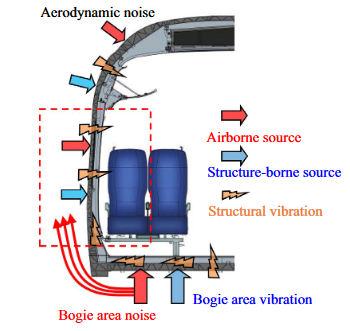
\includegraphics[width=0.6\textwidth]{fig/noise_transmission_path.png}
    \caption{Transmission path of exterior noise sources \cite{zhang_sound_2019}}
    \label{fig:my_label}
\end{figure}

\newpage
\section{Aims and objectives}

This thesis, in collaboration with Siemens Mobility Austria GmbH, aims to develop a finite-element model suitable for predicting the sound propagation from train underfloor area into the exterior environment around the carbody. 


The thesis is organised as follows. The fundamental background of the thesis is explained in Chap. \ref{chap:Theory}. Chap. \ref{chap:measurement} describes the outer pressure field measurement

\chapter{Fundamentals}
\label{chap:Theory}

\section{Governing equations and finite element formulation}

In this section, the governing equations for acoustics and the corresponding finite element formulation will be explained following Kaltenbacher \cite{kaltenbacher_numerical_2007, kaltenbacher_computational_2018}, Bergman \cite{bergman_computational_2018} and Heutschi \cite{heutschi_lecture_2016}.

\subsection*{Linear acoustic wave equation}
 Assuming an isentropic case, the basic equations of acoustics are based on the conservation of mass
\begin{equation}
	\frac{\partial \rho}{\partial t} + \nabla \cdot (\rho \boldsymbol{u}) = 0\text{,} \label{eq:conservation_of_mass}
\end{equation}
which is also called the continuity equation and the conservation of momentum
\begin{equation}
	\rho\frac{\partial \boldsymbol{u}}{\partial t} + \rho \boldsymbol{u}\cdot\nabla\boldsymbol{u} = -\nabla p + \nabla\cdot\left[\tau\right] + \boldsymbol{f}\text{.} \label{eq:conservation_of_momentum}
\end{equation}
Here, $\rho$ denotes the fluid density, $p$ the fluid pressure, $\boldsymbol{u}$ the particle velocity, $\left[\tau\right]$ the viscous stress tensor and $\boldsymbol{f}$ an external force density. If air is used as the medium for sound propagation, it can be considered as an inviscid fluid due to its low viscosity. Hence, $\nabla\cdot\left[\tau\right]$ in \cref{eq:conservation_of_momentum} can be neglected. Moreover, the external force density $\boldsymbol{f}$ will also be neglected for non-viscous fluids.

For linear acoustic wave propagation, the perturbation ansatz for the three acoustic quantities $\rho$, $p$ and $\boldsymbol{u}$ is used
\begin{equation}
	\rho = \rho_0 + \rho_a\text{;}\qquad p = p_0 + p_a\text{;}\qquad \boldsymbol{u} = \boldsymbol{u_0} + \boldsymbol{u_a}\text{,}
\end{equation}
whereby the quantities are split up in their mean $\square_0$ and alternating part $\square_a$. It is also assumed that the perturbations are small compared the mean parts
\begin{equation}
	\rho_a \ll \rho_0\text{;}\qquad p_a \ll p_0\text{;}\qquad \boldsymbol{u_a} \ll \boldsymbol{u_0}\text{.}
\end{equation}
Furthermore, it is assumed that the mean pressure $p_0$ and the mean density $\rho_0$ do not vary over space and time and a quiescent medium with no background flow ($\boldsymbol{u_0} = \boldsymbol{0}$) is considered. Applying the perturbation ansatz and all assumptions above to the conservation equations \cref{eq:conservation_of_mass}, \cref{eq:conservation_of_momentum} and neglecting all second order terms of the perturbations yields to
\begin{align}
	\frac{\partial \rho_a}{\partial t} + \rho_0\nabla\cdot\boldsymbol{u_a} &= 0\text{,} \label{eq:linearised_convervation_mass} \\ 
	\rho_0\frac{\partial \boldsymbol{u_a}}{\partial t} + \nabla p_a &= \boldsymbol{0}\text{,} \label{eq:linearised_convervation_momentum}
\end{align}
which are the linearized conservation equations of mass and momentum. Next, by applying a time derivative to \cref{eq:linearised_convervation_mass}, a space derivative to \cref{eq:linearised_convervation_momentum}, combining both equations and using the linearized pressure-density relation
\begin{equation}
	\rho_a = \frac{p_a}{c_0^2}\text{,}
\end{equation}
the linear acoustic wave equation for a homogeneous medium is obtained
\begin{equation}
	\frac{1}{c_0^2}\frac{\partial^2 p_a}{\partial t^2} - \nabla\cdot\nabla p_a = 0\text{,} \label{eq:wave_equation}
\end{equation}
where $c_0$ denotes the speed of sound in the propagation medium and depends on the material properties, namely the bulk modulus $K_0$ and the density $\rho_0$. Thereby, following relation holds \cite{fahy_foundations_2001, kinsler_fundamentals_2000}
\begin{equation}
	c_0 = \sqrt{\frac{K_0}{\rho_0}}\text{.}
\end{equation}

For a sinusoidal wave, which is for example excited by a harmonic source, the solution of \cref{eq:wave_equation} can be represented as
\begin{equation}
	p_a(\boldsymbol{x},t) = Re\lbrace\hat{p}_a(\boldsymbol{x})e^{j\omega t}\rbrace \text{,} \label{eq:sinusoidal_wave}
\end{equation}
with $\hat{p}_a$ being the pressure amplitude and $\omega$ being the angular frequency of oscillation. With the restriction to sinusoidal time dependency, the acoustic wave equation can be simplified to
\begin{equation}
	\nabla\cdot\nabla\hat{p}_a + \frac{\omega^2}{c_0^2}\hat{p}_a = 0 \text{,} \label{eq:helmholtz_equation}
\end{equation}
which is the famous Helmholtz equation. The pressure amplitude $\hat{p}_a$ depends only on the position in space.

\subsection*{Finite element formulation}

The linear acoustic wave equation \cref{eq:wave_equation} is also called the strong formulation of the linear acoustic PDE. To obtain the weak form or the variational formulation of the equation, it is multiplied by an appropriate test function $p'$ and integrated over the whole computational domain $\Omega$. Thus, the weak form of the PDE reads as
\begin{equation}
	\int_{\Omega}p'\frac{1}{c_0^2}\frac{\partial^2 p_a}{\partial t^2}\text{d}\Omega - \int_{\Omega}p'\nabla\cdot\nabla p_a\text{d}\Omega = 0\text{.} \label{eq:weak_form_PDE}
\end{equation}
Using the product rule for the divergence
\begin{equation}
	\nabla\cdot(f\boldsymbol{g}) = f\nabla\cdot\boldsymbol{g} + \nabla f \cdot \boldsymbol{g}\text{,}
\end{equation}
the second term in \cref{eq:weak_form_PDE} can be expressed as
\begin{equation}
	\int_{\Omega}p'\nabla\cdot\nabla p_a\text{d}\Omega = - \int_{\Omega}\nabla p'\cdot\nabla p_a\text{d}\Omega + \int_{\Omega}\nabla\cdot(p'\nabla p_a)\text{d}\Omega \text{.} \label{eq:noname_1}
\end{equation}
Applying the divergence theorem \cite{kreyszig_advanced, wiley_mathematics_1995}
\begin{equation}
	\int_{\Omega} \nabla\cdot \boldsymbol{g}\,\text{d}\Omega = \oint_{\partial \Omega} \boldsymbol{g}\cdot\boldsymbol{n}\,\text{d}\Gamma \text{,}
\end{equation}
to the last term of \cref{eq:noname_1} and inserting the obtained expression into \cref{eq:weak_form_PDE} leads to
\begin{equation}
	\int_{\Omega}p'\frac{1}{c_0^2}\frac{\partial^2 p_a}{\partial t^2}\,\text{d}\Omega + \int_{\Omega}p'\nabla\cdot\nabla p_a\,\text{d}\Omega - \oint_{\partial\Omega} p'\nabla p_a \cdot \boldsymbol{n}\,\text{d}\Gamma = 0\text{,} \label{eq:noname_2}
\end{equation}
where $\partial \Omega$ is the enclosed surface of $\Omega$ and $\boldsymbol{n}$ the surface normal vector.

In order to uniquely define the pressure $p_a$ in the domain $\Omega$, at least one boundary condition must be specified on the closed boundary surface $\partial \Omega$. A typical boundary condition in the acoustics is of Neumann type, which prescribes a normal traction
\begin{equation}
	\nabla p_a \cdot \boldsymbol{n} = p_n = -\rho_0\frac{\partial \boldsymbol{u_a}}{\partial t}\cdot\boldsymbol{n} = -\rho_0 a_n \label{eq:neumann_BC}
\end{equation}
at boundary $\Gamma_n$, where $a_n$ denotes the particle acceleration normal to $\Gamma_n$. The homogeneous Neumann boundary condition, i.e. $\nabla p_a \cdot \boldsymbol{n} = 0$, is also called sound hard boundary condition and can be used to model acoustic wall. For the inhomogeneous case ($p_n \neq 0$), it acts as an acoustic excitation on the boundary. Another boundary condition is of Dirichlet type, with prescribed pressure
\begin{equation}
	p_a = p_i \label{eq:dirichlet_BC}
\end{equation}
at boundary $\Gamma_i$. A homogeneous Dirichlet boundary condition ($p_i = 0$) is called sound soft boundary, which occurs mostly at a liquid-gas interface. Noticed that both sound hard and sound soft boundary conditions can lead to reflection of acoustic waves at the boundary.

Incorporating the Neumann boundary condition \cref{eq:neumann_BC} into \cref{eq:noname_2}, the final weak form is obtained, reading as
\begin{equation}
		\int_{\Omega}p'\frac{1}{c_0^2}\frac{\partial^2 p_a}{\partial t^2}\,\text{d}\Omega + \int_{\Omega}p'\nabla\cdot\nabla p_a\,\text{d}\Omega = \int_{\Gamma_n}p'p_n\,\text{d}\Gamma\text{,}
\end{equation}
which must be satisfied for all test functions $p'$ within the computational domain $\Omega$.

With the same procedure, the weak form of the Helmholtz equation \cref{eq:helmholtz_equation} can also be obtained
\begin{equation}
	\int_{\Omega}k^2\hat{p}_a\,\text{d}\Omega - \int_{\Omega}\nabla p' \cdot \nabla\hat{p}_a\,\text{d}\Omega + \oint_{\partial\Omega} p'\nabla \hat{p}_a \cdot \boldsymbol{n}\,\text{d}\Gamma = 0 \text{,}
\end{equation}
where $k$ is the wave number, being the angular frequency divided by the speed of sound. Again, Neumann boundary condition
\begin{equation}
	\nabla\hat{p}_a \cdot\boldsymbol{n} = \hat{p}_n
\end{equation}
at boundary $\Gamma_n$ or the Dirichlet boundary condition
\begin{equation}
	\hat{p}_a = \hat{p}_i
\end{equation}
at boundary $\Gamma_i$ can be incorporated.
\newpage

\section{Modeling of open domain problem}

To model exterior acoustics problems, in which the acoustic wave propagates in an open unbounded domain, special care needs to be taken.
A common practice is to truncate the propagation domain at a finite distance from the source and use homogeneous Neumann or Dirichlet boundary conditions, but this will result in an undesired reflection of the outgoing wave at the boundary \cite{nataf_absorbing_2013, kaltenbacher_numerical_2007}. One solution to such open-domain problem is to apply at the boundary a special condition, so-called absorbing boundary condition (ABC), which was first introduced by Engquist and Majda in 1977 \cite{Engquist_ABC_1977}. The other commonly used domain truncation technique is the perfectly matcher layer (PML), which is an additional acoustic domain surrounding the propagation domain, in which the acoustic waves are damped. The name "perfectly matched" refers to the matching impedances of both domains, and hence no reflections of the impinging wave occur at the domain boundary. Its concept was first introduced by Berenger in 1994 \cite{BERENGER_PML_1994} and was originally designed for the electromagnetic problem. There has been much research work on the PML-technique \cite{kaltenbacher_numerical_2007} and nowadays it is widely used in acoustic, electromagnetic or elastodynamic simulation \cite{nataf_absorbing_2013}. In the following, the basic concept of the PML technique is explained closely following Kaltenbacher \cite{kaltenbacher_numerical_2007, KALTENBACHER_PML_2013}.

We consider the linear wave equation \cref{eq:wave_equation} for one dimensional case with spatial coordinate $x$, which reads as 
\begin{equation}
	\frac{1}{c_0^2}\frac{\partial^2 p_a}{\partial t^2} -	\frac{\partial^2 p_a}{\partial x^2} = 0\text{.} \label{eq:1d_wave_equation}
\end{equation}

For plane wave propagation, the reflection coefficient $R$ at the interface between the propagation domain and the PML domain computes as
\begin{equation}
	R = \frac{Z_{\text{pml}} - Z_{\text{0}}}{Z_{\text{pml}} + Z_{\text{0}}}\text{,} \label{eq:reflection_coefficient_PML}
\end{equation}
with $Z_{\text{pml}} = \tilde{\rho}\tilde{c}$ the acoustic impedance in the PML region and $Z_{\text{0}} = \rho_0 c_0$ the specific acoustic impedance of the propagation medium, receptively. In order to make $R = 0$ to achieve zero reflection at the interface, $Z_{\text{pml}}$ has to match $Z_{\text{0}}$. Since the PML is an artificial domain, the two quantities $\tilde{\rho}$ and $\tilde{c}$ are free to be chosen in such a way that just their product equals $\rho_0 c_0$. By choosing complex values like
\begin{equation}
	\tilde{\rho} = \rho_0(1 - j\sigma_x)\text{;}\qquad \tilde{c} = \frac{c_0}{1- j\sigma_x}\text{,}
\end{equation}
the impedance matching $Z_{\text{pml}} = Z_{\text{0}}$ is still achieved. Here, $\sigma_x$ denotes a damping function in $x$-direction and it will be explained later in more detail. Furthermore, we consider the one dimensional Helmholtz equation, which is the time-harmonic case of \cref{eq:1d_wave_equation} and formulate for the PML region, we obtain
\begin{equation}
	\frac{\omega^2}{\tilde{c}^2}\hat{p}_a  +
	\frac{\partial^2 \hat{p}_a}{\partial x^2} = 0 \text{.} \label{eq:1d_helmholtz_equation}
\end{equation}
The first term in \cref{eq:1d_helmholtz_equation} can also be expressed by a complex wave number $\tilde{k}$
\begin{equation}
	\tilde{k} = \frac{\omega}{\tilde{c}} = \frac{\omega}{c_0}(1- j\sigma_x) = k(1-j\sigma_x)\text{.}
\end{equation}
The general solution for the pressure in the PML region then reads as
\begin{equation}
	p_a(x,t) = Re\lbrace\hat{p}_a e^{j(\omega t - \tilde{k}x)}\rbrace = Re\lbrace\hat{p}_a e^{j(\omega t - kx)} e^{-\sigma_x kx}\rbrace \text{.} \label{eq:noname_3}
\end{equation}
If $\sigma_x$ is chosen as constant, the pressure amplitude is decreased by the real term $e^{-\sigma_0 kx}$ with rising $x$, hence the acoustic wave is damped.

The formulation of PML so far works only for cases, where the impinging wave is normal to the interface between both regions. However, if the wave impinges to the normal vector of the interface at an angle $\phi$, then the acoustic impedances compute by
\begin{equation}
	Z_{\text{0}} = \frac{\rho_0 c_0}{\sin(\phi_1)}\qquad Z_{\text{pml}} = \frac{\tilde{\rho} \tilde{c}}{\sin(\phi_2)} \text{,}
\end{equation}
and the method will not be working. Therefore, we need to split up the linearized conservation equations \cref{eq:linearised_convervation_mass} and \cref{eq:linearised_convervation_momentum} into their spatial directions and introduce for each direction an artificial damping individually, which leads to the modified Helmholtz equation
\begin{equation}
	\eta_y\eta_z\frac{\partial}{\partial x}\left(\frac{1}{\eta_x}\frac{\partial\hat{p}_a}{\partial x}\right) + \eta_x\eta_z\frac{\partial}{\partial y}\left(\frac{1}{\eta_y}\frac{\partial\hat{p}_a}{\partial y}\right) + \eta_x\eta_y\frac{\partial}{\partial z}\left(\frac{1}{\eta_z}\frac{\partial\hat{p}_a}{\partial z}\right) + \eta_x\eta_y\eta_zk^2\hat{p}_a = 0 \text{,} \label{eq:modified_helmholtz_equation}
\end{equation}
where the functions
\begin{equation}
	\eta_i = 1 - j\frac{\sigma_i}{\omega}\text{,}\,i \in \lbrace x\text{,}y\text{,}z\rbrace
\end{equation}
were introduced, with $\sigma_i$ being the damping functions in the spatial direction $i\in\lbrace x\text{,}y\text{,}z\rbrace$. The full derivation of \cref{eq:modified_helmholtz_equation} can be found in \cite{kaltenbacher_numerical_2007}. A second method to derive \cref{eq:modified_helmholtz_equation} is the so-called complex coordinate stretching, which maps the solution of Helmholtz equation in the real coordinate space to a complex coordinate space. This is done by defining the mapping e.g. for $x$
\begin{equation}
	\tilde{x}(x) = x + \frac{1}{j\omega}\int_{0}^{x} \sigma_x(\tilde{x})\,\text{d}\tilde{x}\text{,}
\end{equation}
and thus, the derivative of the stretched coordinate $\tilde{x}$ with respect to its original $x$ is then
\begin{equation}
	\frac{\partial \tilde{x}}{\partial x} = 1 + \frac{\sigma_x}{j\omega} = \eta_x \text{.} \label{eq:derivative_stretched_coordinate}
\end{equation}
The derivative \cref{eq:derivative_stretched_coordinate} can be transformed as
\begin{equation}
	\frac{\partial}{\partial \tilde{x}} = \frac{1}{\eta_x}\frac{\partial}{\partial x}\text{.}
\end{equation}
In case of $\sigma_i = 0$, the stretched and the original coordinates are the same and $\eta_i = 1$ i.e. no mapping. Applying the coordinate stretching to all direction components, we obtain the operator
\begin{equation}
	\tilde{\nabla} = \left(\frac{1}{\eta_x}\frac{\partial}{\partial x}\text{,}\frac{1}{\eta_y}\frac{\partial}{\partial y}\text{,}\frac{1}{\eta_z}\frac{\partial}{\partial z} \right)^T \text{.} \label{eq:operator}
\end{equation}
Inserting the operator \cref{eq:operator} into the Helmholtz equation \cref{eq:helmholtz_equation} leads to the modified Helmholtz equation \cref{eq:modified_helmholtz_equation}.

In the following, the damping function $\sigma_i$ will be discussed in more detail. The performance of the PML is depending on the choice of the damping function. Different damping functions are shown in \cite{kaltenbacher_numerical_2007}. However, it can be proven that using a function that is zero at the interface between the propagation region and PML region and grows towards infinity with $\tilde{x}\rightarrow L$ works optimal for the Helmholtz equation \cite{kaltenbacher_numerical_2007,KALTENBACHER_PML_2013}. Such function is called inverse distance function and can be written as
\begin{equation}
	\sigma_x = \frac{c_0}{L - \tilde{x}}\text{.}
\end{equation}
Here, $c_0$ denotes the speed of sound in the propagation domain, $L$ denotes the thickness of the PML and the PML coordinate $\tilde{x}$ is zero at the domain interface and $L$ at the end of the layer. The speed of sound in the numerator is used for eliminating the dependency on $c_0$ in the damping term, which has the form $e^{-\sigma_x kx} = e^{-\sigma_x \frac{\omega}{c_0} x}$ (see \cref{eq:noname_3}). Another possibility besides using a constant damping function
\begin{equation}
	\sigma_x = \sigma_0c_0
\end{equation}
is to use a quadratic increase damping function like
\begin{equation}
	\sigma_x = \sigma_0c_0\frac{\tilde{x}^2}{L^2}\text{,}
\end{equation}
in this case, the constant damping factor $\sigma_0$ needs to chosen carefully for the given PML thickness $L$. Setting the damping factor too low could lead to insufficient damping of the acoustic wave in the PML domain, while setting it too high may cause numerical issues \cite{KALTENBACHER_PML_2013}. The tuning of the parameter is not necessary when using the inverse distance damping function, since it is dependent on the PML thickness $L$. A decreased thickness of the PML can be compensated by a higher value of the damping factor, but there is a limit where discretization errors become dominant \cite{KALTENBACHER_PML_2013}. Therefore, even for the optimal damping function, the thickness of the PML has to be chosen properly. Kaltenbacher \cite{KALTENBACHER_PML_2013} achieves good results with a PML thickness $t_\text{PML} = \frac{\lambda}{4}$ and $t_\text{PML} = \frac{\lambda}{8}$ in dependence of the acoustic wavelength $\lambda = \frac{c_0}{f}$ with a total error of $0.1\%$ in the propagation region. Furthermore, using a minimum of 2 linear elements or 1 quadratic element to resolve the PML region and choosing a similar element size for the propagation region and the PML region are suggested.

\newpage
\section{Fundamentals of noise measurement}

In this section, the most important terminologies in the noise and sound measurement technique will be briefly explained.

\subsection{Sound level}

The hearing of human does not respond linearly to the acoustic pressure, hence, a logarithmic scale is introduced when measuring the acoustic quantities \cite{fahy_foundations_2001}. The most commonly measured physical attribute of the sound is the sound pressure. Other important measures are sound particle velocity, sound intensity and sound power. The definitions of the logarithmic measures of the above mentioned quantities are presented below, following Kaltenbacher \cite{kaltenbacher_computational_2018} and Heutschi \cite{heutschi_lecture_2016}.


\subsubsection*{Sound pressure level}
The sound pressure level (SPL) is defined as
\begin{equation}
	L_p = 10\log_{10}\frac{p_{a\text{,rms}}^2}{p_\text{ref}^2} = 10\log_{10}\frac{p_{a\text{,rms}}}{p_\text{ref}}\,\text{dB}\text{,}
\end{equation}
where $p_\text{ref} = 2\cdot10^{-5}\,\text{Pa}$ denotes the reference sound pressure, which is often considered as threshold of human hearing at 1000 Hz \cite{sinambari_ingenieurakustik_2020}. $p_{a\text{,rms}}$ denotes the root-mean-square value of the acoustic pressure and is also called the effective pressure, which is defined as the square root of the average of the square of the pressure of the sound signal over a given time duration $T$ and reads as
\begin{equation}
	p_{a\text{,rms}} = \sqrt{\frac{1}{T} \int_{t_0}^{t_0 + T} p_a^2(t)\,\text{d}t}\text{.}
\end{equation}
It can be shown that for a sinusoidal acoustic wave like \cref{eq:sinusoidal_wave}, the effective pressure can be expressed as \cite{peterson_1972_handbook}
\begin{equation}
	p_{a\text{,rms}} = \frac{\hat{p}_a}{\sqrt{2}}\text{.}
\end{equation}

\subsubsection*{Sound velocity level}
Further, the sound velocity level (SVL) or the particle velocity level is defined as
\begin{equation}
	L_u = 10\log_{10}\frac{u_{a\text{,rms}}^2}{u_\text{ref}^2} = 10\log_{10}\frac{u_{a\text{,rms}}}{u_\text{ref}}\,\text{dB}\text{,} 
\end{equation}
with $u_\text{ref} = 5\cdot10^{-8}\,\frac{m}{s}$ the reference particle velocity in air and $u_{a\text{,rms}}$ the root-mean-square particle velocity. Again, the effective particle velocity can be expressed as
\begin{equation}
	u_{a\text{,rms}} = \frac{\hat{u}_a}{\sqrt{2}}
\end{equation}
for sinusoidal acoustic wave.

\subsubsection*{Sound intensity level}

The instantaneous acoustic intensity $\boldsymbol{I_a}$ is defined by the product of the acoustic pressure and the particle velocity
\begin{equation}
	\boldsymbol{I_a} = p_a \boldsymbol{u_a}\text{.}
\end{equation} 
For the sound intensity level (SIL), the averaged value of the instantaneous acoustic intensity is used, which computes by
\begin{equation}
	I_a^{\text{ave}} = |\boldsymbol{I_a^{\text{ave}}}| = \left|\frac{1}{T}\int_{t_0}^{t_0 + T} p_a \boldsymbol{u_a}\,\text{d}t\right|\text{.}
\end{equation}
The sound intensity level is then defined as
\begin{equation}
	L_I = 10\log_{10}\frac{I_a^{\text{ave}}}{I_\text{ref}}\,\text{dB}\text{,}
\end{equation}
with $I_\text{ref} = 10^{-12}\,\text{W/}\text{m}^2$ the reference sound intensity corresponding to the product of the reference sound pressure $p_\text{ref}$ and the reference particle velocity $u_\text{ref}$.

\subsubsection*{Sound power level}

The acoustic power is obtained by integrating the acoustic intensity over a closed surface and reads as
\begin{equation}
	W_a = \oint_{\Gamma} \boldsymbol{I_a}\cdot\,\text{d}\boldsymbol{s} = \oint_{\Gamma} \boldsymbol{I_a}\cdot\boldsymbol{n}\,\text{d}s \text{,}
\end{equation}
with $\boldsymbol{n}$ being the surface normal vector. The sound power level (SWL) is then defined as
\begin{equation}
	L_W = 10\log_{10}\frac{W_a^{\text{ave}}}{W_\text{ref}}\,\text{dB}\text{,}
\end{equation}
with $W_\text{ref} = 10^{-12}\,\text{W}$ being the reference sound power and $W_a^{\text{ave}}$ the averaged value of the acoustic power, which is computes for time harmonic case by
\begin{align}
	W_a^{\text{ave}} &= \int_{\Gamma}\left(\frac{1}{T} \int_{t_0}^{t_0 + T} Re\lbrace\hat{p}_a e^{j\omega t}\rbrace\,Re\lbrace\boldsymbol{\hat{u}_a} \cdot \boldsymbol{n} e^{j\omega t}\rbrace \, \text{d}t  \right)\,\text{d}s \\
	&= \frac{1}{2} \int_{\Gamma} Re\lbrace\hat{p}_a \boldsymbol{\hat{u}_a}^*\rbrace \cdot \boldsymbol{n}\,\text{d}s \text{,}
\end{align}
with $*$ denoting the conjugate complex.

\newpage
\subsection{Octaves and frequency bands}

A noise signal is often analyzed in the frequency domain in order to assess its frequency content. The frequency spectrum is divided into various frequency bands covering the hearing range of human, which varies from \SIrange{20}{20000}{\hertz}. The most commonly used frequency bands in the acoustic measurement are octave band and one-third octave band.

\subsubsection*{Octave band}
An octave band has a frequency span ratio of 2:1, which means that the upper limit frequency $f_u$ of the band is twice its lower limit frequency $f_l$, reads as
\begin{equation}
	f_u = 2f_l\,.
\end{equation}
The center frequency $f_m$ of the octave band is then calculated by their geometric mean
\begin{equation}
	f_m = \sqrt{f_l f_u} = \sqrt{2}f_l\,.
\end{equation}
The bandwidth $\Delta f$ of the octave band is given by
\begin{equation}
	\Delta f = f_u - f_l = \frac{f_u}{2} = \frac{f_m}{\sqrt{2}}\,.
\end{equation}
For acoustic measurements, the human audible range is split into 10 octave bands, with center frequencies being 31.5, 63, 125, 250, 500, 1000, 2000, 4000, 8000 and 16000 Hz.

\subsubsection*{Fractional octave bands}

If more detailed information about the frequency content of the noise is needed, fractional octave bands with higher frequency resolution can be used. In general, for a 1/n-octave band, the relation between the upper and the lower frequency limit is defined as
\begin{equation}
	f_u = 2^{^\frac{1}{n}}f_l\,.
\end{equation}
And the center frequency of 1/n-octave band is given by
\begin{equation}
	f_m = \sqrt{f_l f_u} = 2^{^{\frac{1}{2n}}}f_l\,.
\end{equation}
One can see that for $n = 1$, same expressions as for the octave band are obtained.

\begin{figure}[H]
	\centering
	\begin{subfigure}[b]{0.49\textwidth}
		\centering
		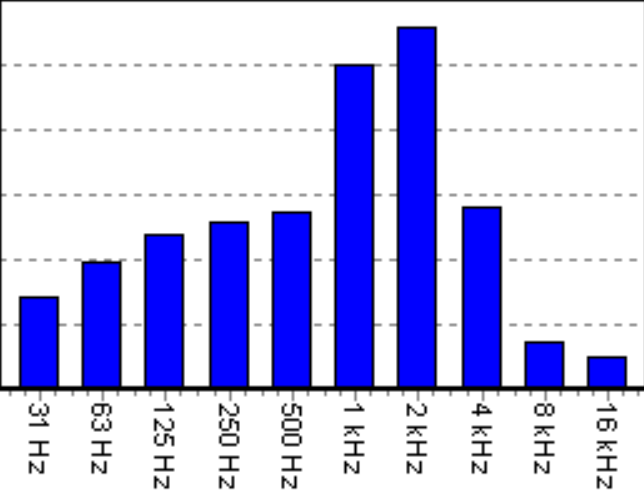
\includegraphics[width=0.8\linewidth]{fig/octave_band.PNG}
	\end{subfigure}
	\begin{subfigure}[b]{0.49\textwidth}
		\centering
		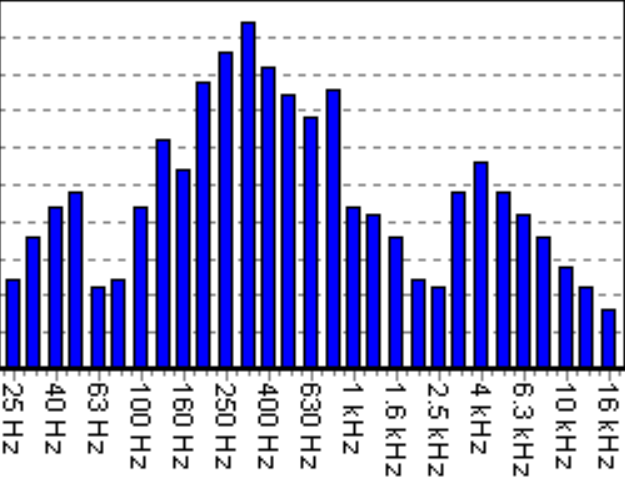
\includegraphics[width=0.8\linewidth]{fig/one_third_octave_band.PNG}
	\end{subfigure}
	\caption{Example octave band and 1/3-octave band spectra. Left: octave band spectrum. Right: 1/3-octave band spectrum. \cite{octave_band} }
	\label{fig:octave_band_filters}
\end{figure}

\noindent A widely used fractional octave band in the acoustic measurement is the 1/3-octave band, which is obtained by splitting each of the octave bands into three parts. Example sound spectra given in octave bands and 1/3-octave bands are shown in \cref{fig:octave_band_filters}. It can be seen that the spectrum in 1/3-octave bands contains more frequency bands than that of the octave band, allowing a more detailed analysis of the frequency content of the noise. Other common narrower fractional octave bands are for example 1/6-octave, 1/12-octave and 1/24-octave band.

\newpage
\subsection{Frequency weighting}

\begin{figure}[H]
	\centering
	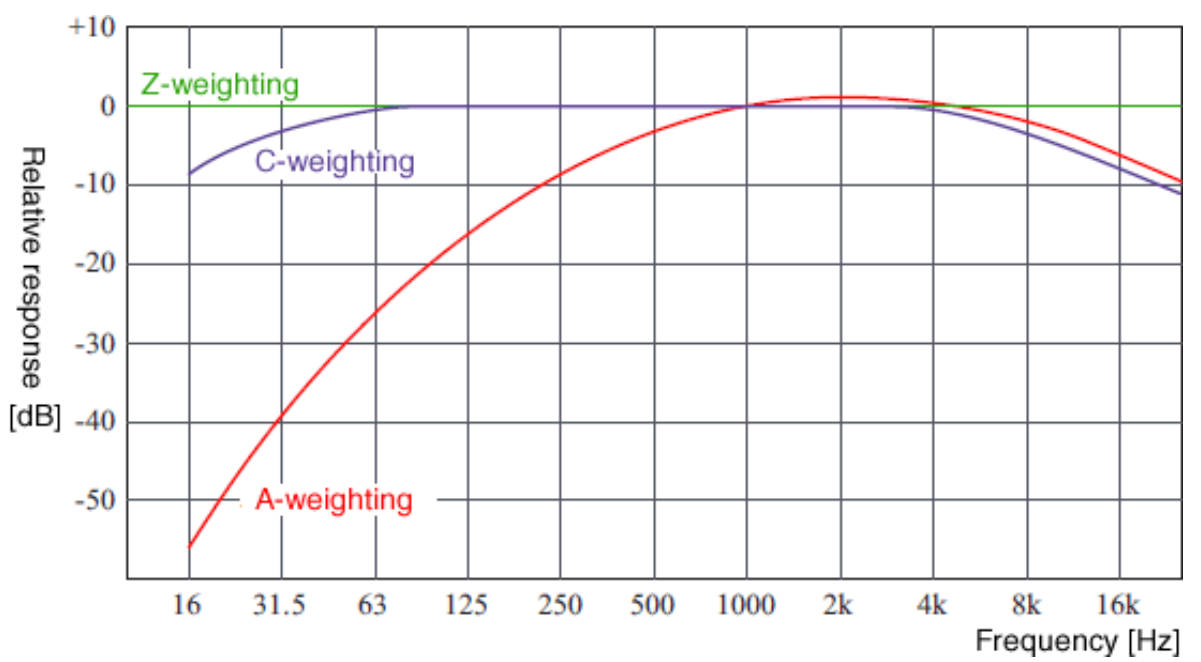
\includegraphics[width=0.8\textwidth]{fig/frequency_weighting.png}
	\caption{Frequency weighting (A, C and Z) \cite{Frquency_weighting}.}
	\label{fig:weighting}
\end{figure}

The human audible system does not respond equally to sound frequencies. It is more sensitive to frequencies between \SI{500}{\hertz} and \SI{8000}{\hertz} and less sensitive to lower-pitch and higher-pitch noises \cite{weighting_filters}. To match this frequency-dependent perception of sound loudness of the human ear, so-called frequency weighting filters have been defined, which can be seen as correction functions of the measured sound levels. However, the frequency response of the ear also depends on sound pressure level, at lower levels the effect is more pronounced than at higher levels \cite{heutschi_lecture_2016}. Therefore, several weighting filters have been defined. The most commonly used weighting functions are A-weighting and C-weighting, which are designed for low and high sound levels, respectively. If no weighting filter is applied to the measurement, it is also called Z-weighting. The response functions of the A, C and Z-weighting filters are shown in \cref{fig:weighting}.

In the ambient noise measurement, the most frequently used weighting is A-weighting. It can be calculated by the weighting function \cite{IEC61672}
\begin{equation}
	 R_A(f) = {12194^2 f^4 \over \left(f^2 + 20.6^2\right)\ \sqrt{\left(f^2 + 107.7^2\right)\left(f^2 + 737.9^2\right)}\ \left(f^2 + 12194^2\right)}\,,
\end{equation}
with $f$ being the frequency in \SI{}{\hertz}, the amplitude response of A-filter results in
\begin{equation}
	\text{A-weighting}(f) = 20\log_{10}\left(R_A(f)\right) - 20\log_{10}\left(R_A(1000)\right) \,. \label{eq:a_weighting}
\end{equation}
The second term in \cref{eq:a_weighting} is to ensure that the amplitude of the weighting function is normalized to \SI{0}{\decibel} at \SI{1000}{\hertz}, which can also be seen in \cref{fig:weighting}. Sound level measurements with A-weighting filter applied are expressed as dBA, or dB(A).

\newpage
\section{X-Wagen metro train}
\label{section:ubx_geometry}

In this thesis, the finite element modeling approach of underfloor noise prediction is applied on the X-Wagen metro from Siemens Mobility. A brief overview of the metro train is presented in the following section in order to provide a better insight into the modeled vehicle.

\begin{figure}[H]
	\centering
	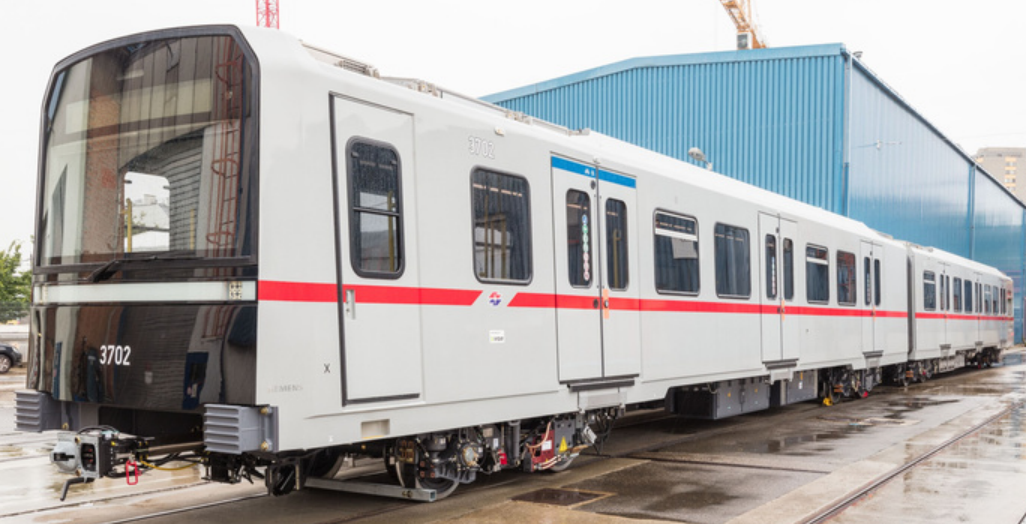
\includegraphics[width=0.8\textwidth]{fig/ubx_wiener_linien.PNG}
	\caption{The first X-Wagen metro train at Siemens Mobility plant Leberstraße \cite{foto_ubx}.}
	\label{fig:ubx_foto}
\end{figure}

The metro train Type X, also known as the X-Wagen, was developed by Siemens and is manufactured at the Siemens Mobility plant in Vienna. The third generation of the Vienna metro system aims to replace the old metro model Silverpfeil, which has been in operation since 1972. Siemens delivered the first X-Wagen (\cref{fig:ubx_foto}) in 2020, and the last vehicle is scheduled for delivery at the end of 2030.

\begin{figure}[H]
	\centering
	\begin{subfigure}[b]{\textwidth}
		\centering
		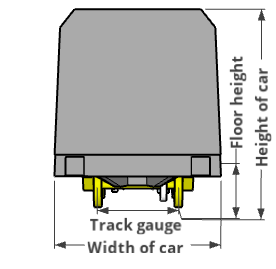
\includegraphics{fig/UBX_front_view_with_label_smaller.PNG}
		\caption{Front view}
	\end{subfigure}

	\begin{subfigure}[b]{\textwidth}
		\centering
		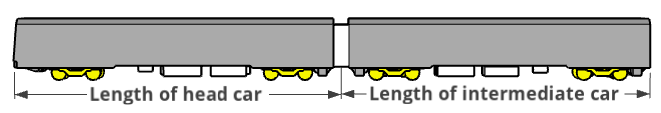
\includegraphics{fig/UBX_sketchup_model_side_view_with_label_2.PNG}
		\caption{Side view}
		\label{fig:ubx_model_sideview}
	\end{subfigure}
	
	\caption{3D model of the X-Wagen in its basic configuration.}
	\label{fig:ubx_sketup_model}
\end{figure}

The basic configuration of the train, as shown in \cref{fig:ubx_foto} and \cref{fig:ubx_model_sideview}, consists of two metro cars, a non-motorized head car where the driver's cab is located, and a motorized intermediate car. One section of the metro car is about \SI{2.85}{\meter} in width and \SI{3.6}{\meter} in height and has a length of \SI{19.1}{\meter} for the head car and \SI{18.3}{\meter} for the intermediate car, respectively. The train has a standard track gauge of \SI{1.425}{\meter}, and the car floor is about \SI{0.95}{\meter} over top of the rail. In the operating configuration, the metro train is made up of 6 sections consisting of 2 head cars and 4 intermediate cars with a length of over \SI{110}{\meter}.

\begin{figure}[H]
	\centering
	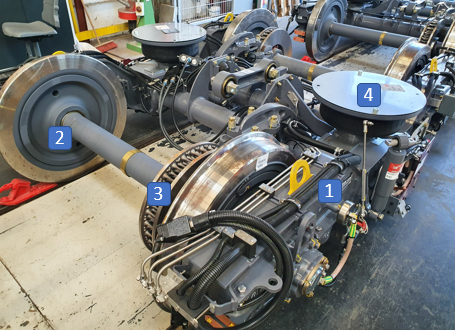
\includegraphics{fig/running_bogie_with_labels.PNG}
	\caption{A non-driven bogie from the head car. Main components are numbered as follows; (1) bogie frame, (2) wheel and axle, (3) brake disc, (4) air suspension.}
	\label{fig:bogie_foto}
\end{figure}

The main components in the train underfloor are the bogies and other supporting units like air compressors, electrical transformers, etc.
Each metro car is equipped with two bogies. While the bogies at the front car are non-driven, the intermediate car bogies are driven by traction motors. A non-driven bogie from the front car is shown in \cref{fig:bogie_foto} with the main components numbered. These are the bogie frame with length of about \SI{3}{\meter}, the wheels with \SI{0.85}{\meter} diameter and a distance of \SI{2}{\meter} to each other, the axles, and the air suspensions. Each axle is equipped with one brake disk and one brake caliper unit, and the brake components of both axles are arranged in an anti-symmetric order.

\begin{figure}[H]
	\centering
	\begin{subfigure}[b]{0.48\textwidth}
		\centering
		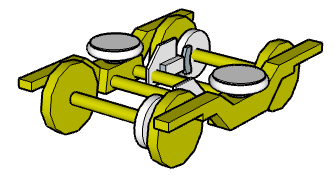
\includegraphics{fig/running_bogie_sketchup.PNG}
		\caption{Perspective view}
	\end{subfigure}
	\begin{subfigure}[b]{0.48\textwidth}
		\centering
		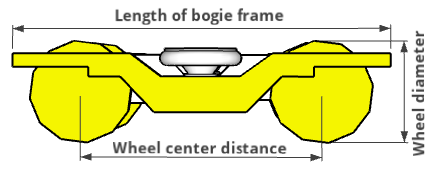
\includegraphics[width=\linewidth]{fig/running_bogie_sideview_with_labels.PNG}
		\caption{Side view}
		\label{fig:bogie_side_view}
	\end{subfigure}
	\label{fig:bogie_3d_model}
	\caption{Simplified 3D model of the non-driven bogie containing the main components as described in \cref{fig:bogie_foto}.}
\end{figure}

A simplified 3D model of the non-driven bogie containing the mentioned main components is shown in \cref{fig:bogie_3d_model}. One can see that the brake components introduce asymmetry into the bogie geometry. If they are disregarded, the symmetry of the bogie can be exploited, and the full model can be represented by a one-fourth model, which is used in the latter finite element modeling in \cref{chap:FEM}.

Finally, the mentioned dimensions of the metro car and of the bogie components in this section are summarized in \cref{tab:vehicle_dimensions}.
\begin{table}[H]
	\caption{Dimensions of metro car and bogie as shown in \cref{fig:ubx_sketup_model} and \cref{fig:bogie_side_view}.}
	\centering
	\begin{tabular}{lc}
		\toprule
		Parameter                    	   &  Dimension (mm)    \\
		\midrule
		\textbf{Metro car} 				   & 		 \\
		Width of car                       & 2,850   \\
		Height of car  					   & 3,588   \\
		Length of head car  			   & 19,125  \\
		Length of intermediate car 		   & 18,250  \\
		Floor height above top of rail     & 948     \\
		Track gauge              		   & 1,435   \\
		\textbf{Bogie} 					   & 		 \\
		Length of bogie frame    		   & 3,076   \\
		Wheel center distance 			   & 2,000   \\ 
		Wheel diameter  				   & 850     \\ 
		\bottomrule
	\end{tabular}
	\label{tab:vehicle_dimensions}
\end{table}

\chapter{Measurements}
\label{chap:measurement}

In order to be able to validate the results obtained from the finite element simulation (see \cref{chap:results}), specific measurements have been carried out.
In this chapter, the acoustic power measurement of the sound source and the outer pressure field measurement around the car body are presented.
The resulting sound power spectrum of the omnidirectional loudspeaker provides simulation input for the finite element analysis in section \ref{section:boundary_conditions}.
Furthermore, the measurement results of outer pressure field serve as validation for the finite element model in \cref{chap:results}.

\section{Characterization of sound source}
\label{section:SWL_measurement}

Two important characteristics of a sound source are directivity and sound power. For the validation measurement, a dodecahedron loudspeaker, type Brüel \& Kjaer 4292-L, is used as excitation, which can be treated as an omnidirectional sound source.
Hence, only the sound power emitted by the loudspeaker is interesting.
In the following, the acoustic power spectrum of the sound source is measured following ISO 9614-2 \cite{din19969614}.

\subsection*{Measurement setup}

In \cref{fig:soundpowersetup} the measurement setup for the determination of sound power levels is shown.
The omnidirectional loudspeaker was placed on a reflective concrete floor and was enveloped by a 1m x 1m x 1m reference box.
The loudspeaker was driven by a reference amplifier with pink noise as an input signal (\cref{fig:signalgenerator}).
In order to reduce fluctuations in output power, the amplifier was switched on and warmed up for at least 20 minutes before the start of the measurement.
% weniger Absätze verbessern den Lesefluss.
% Ein Absattz sollte zumindest 3 Sätze haben
The measurement was carried out according to the ISO 9614-2 standard, in which the sound power is determined from intensity measurement over measurement surfaces.
This method has the advantage that room reflections and any sound sources outside of the reference box do not influence the measurement result.
The intensity measurements were done using the Brüel \& Kjaer sound intensity probe kit type 3654, which includes a pair of microphones that are placed face to face with each other, separated by a spacer.

% Absatz "2 microphone Intensity measurement"
This method of intensity measurement is also called two-microphone method or $p-p$ method.
% jeder Satz in einer eigenen Zeile gibt besser git-diffs ...
Instead of direct measurement, the particle velocity is obtained by a finite-difference approximation to the pressure gradient \cite{jocobsen_2005, moschioni_2008}.
% willst du den ganzen Ansatz zitieren? Dann ist [ref] nach . richtig.
% Ansonsten wäre dies ein Anbsatz mit "2 microphone Intensity measurement" als Thema
In the following, the basic concept of sound power measurement using the two-microphone method is shown. The relation between particle velocity $\boldsymbol{u_a}$ and the acoustic pressure $p_a$ is described by the Euler equation of motion,
\begin{equation}
    \rho_0 \frac{\partial \boldsymbol{u_a}}{\partial t} = -\nabla p_a \text{.} \label{eq:euler_equatioin}
\end{equation}
In the intensity measurement using the two-microphone method (\cref{fig:scanningmethod}), the intensity probe is moved over the measurement surface with a constant speed and is kept perpendicular to the scanned area so that only the normal component of the particle velocity is captured. Furthermore, the normal component of the pressure gradient in \cref{eq:euler_equatioin} is approximated by the finite difference of the measured pressures. \Cref{eq:euler_equatioin} for the normal component then reads as
\begin{equation}
	\rho_0\frac{\partial(\boldsymbol{u_a} \cdot \boldsymbol{n})}{\partial t} = -\nabla p_a \cdot \boldsymbol{n} \approx -\frac{p_2 - p_1}{\Delta r}\text{,}
\end{equation}
with $p_1$ and $p_2$ being the measured pressure of the microphone closer and further from the incident sound wave, respectively, $\Delta r$ being the thickness of the spacer, and $\boldsymbol{n}$ the unit normal vector of the measurement surface. Hence, the normal particle velocity $u_n$ can be expressed as
\begin{equation}
   u_n = \boldsymbol{u_a} \cdot \boldsymbol{n} = \int\frac{(p_1 - p_2)}{\rho_0 \Delta r}\dif t \text{.}
\end{equation}
The normal component of the sound intensity is then obtained by the product of the approximated particle velocity and the mean of the measured pressures
\begin{equation}
    I_n = \boldsymbol{I_a} \cdot \boldsymbol{n} = p_a u_n = \frac{p_1 + p_2}{2} \int\frac{(p_1 - p_2)}{\rho_0 \Delta r}\dif t\text{.}
\end{equation}
Each partial measurement surface is scanned twice, using a vertical and a horizontal scan path, respectively. The obtained result is the spatially averaged intensity $\langle I_{n}\rangle$. The sound power of a single measurement surface is then given by the product of the spatial average intensity and the surface area by
\begin{equation}
    W_i = \langle I_{n\text{,}i}\rangle S_i\,.
\end{equation}
The total sound power of the enclosed sound source is then given by the sum of the sound power of each measurement surface and reads as
\begin{equation}
    W_{total} = \sum_{i = 1}^{N} W_i\,.
\end{equation}

% Beispiel für eine Grafik
\begin{figure}[H]
\begin{center}
\includegraphics[width=0.8\textwidth]{fig/Sound_power_measurement.png}
\caption{Setup for sound power measurement.}
\label{fig:soundpowersetup}
\end{center}
\end{figure}

\begin{figure}[H]
     \centering
     \begin{subfigure}[b]{0.5\textwidth}
         \centering
         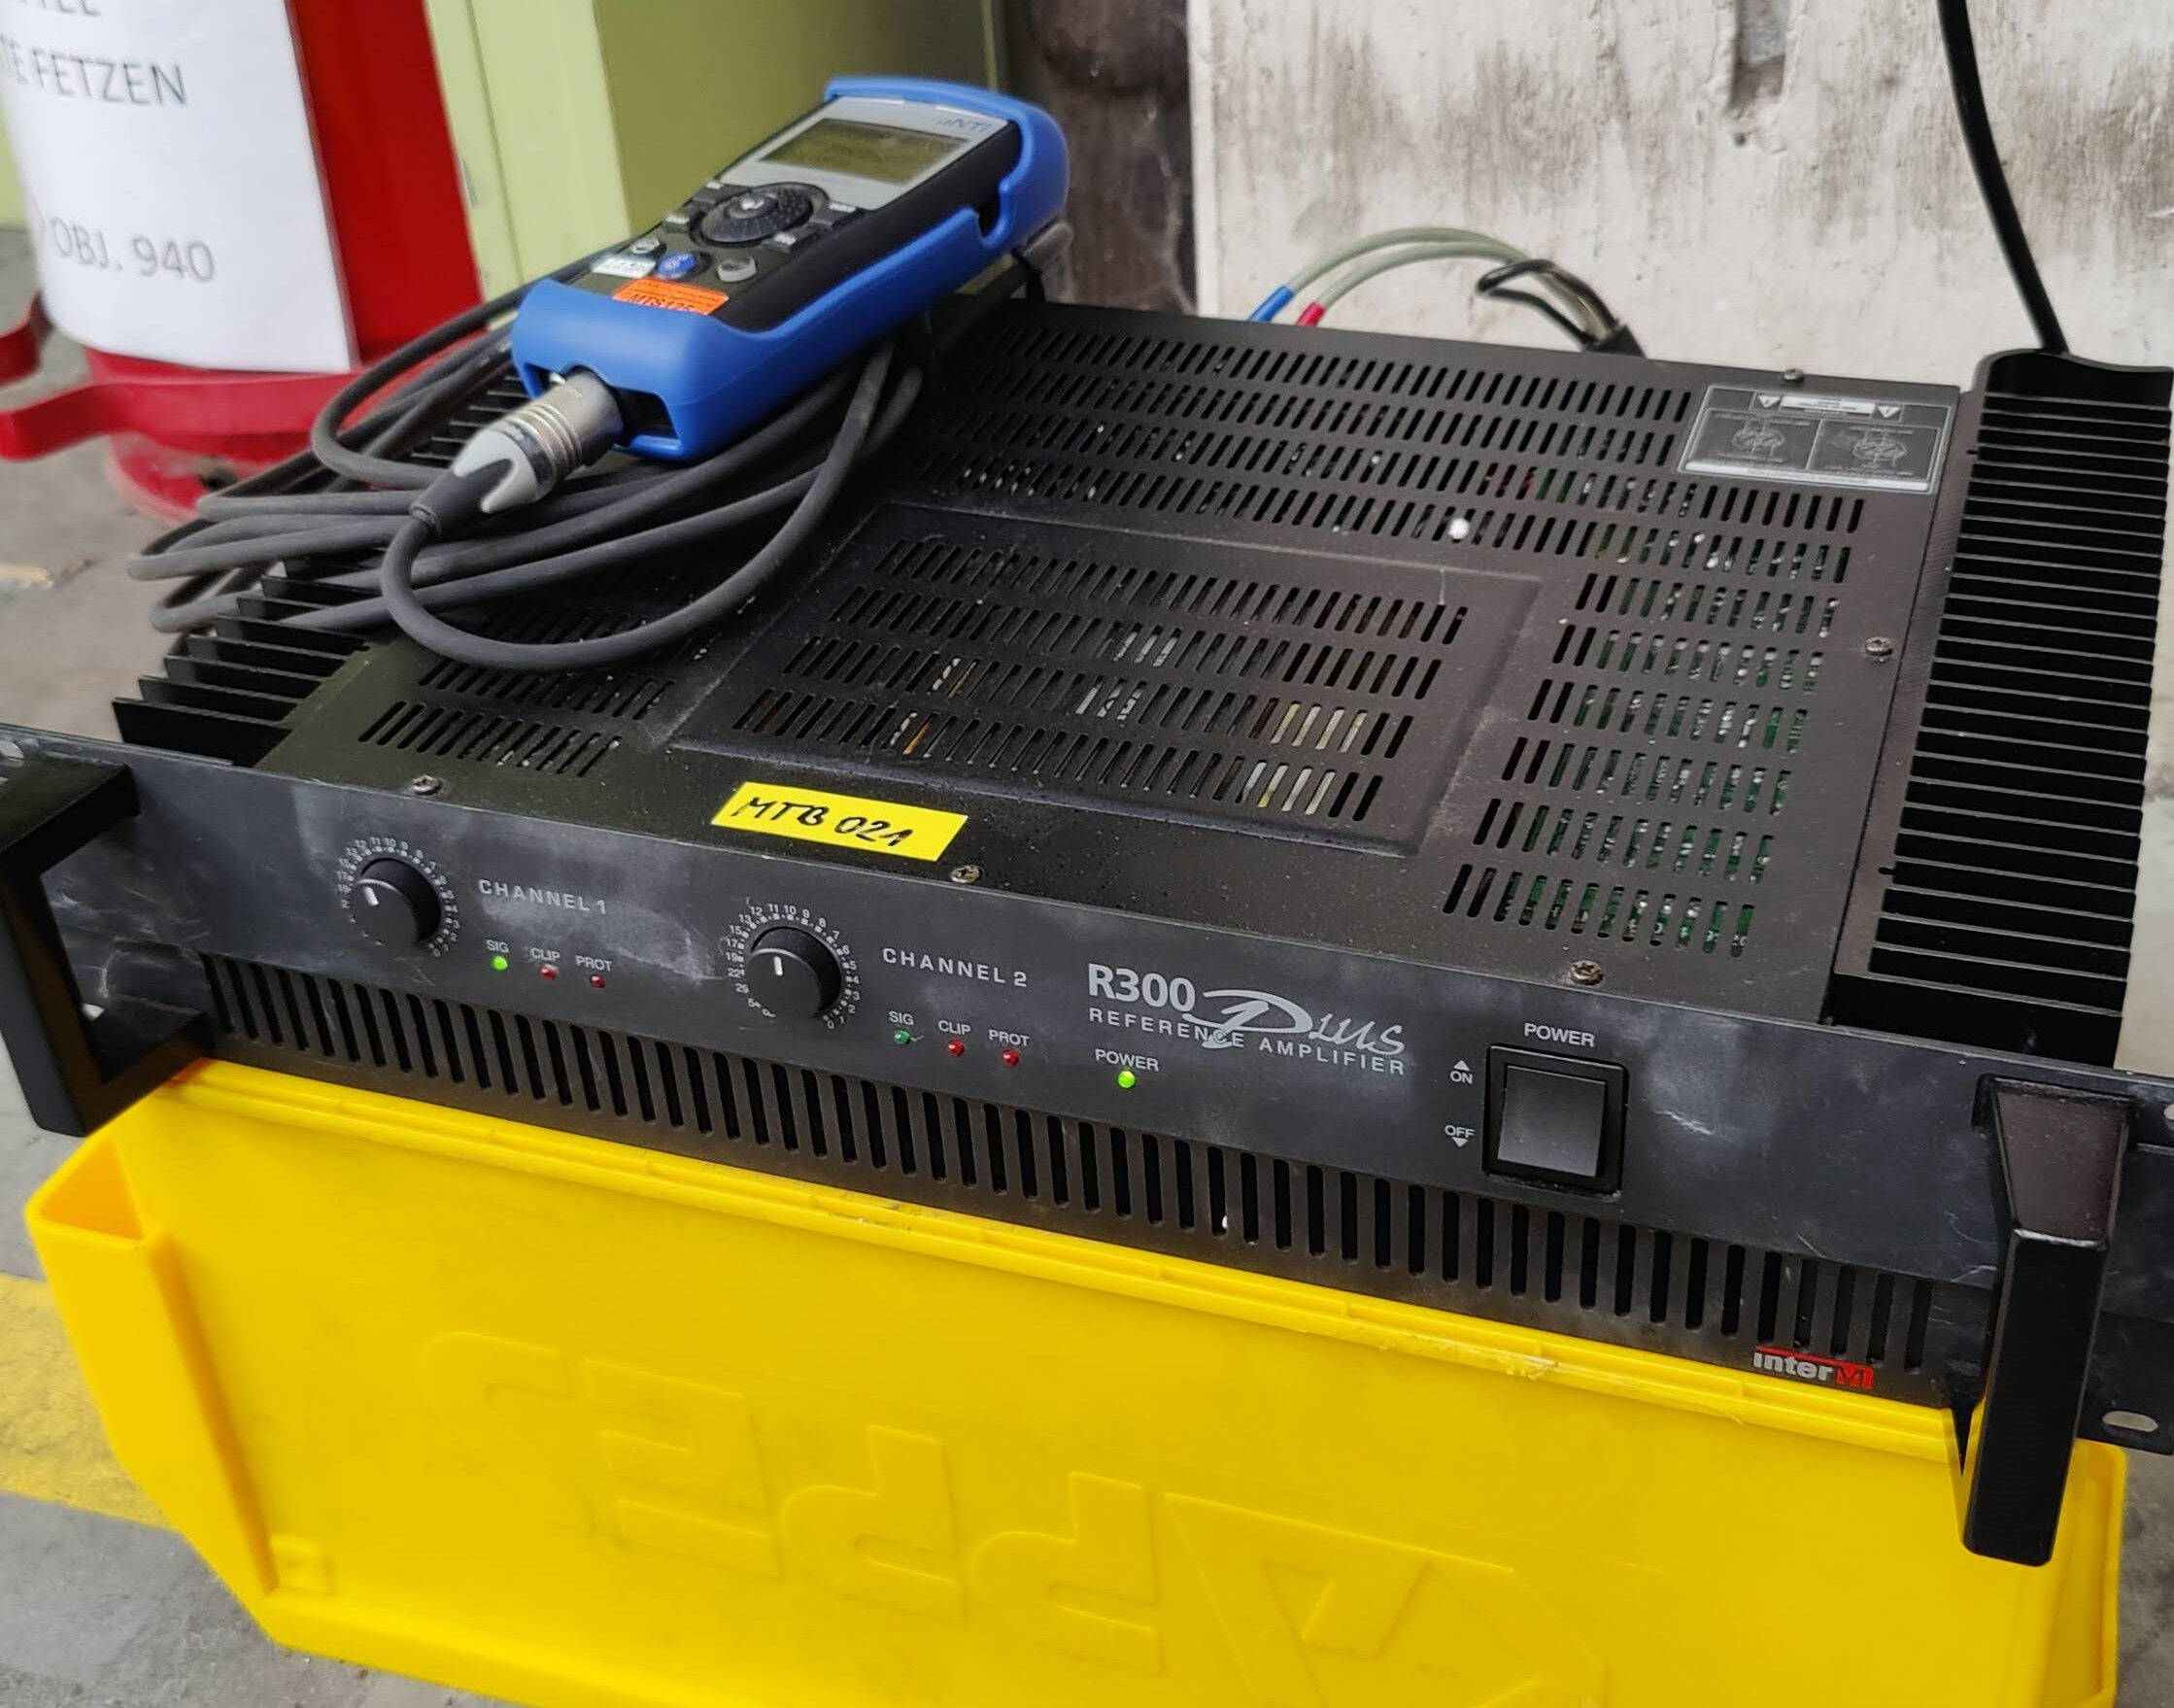
\includegraphics[width=\textwidth]{fig/amplifier_and_signal_generator.jpg}
         \caption{Inter-M R300 Plus reference amplifier}
     \end{subfigure}
     \hspace{0.1\textwidth}
     %\hfill
     \begin{subfigure}[b]{0.3\textwidth}
         \centering
         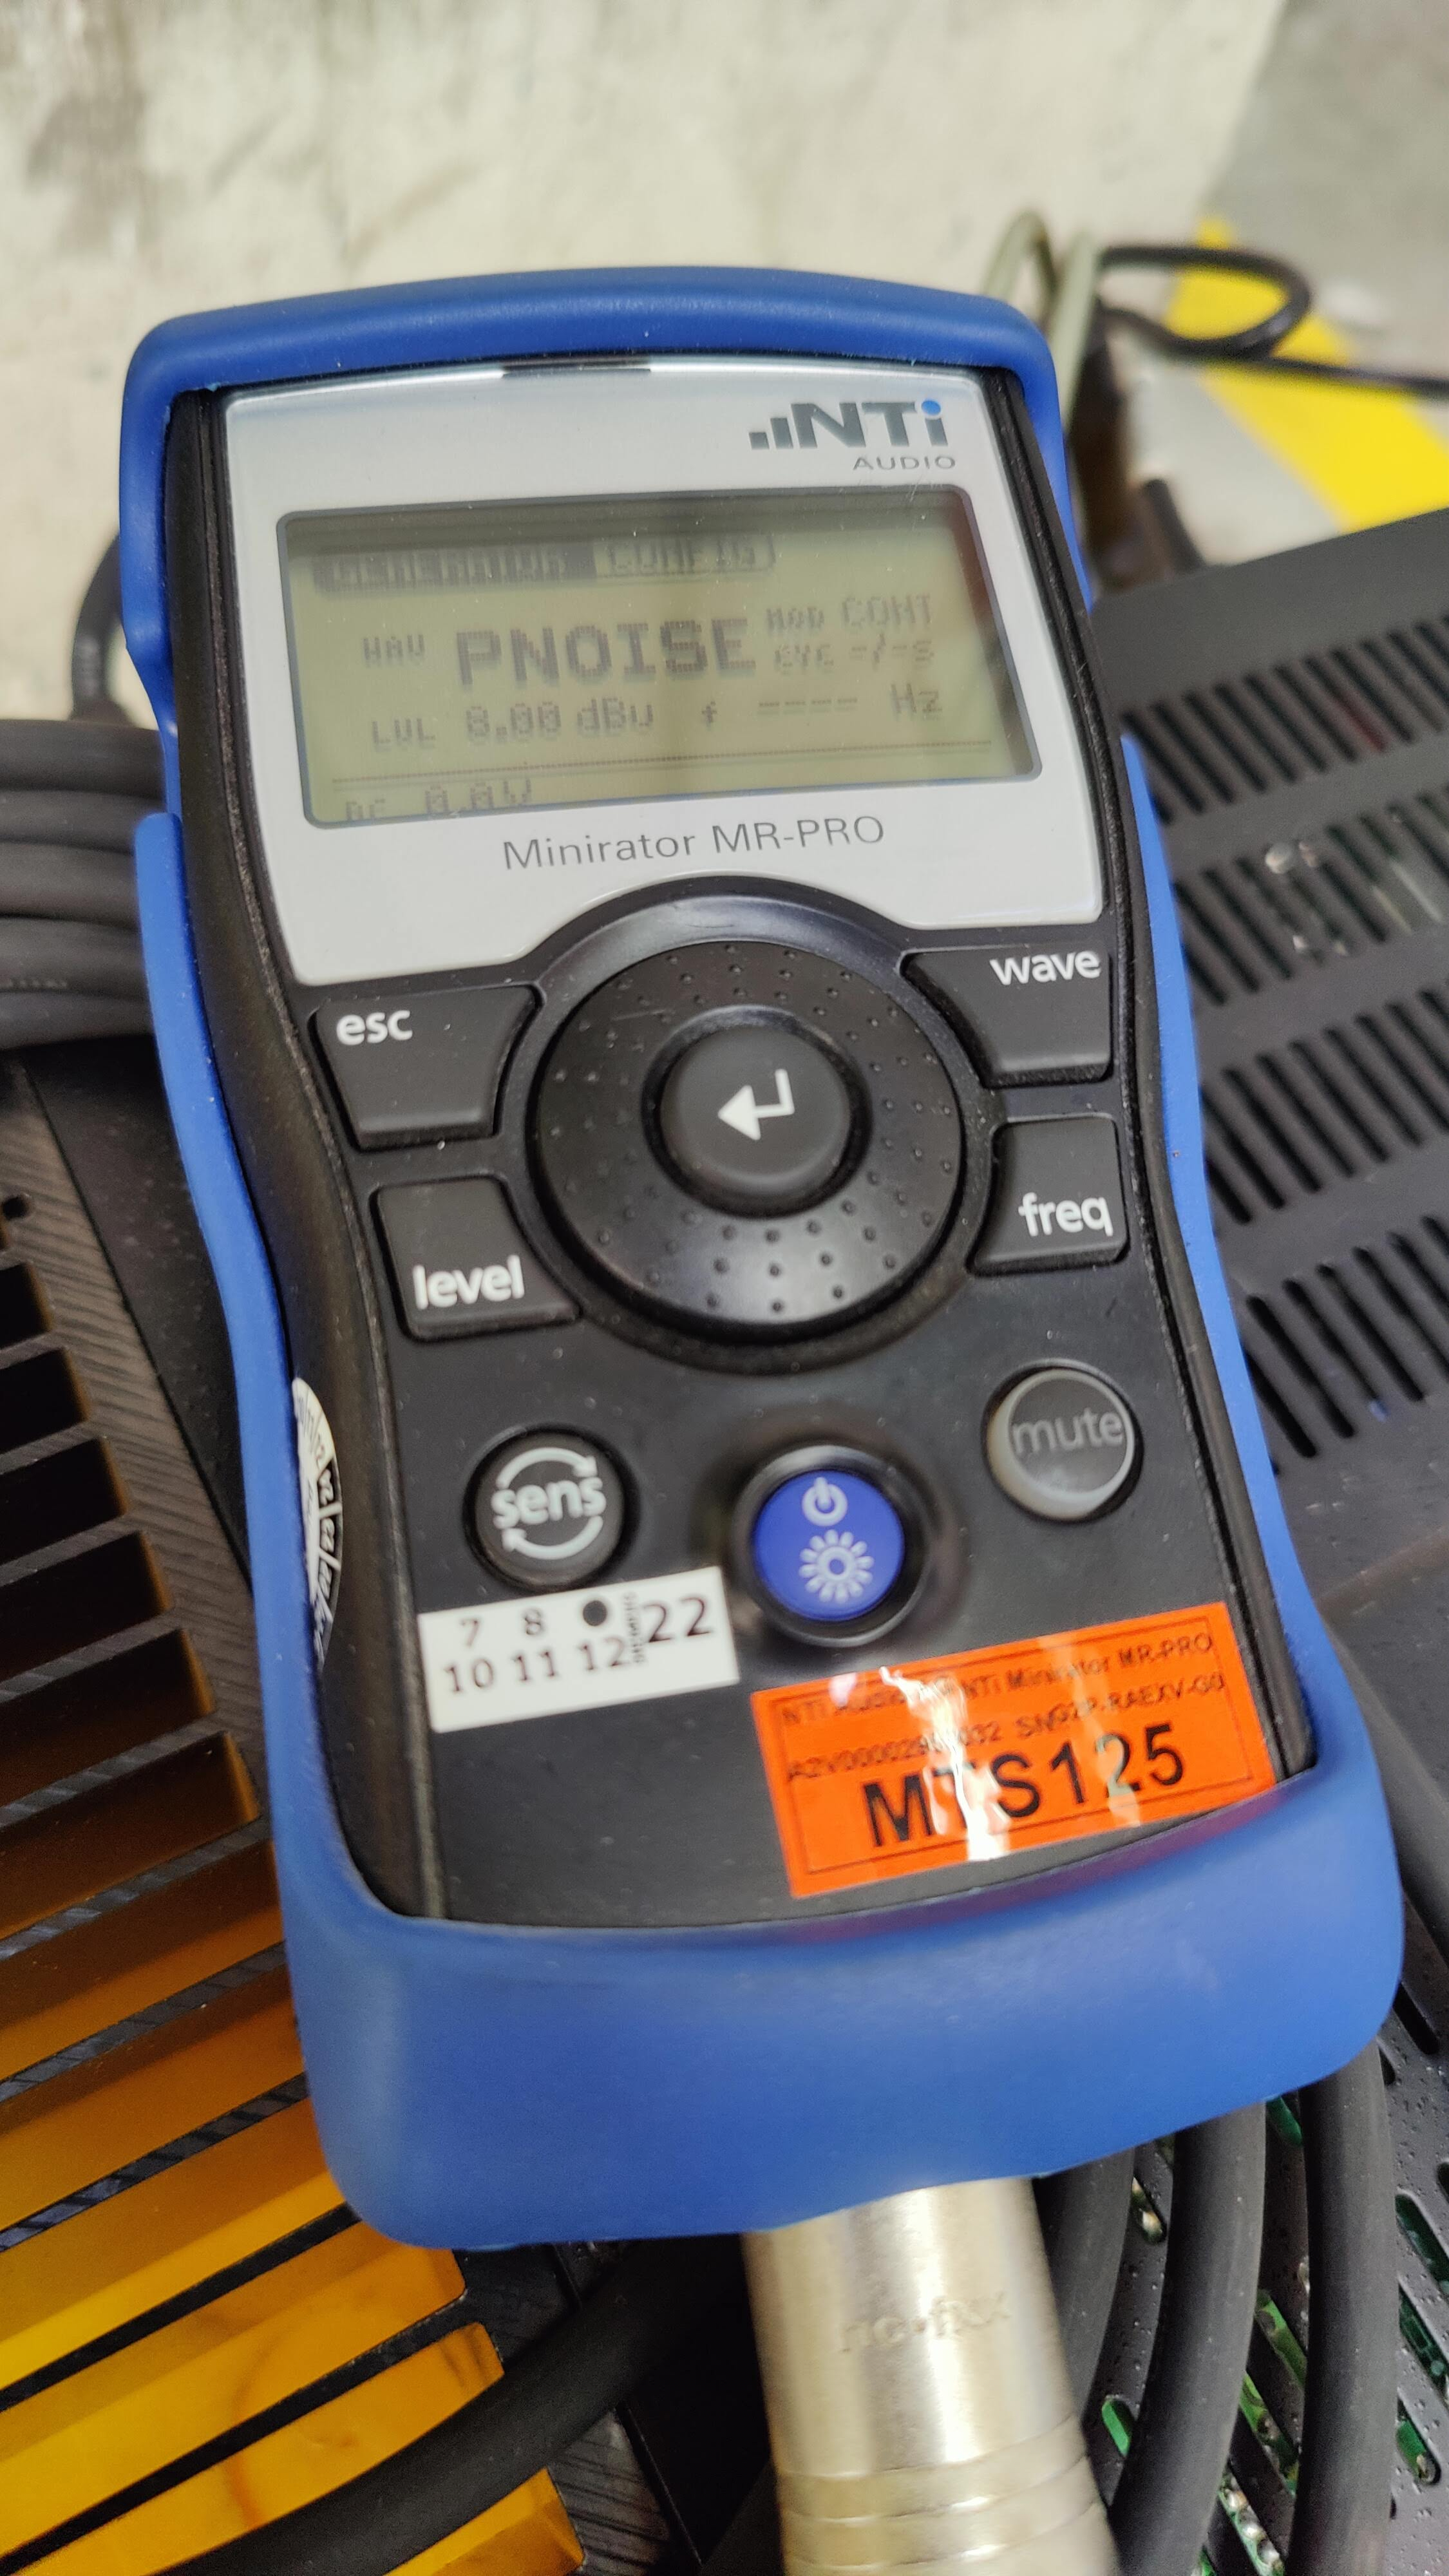
\includegraphics[width=\textwidth]{fig/signal_generator.jpg}
         \caption{NTI Minirator MR-PRO}
     \end{subfigure}
        \caption{Signal generator and amplifier.}
        \label{fig:signalgenerator}
\end{figure}

\begin{figure}[H]
\begin{center}
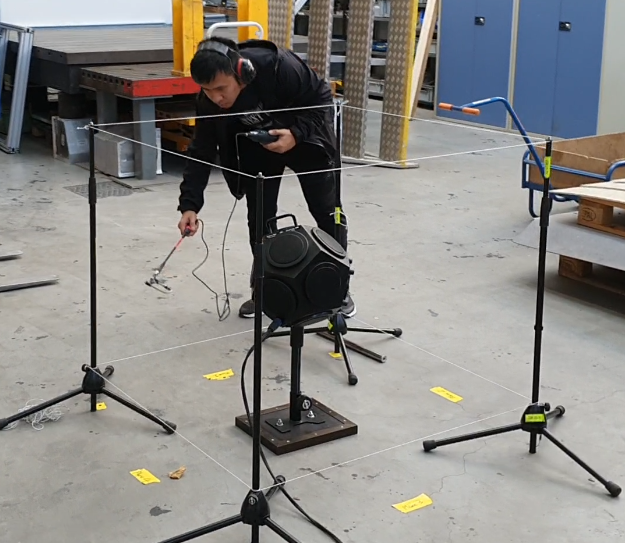
\includegraphics[width=12cm]{fig/Sound_power_measurement_2.png}
\caption{Intensity measurement using the two-microphone method according to ISO 9614-2 \cite{din19969614}.}
\label{fig:scanningmethod}
\end{center}
\end{figure}

\subsection*{Measurement results}

The measurement is post-processed using the Brüel \& Kjaer type 2270 hand-held analyzer and the result is shown in one-third octave band spectra. \Cref{fig:SWL} shows the measured non-weighted (Z-weighting) sound power level (SWL ref \SI{1}{\pico\watt}) from \SIrange{100}{2000}{\hertz}. The measurement was carried out twice, and the deviation of both measurements was within \SI{0.3}{\dB} in total power. For the finite element simulation, the averaged value of both measurements as shown in \cref{fig:average_SWL} was used.

\begin{figure}[H]
     \centering
     \begin{subfigure}[b]{0.9\textwidth}
         \centering
         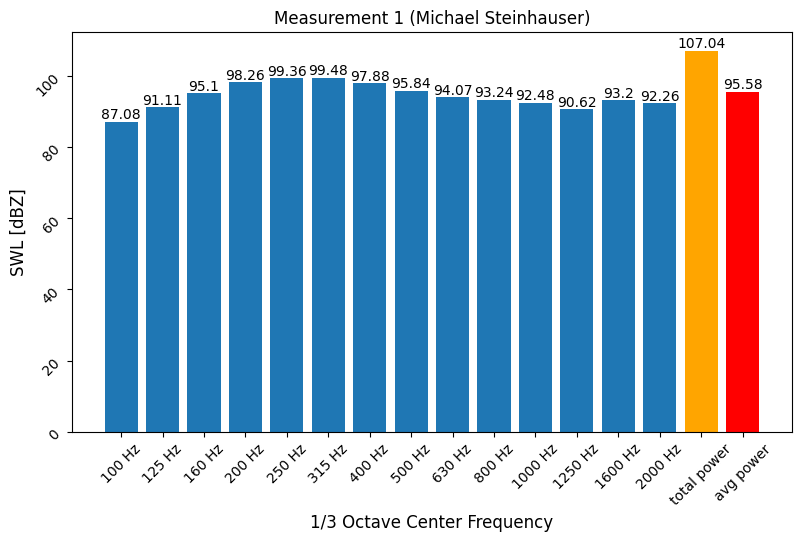
\includegraphics[width=\linewidth]{fig/SWL_1.png}
         \caption{Measurement series 1}
     \end{subfigure}
     \par\bigskip
     %\hspace{0.1\textwidth}
     %\hfill
     \begin{subfigure}[b]{0.9\textwidth}
         \centering
         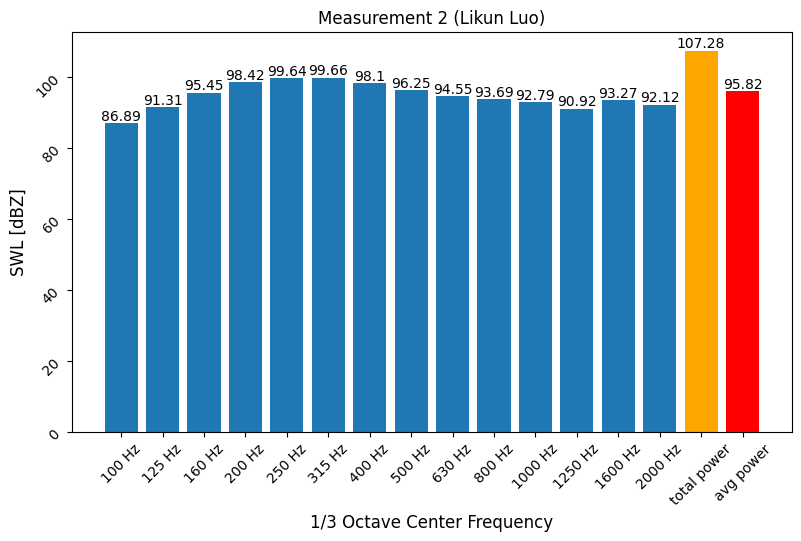
\includegraphics[width=\linewidth]{fig/SWL_2.png}
         \caption{Measurement series 2}
     \end{subfigure}
\end{figure}

\begin{figure}[H]\ContinuedFloat
     \centering
     \begin{subfigure}[b]{0.9\textwidth}
         \centering
         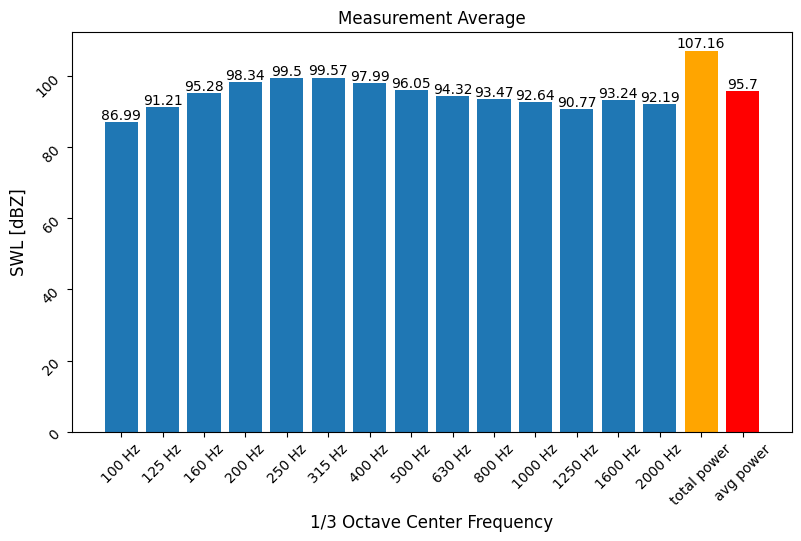
\includegraphics[width=\linewidth]{fig/SWL_average.png}
         \caption{Averaged value of both measurement series}
         \label{fig:average_SWL}
     \end{subfigure}
     
        \caption{Sound power spectra in 1/3-octave bands, SWL in \SI{}{\dB} ref \SI{1}{\pico\watt}.}
        \label{fig:SWL}
\end{figure}


\section{Pressure field measurement on a standing metro train}
\label{sec:pressure_field_measurement}

In this section, we describe the sound pressure measurements, which were done on a standing UBX metro with controlled excitation.
The reason to perform measurements under standstill conditions was to avoid the uncertainties introduced by the complex real sources (e.g., wheel-rail interaction) in dynamic conditions. With this approach, the quality of the finite element model can be better assessed.

\subsection*{Measurement setup}

The measurement was performed on October 4, 2022, at the company premises of Siemens Mobility Austria in 1110 Vienna. The measurement setup is shown in \cref{fig:outersetup}. \Cref{fig:ubxfrontview} shows the front car of the measurement vehicle of type Siemens U-Bahn Wien X. In order to approximate free field conditions as closely as possible, the measurement vehicle was parked in a relatively empty area of the company premises to avoid environmental reflections as much as possible.

To evaluate the outer pressure field close to the car body, 10 pressure microphones were arranged in a line array order, allowing simultaneous measurement along the height direction. As shown in \cref{fig:ubxsideview}, the microphones were attached on a tripod at a distance of half a meter to each other, the position of the microphones started at 0.5 m and ended at 5 m above ground.

The acoustic excitation came from an omnidirectional loudspeaker with pink noise as an input signal, using identical settings as in the previous acoustic power measurement. The loudspeaker was placed beneath the car underframe in the empty space between the bogie axle and the wheel axle, at about 55 cm above the ground (see \cref{fig:loudspeakerposition}). Measurements were performed with two different loudspeaker locations: one at the front of the bogie (Position A) and the other at the rear (Position B), as marked in \cref{fig:ubxsideview}. The aim was to evaluate the possible asymmetric effect caused by the anti-symmetric layout of the bogie components (e.g., brake discs); also, it provides validation for the finite element model, which will exploit the symmetry using the image-source technique.

Due to the limited availability of the measurement vehicle, the measurement was concentrated on only one side of the vehicle near the front bogie. In \cref{fig:microphoneposition}, all measurement positions of the microphone array are shown and labeled. Position a is the starting position of measurement, it lies on the centerline of the bogie frame, 10 cm away from the carbody edge (see \cref{fig:position_a}). The full description of measurement positions is found in \cref{tab:measurement_positons}.

\begin{table}[H]
	\begin{tabular}{cc}
		\toprule
		Position  & Description                                                                     \\
		\midrule
		a              & on bogie centerline, 10 cm away from carbody edge                              \\
		b              & 50 cm out of bogie centerline in front direction, 10 cm away from carbody edge  \\
		c              & 100 cm out of bogie centerline in front direction, 10 cm away from carbody edge \\
		d              & 50 cm out of bogie centerline in rear direction, 10 cm away from carbody edge   \\
		e              & 100 cm out of bogie centerline in rear direction, 10 cm away from carbody edge  \\
		f              & on bogie centerline, 50 cm away from carbody edge                              \\
		g              & on bogie centerline, 100 cm away from carbody edge                             \\
		h              & on bogie centerline, 150 cm away from carbody edge                             \\ 
		i              & on bogie centerline, 200 cm away from carbody edge                             \\ 
		\bottomrule
	\end{tabular}
	\caption{Description of measurement positions.}
	\label{tab:measurement_positons}
\end{table}
\noindent At each measurement position, the multi-channel time-varying signal of the pressure field was captured by the Müller-BBM PAK MKII data acquisition system. The duration of a single measurement run was set to 15 seconds. The captured time signal will be post-processed using the provided Müller-BBM PAK software suite.

\begin{figure}[H]
     \centering
     \begin{subfigure}[b]{0.7\textwidth}
         \centering
         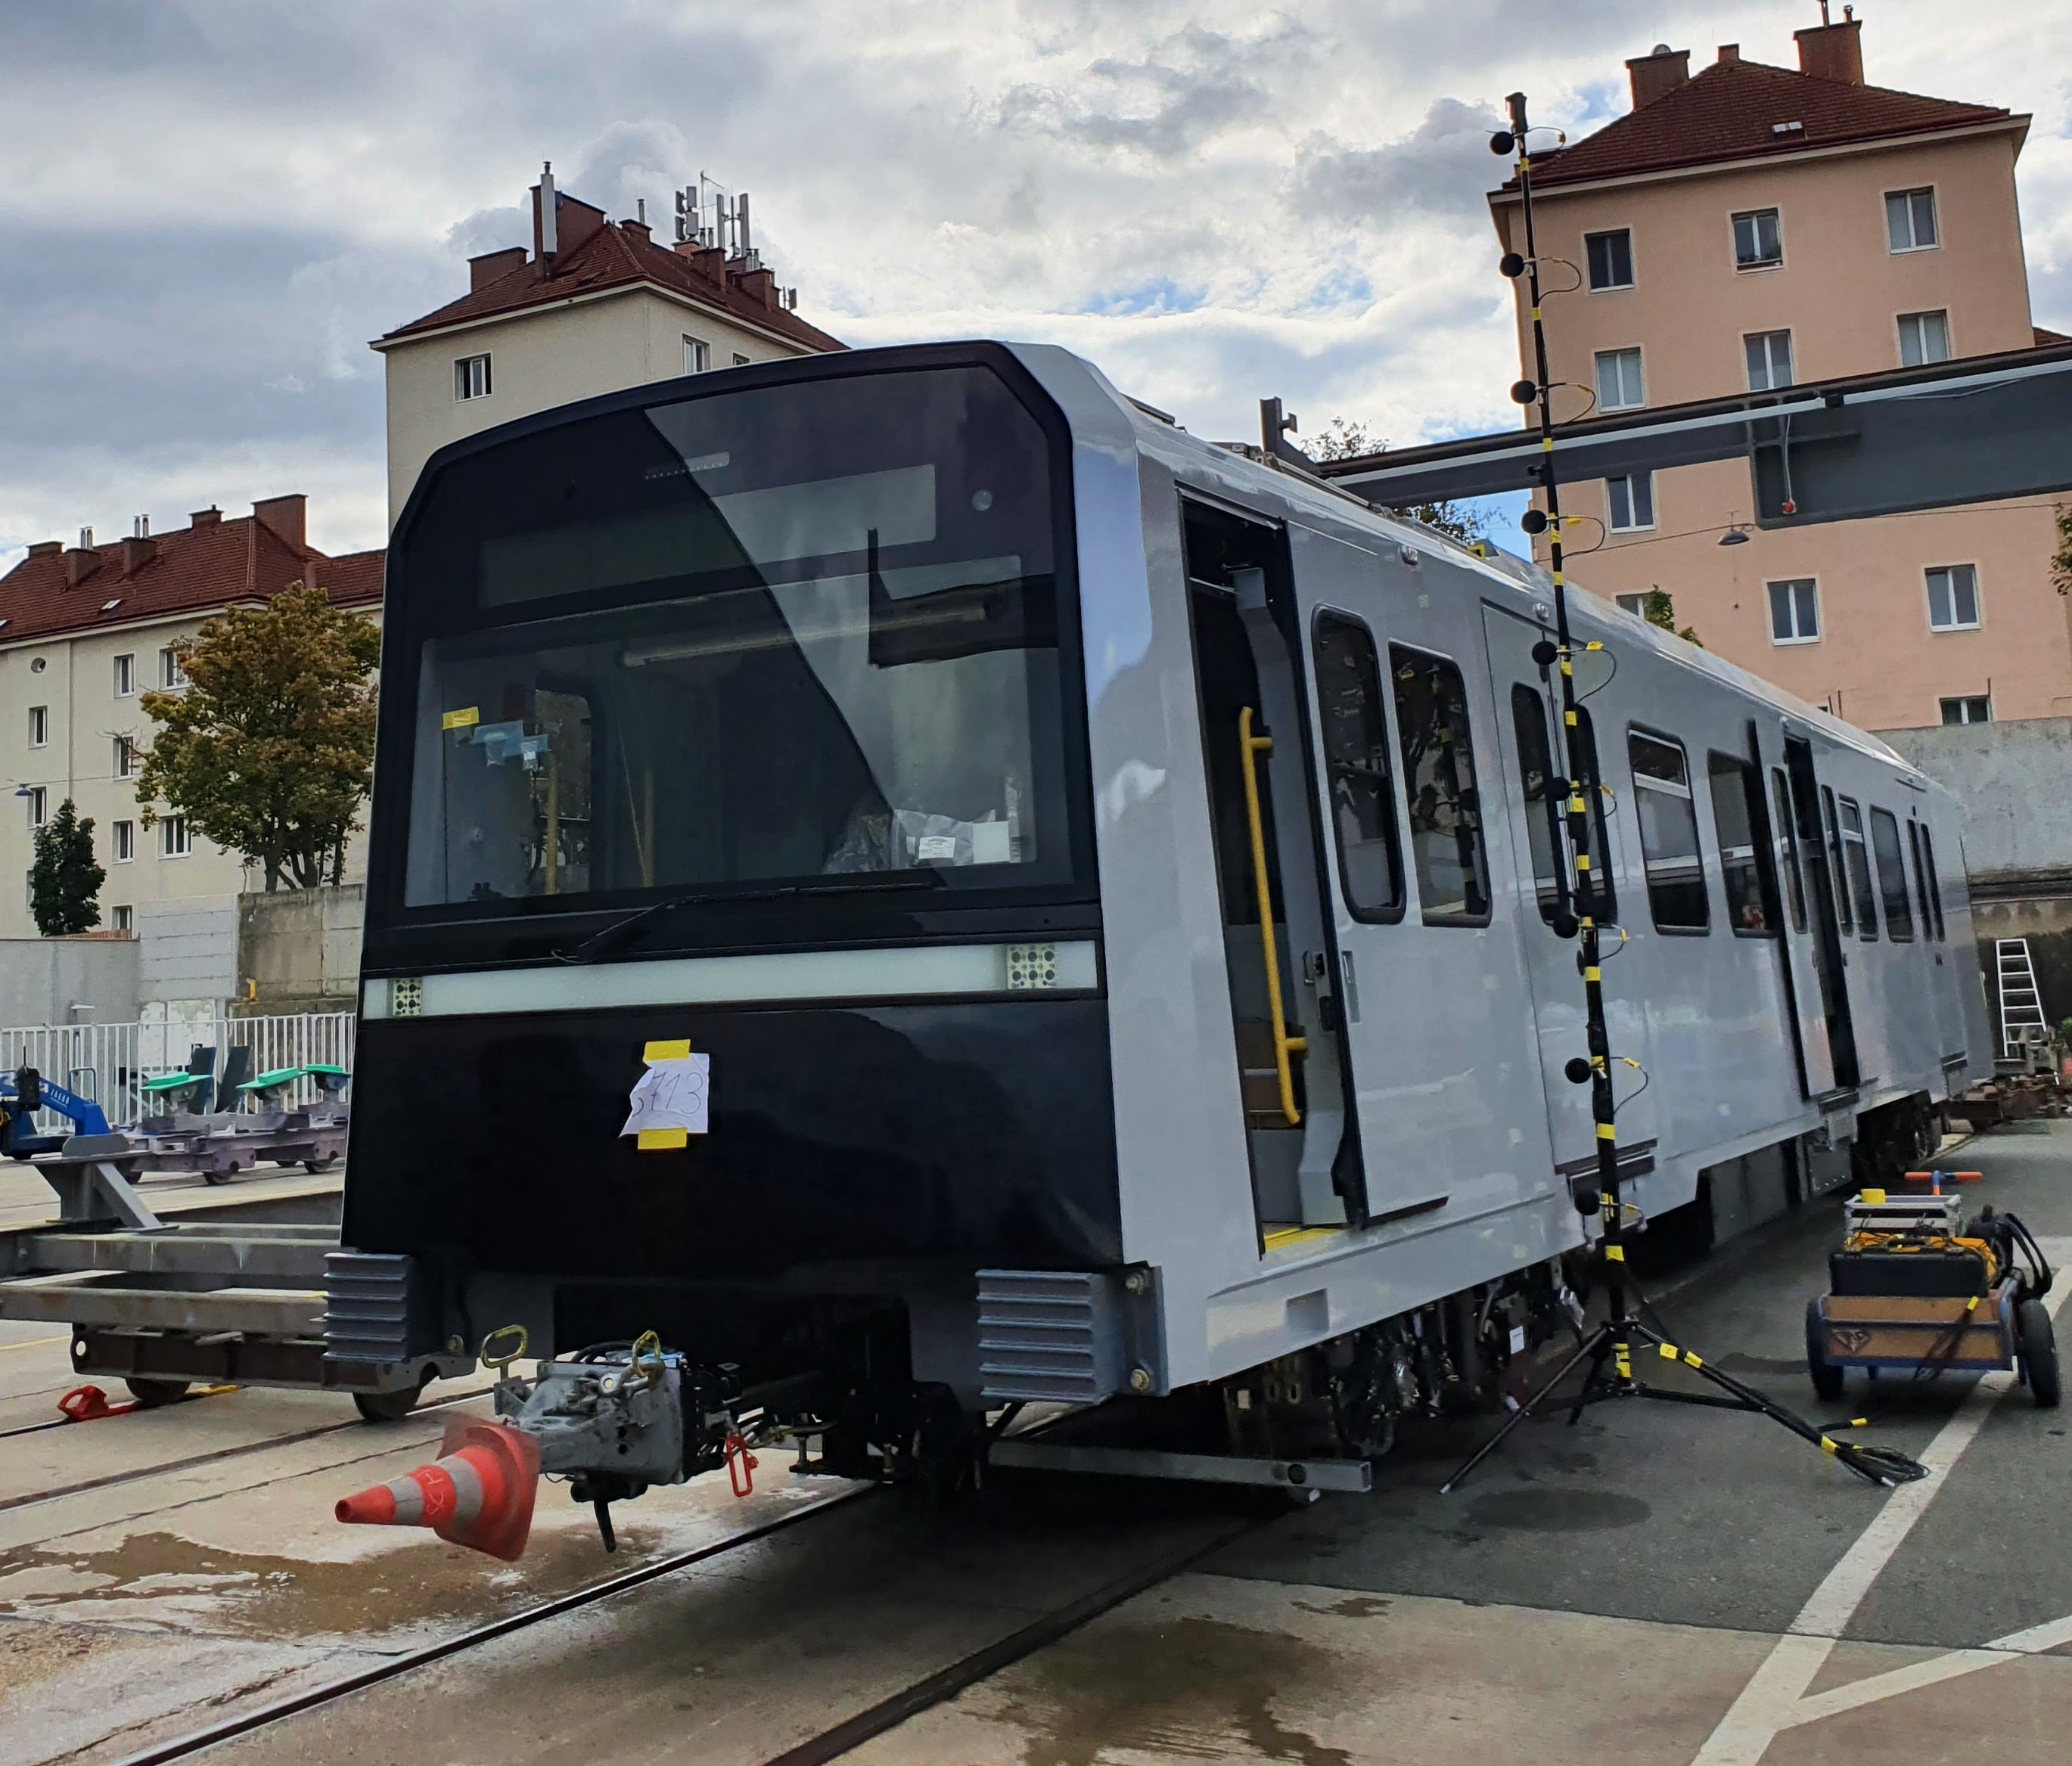
\includegraphics[width=\linewidth]{fig/Static_measurement_front_view.jpg}
         \caption{Front view}
         \label{fig:ubxfrontview}
     \end{subfigure}
     %\par\bigskip
     %\hspace{0.1\textwidth}
     %\hfill
\end{figure}

\begin{figure}[H]\ContinuedFloat
    \centering
    \begin{subfigure}[b]{\textwidth}
         \centering
         \includegraphics[width=\linewidth]{fig/Static_measurement_side_view.png}
         \caption{Side view}
         \label{fig:ubxsideview}
     \end{subfigure}
     \caption{Outer pressure field measurement setup.}
     \label{fig:outersetup}
\end{figure}

\begin{figure}[H]
     \centering
     \begin{subfigure}[b]{0.4\textwidth}
         \centering
         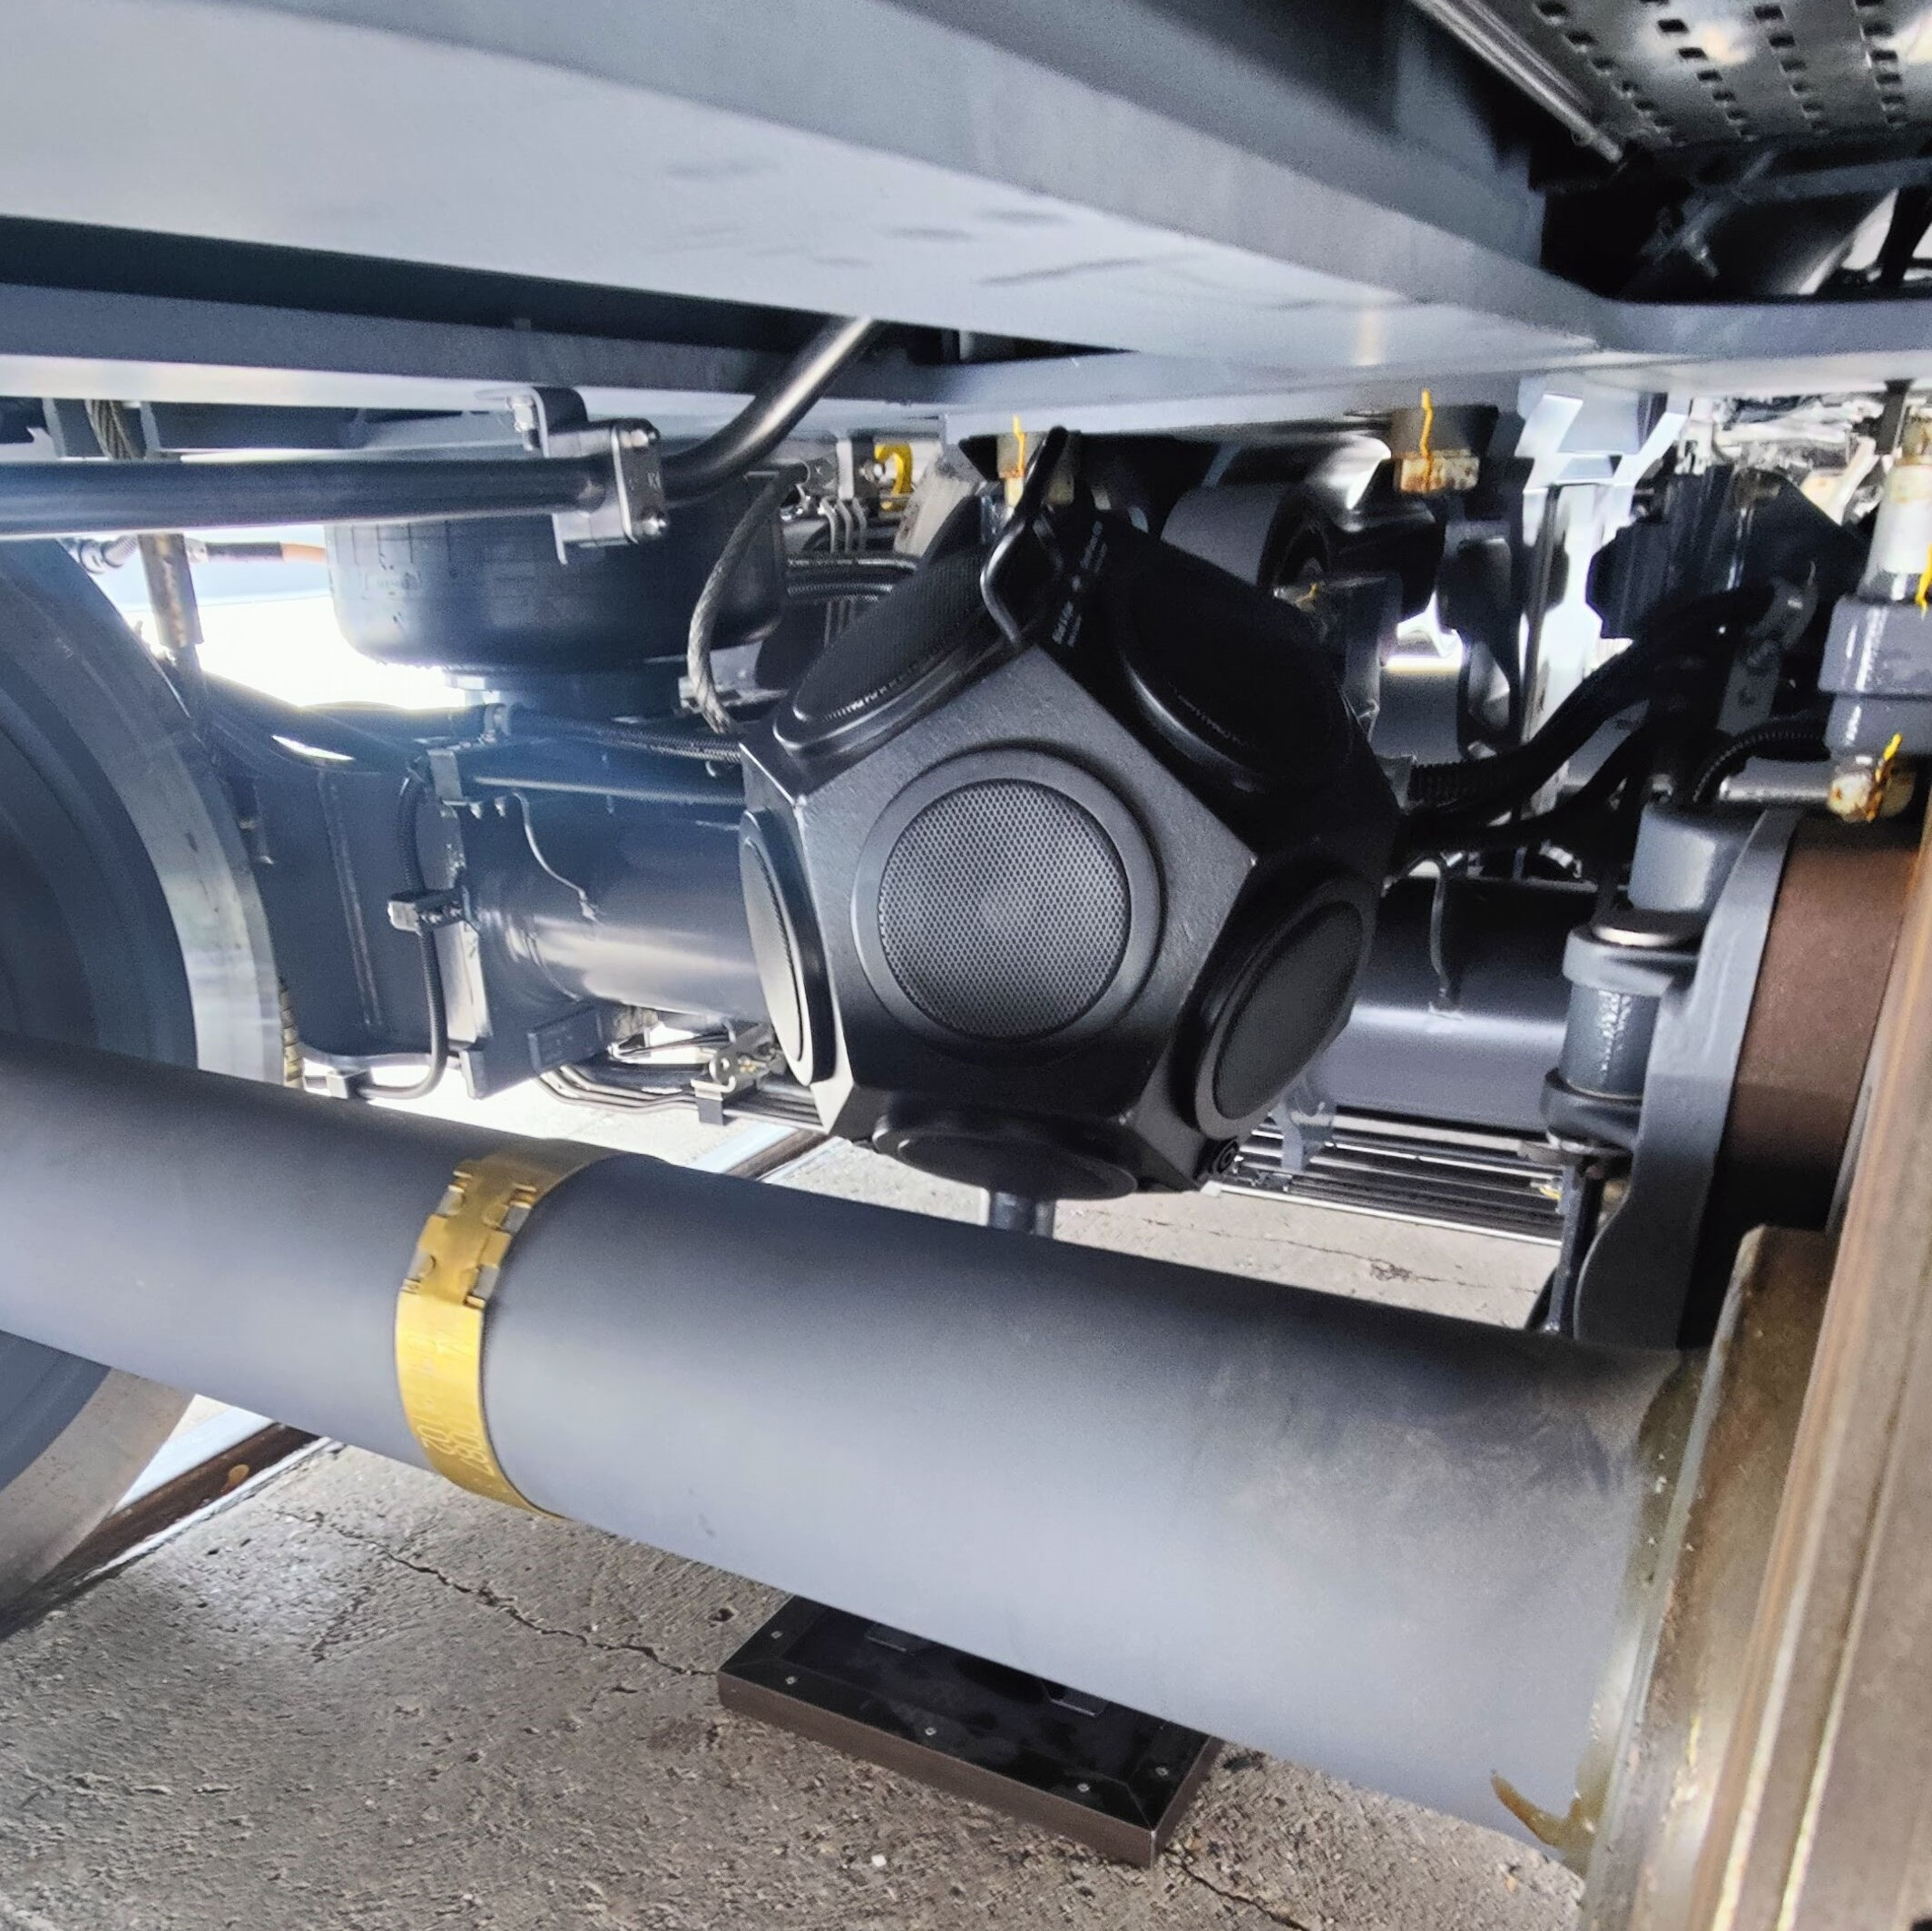
\includegraphics[width=\linewidth]{fig/loudspeaker_position_A.jpg}
         \caption{Position A: front of the bogie}
     \end{subfigure}
     %\par\bigskip
     \hspace{0.1\textwidth}
     %\hfill
     \begin{subfigure}[b]{0.4\textwidth}
         \centering
         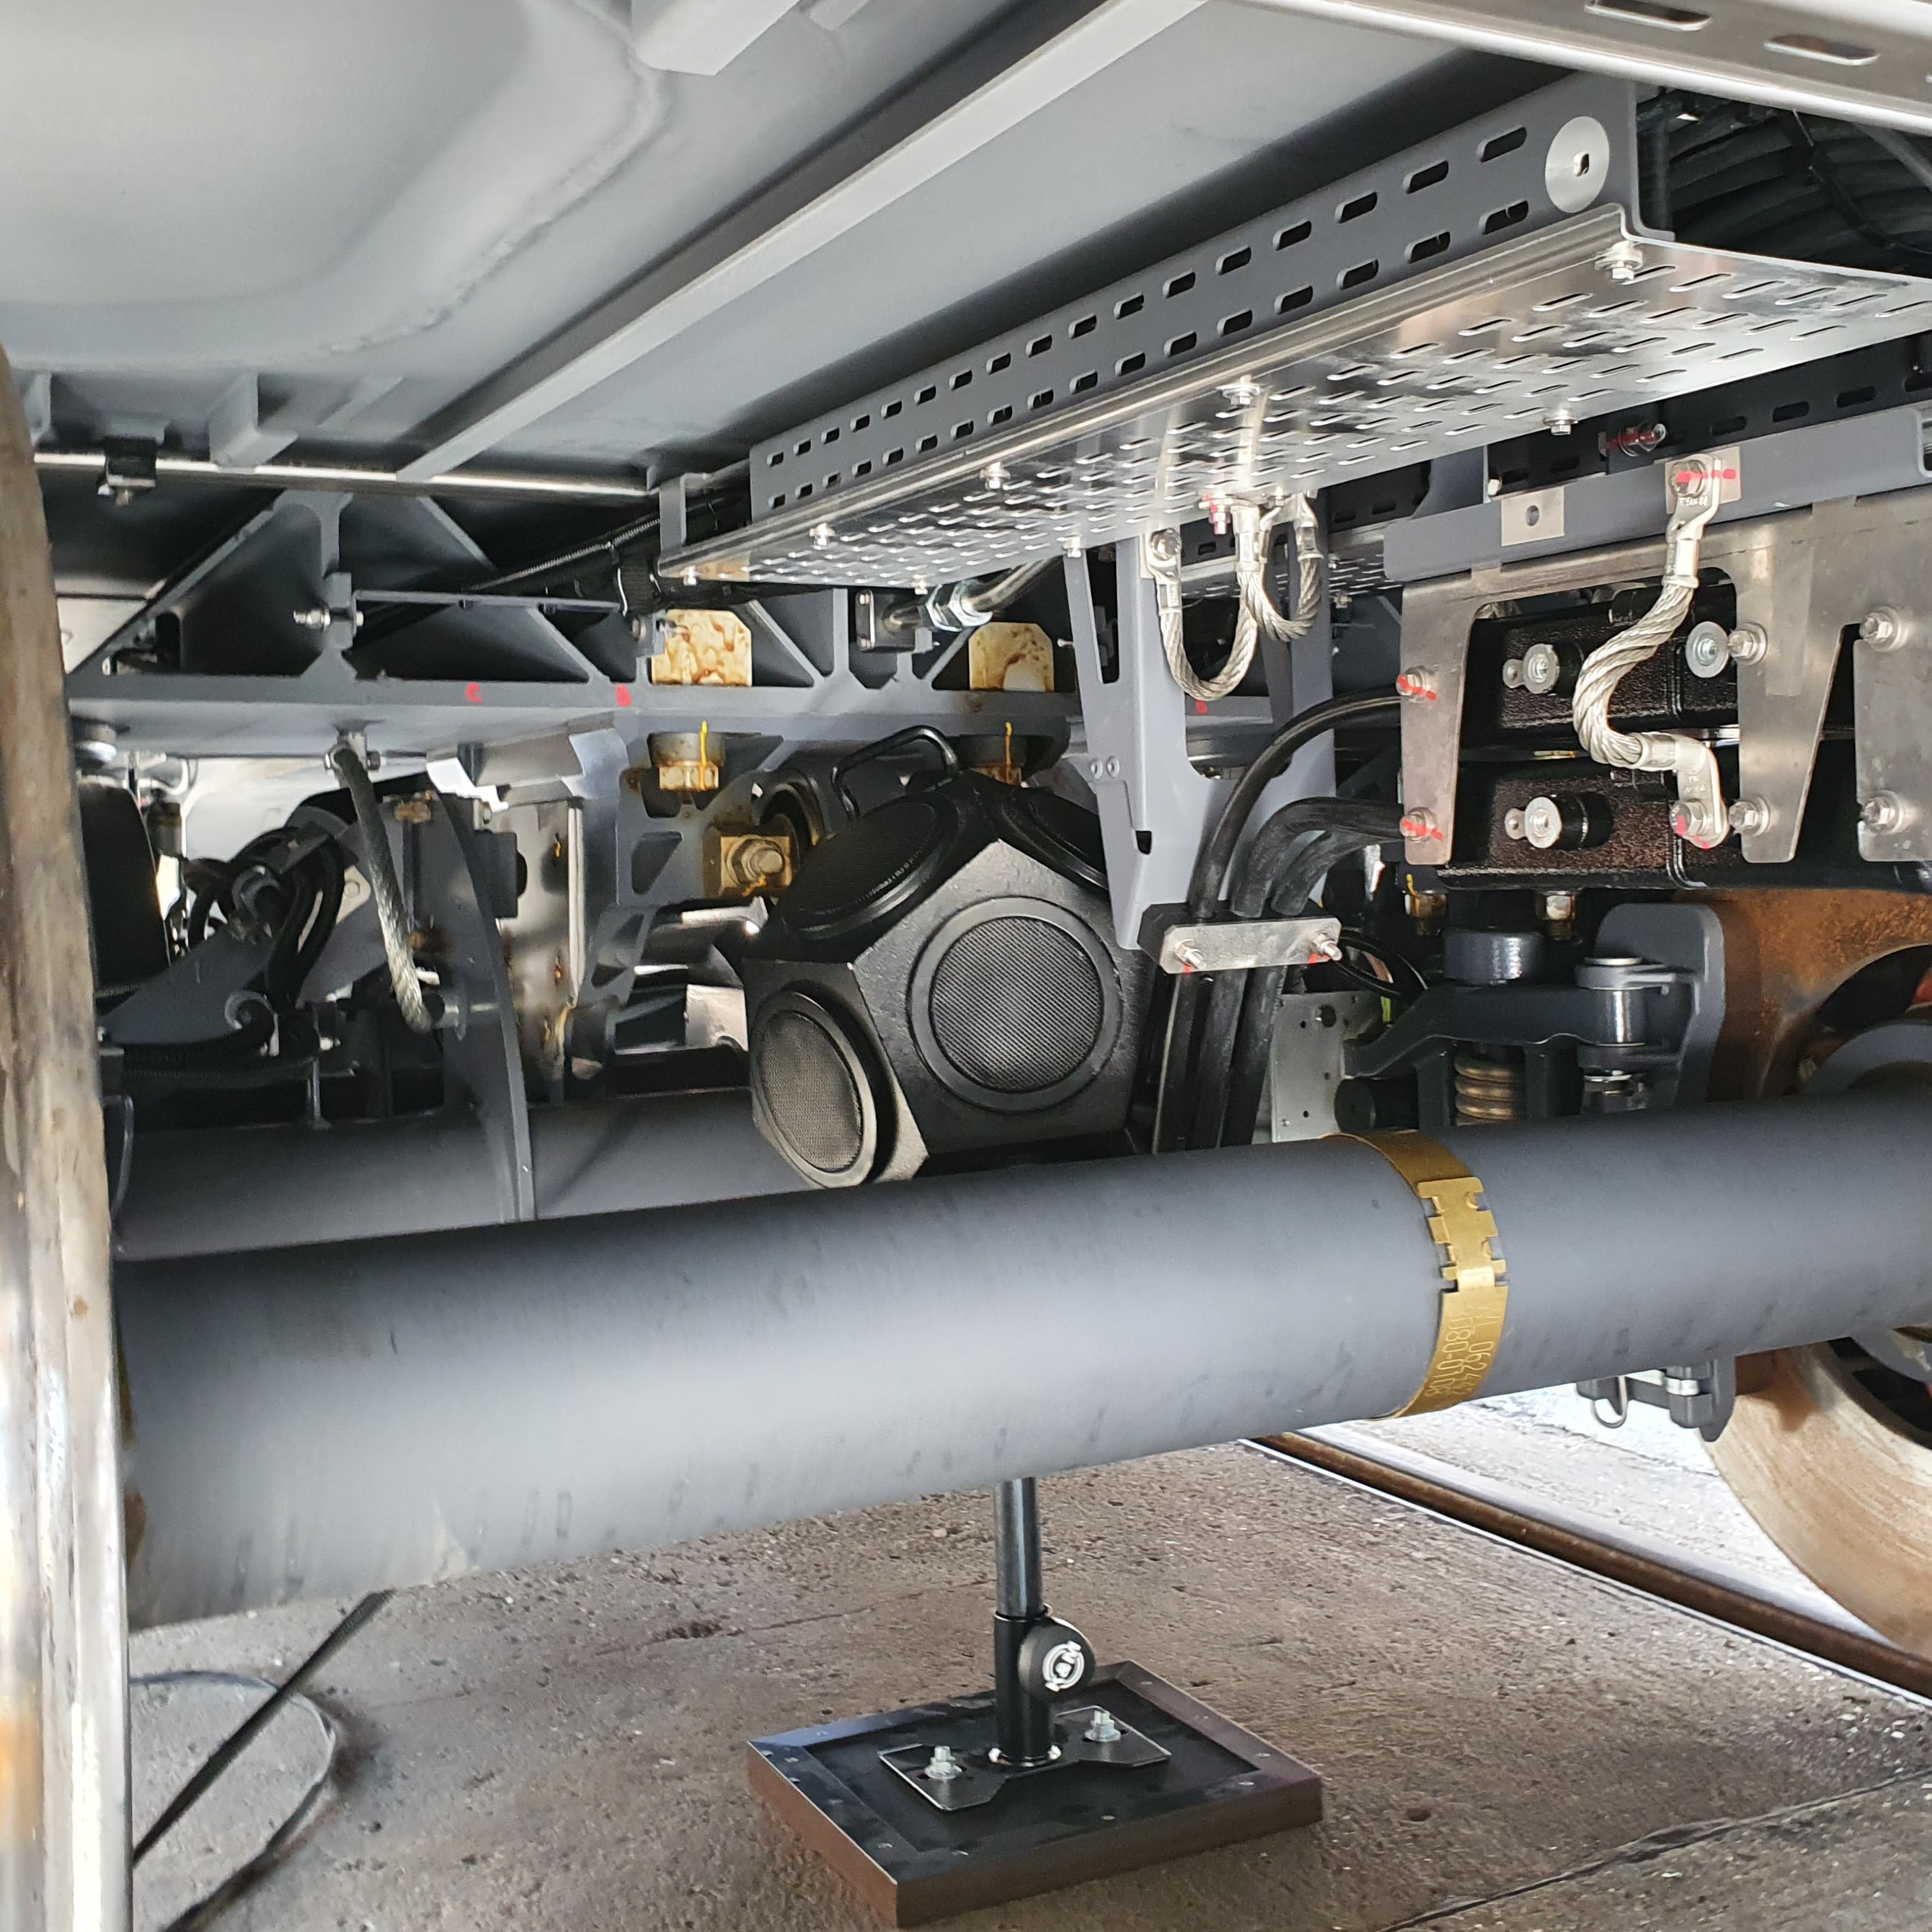
\includegraphics[width=\linewidth]{fig/loudspeaker_position_B.jpg}
         \caption{Position B: rear of the bogie}
     \end{subfigure}
     \caption{Loudspeaker locations.}
     \label{fig:loudspeakerposition}
\end{figure}

\begin{figure}[H]
     \centering
     \begin{subfigure}[b]{\textwidth}
         \centering
         \includegraphics[width=\linewidth]{fig/Measurement_positions.png}
         \caption{Measurement positions a to i}
     \end{subfigure}
     %\par\bigskip
     %\hspace{0.1\textwidth}
     %\hfill
\end{figure}

\begin{figure}[H]\ContinuedFloat
    \centering
    \begin{subfigure}[b]{0.6\textwidth}
         \centering
         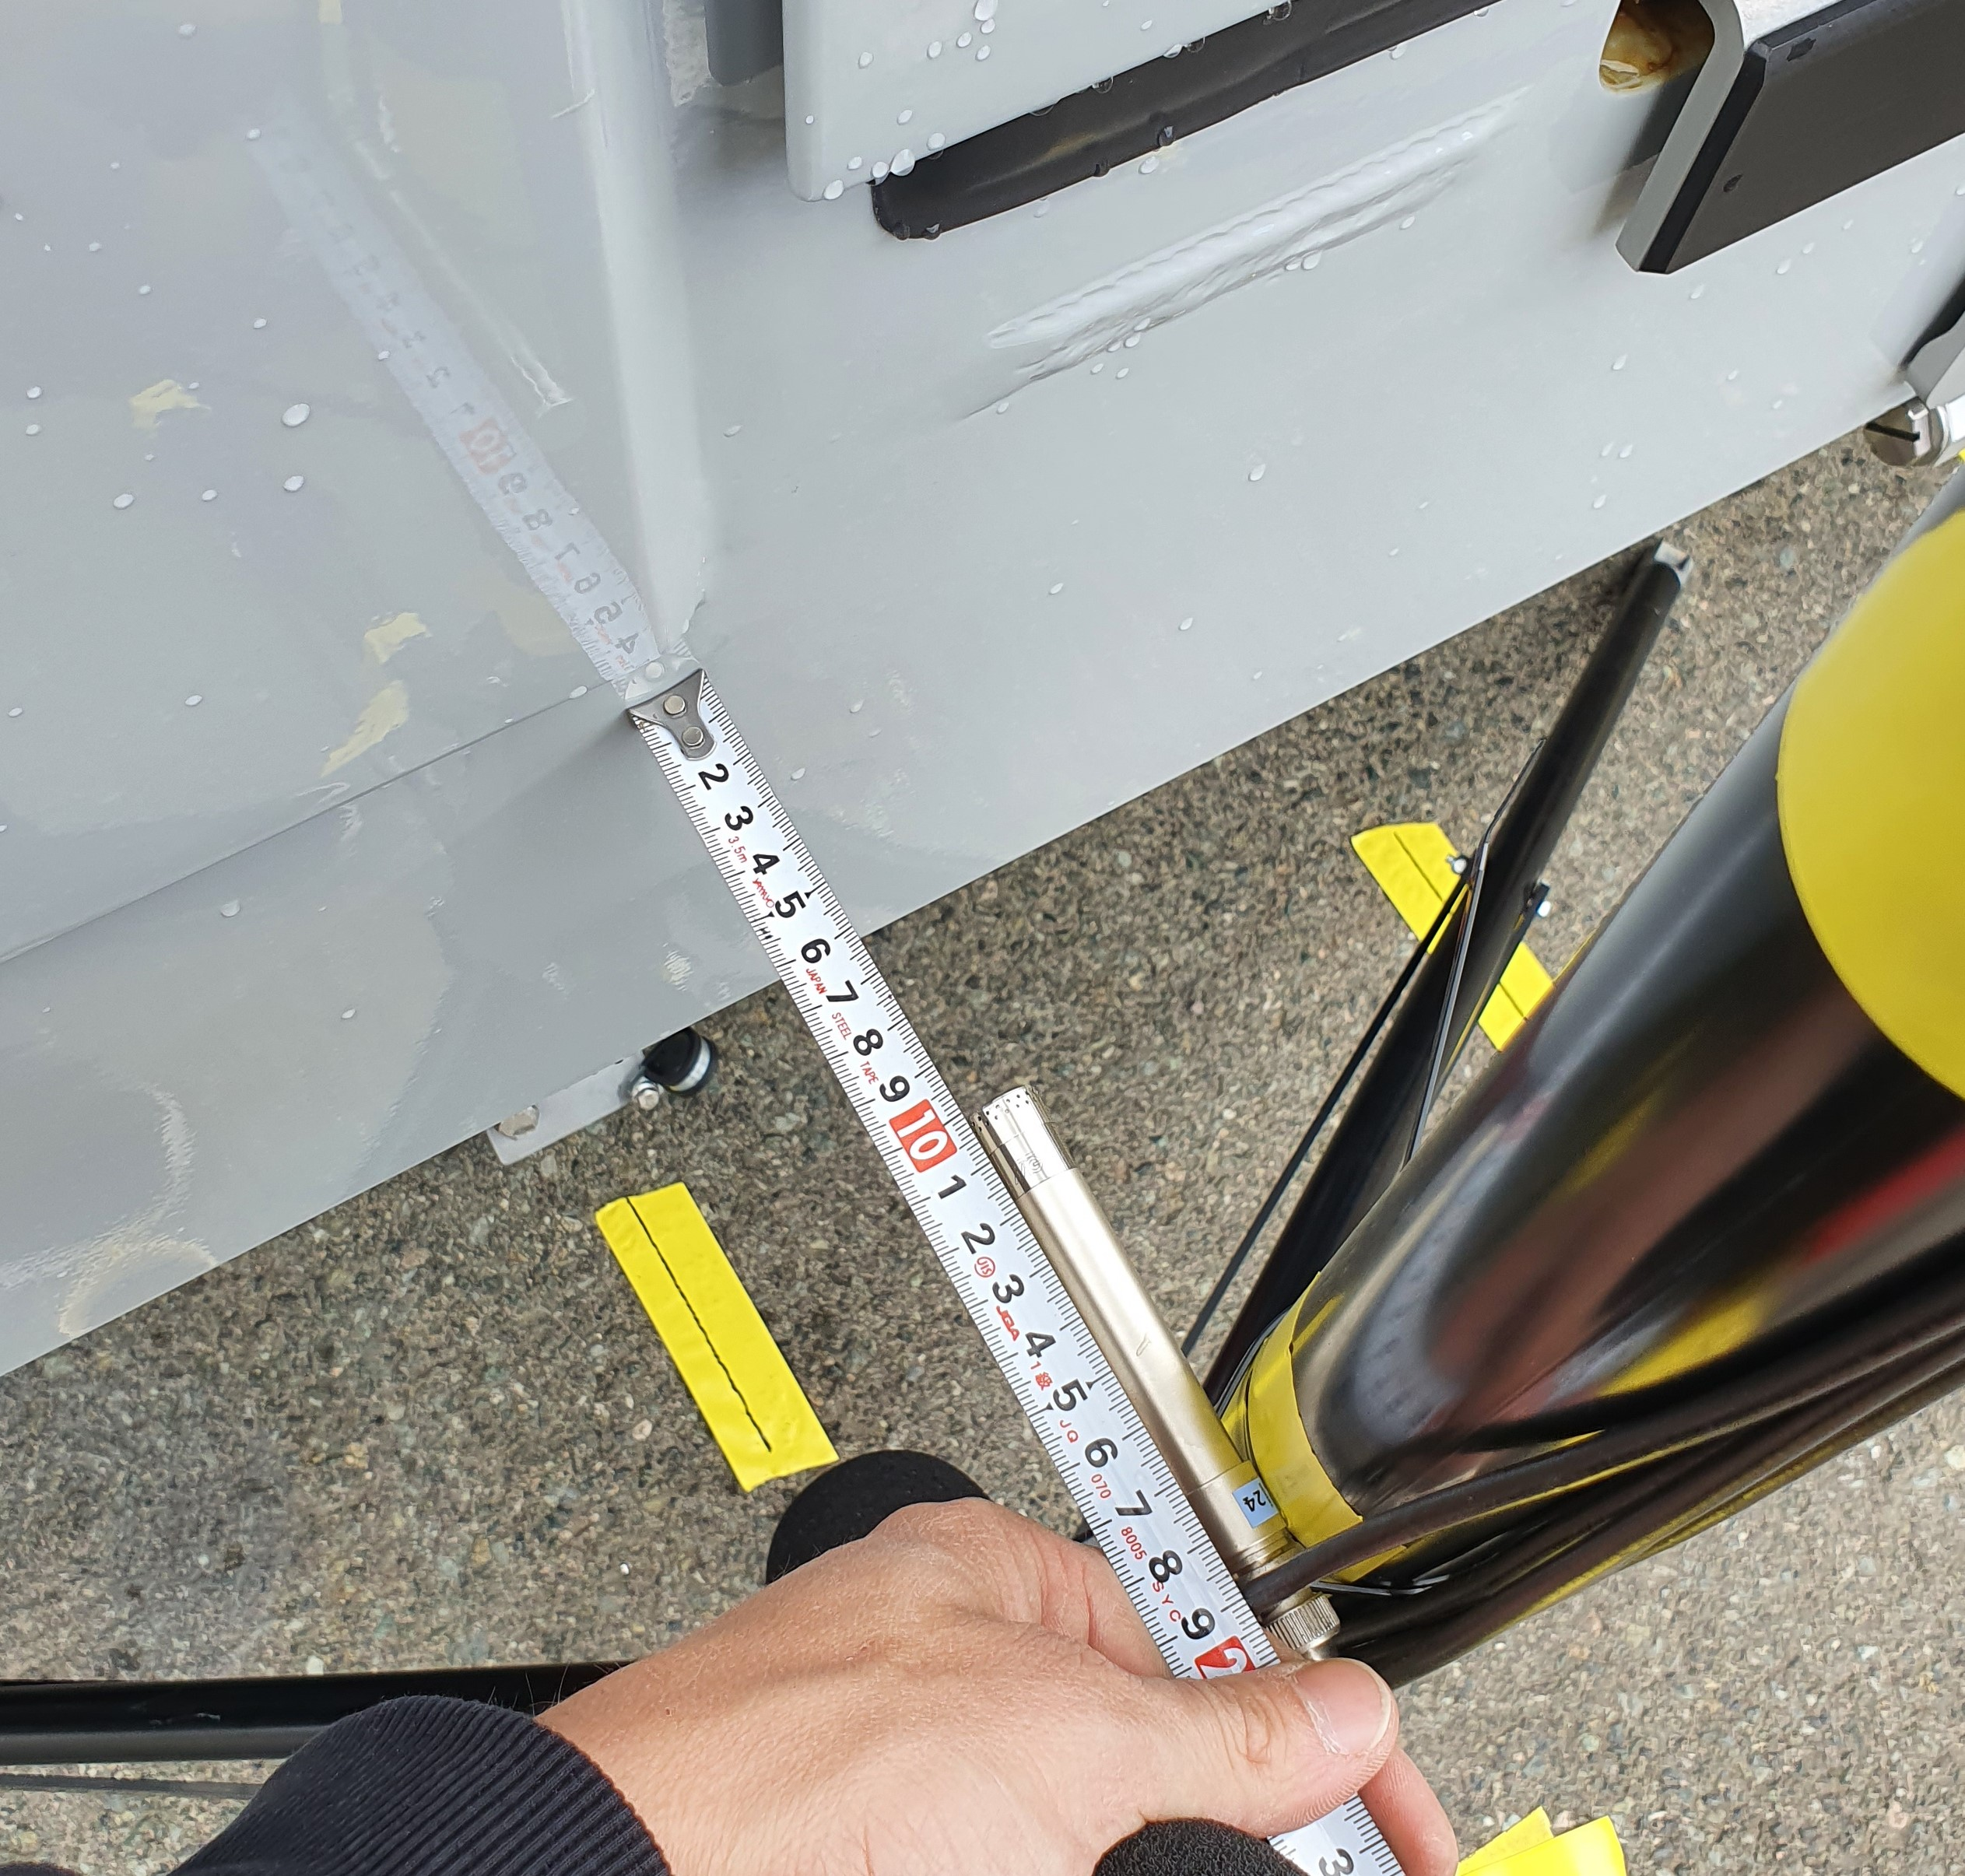
\includegraphics[width=\linewidth]{fig/position_of_microphones.jpg}
         \caption{Position a: centerline of the bogie, 10 cm away from carbody edge}
         \label{fig:position_a}
     \end{subfigure}
     \caption{Measurement positions of microphone array.}
     \label{fig:microphoneposition}
\end{figure}

\subsection*{Measurement results}

In \cref{fig:timedomain}, the measured time signal of microphone 1 (0.5 m above ground) at measurement position a (front bogie centerline, 10 cm away from car body) with loudspeaker placed at the front of the bogie are shown. The signal was converted into frequency domain using Fourier transformation as shown in \cref{fig:frequencydomain}. The post-processing was done directly in the provided software suit Müller-BBM PAK 6.x. \Cref{fig:fftparameter} shows a screenshot of the software GUI and the FFT parameters used are circled.

In \cref{fig:frequencydomain}, the blue curve shows the amplitude of acoustic pressure in narrow band resolution. The narrow band data was converted to 1/n octave form by summing up the amplitude of narrow-band spectral lines contained within the corresponding frequency bandwidth. The advantage of post-processing the data into octave bands is that it provides clearer information about the frequency composition of the noise signal. For example, it can be observed that in the 1/3 octave curve in \cref{fig:frequencydomain}, the peak of the SPL appears at 315 Hz, which also matches the peak in the SWL spectrum of the sound source as shown in \cref{fig:average_SWL}.

\begin{figure}[H]
    \centering
    \begin{subfigure}[b]{0.48\textwidth}
        \centering
        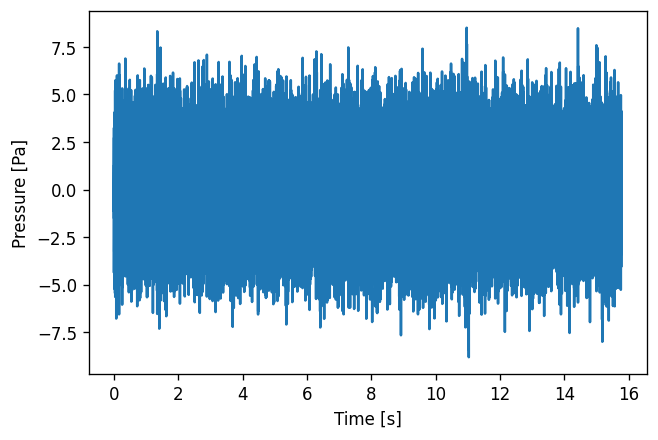
\includegraphics{fig/time_signal.png}
        \caption{Time domain}
        \label{fig:timedomain}
    \end{subfigure}
    \begin{subfigure}[b]{0.48\textwidth}
        \centering
        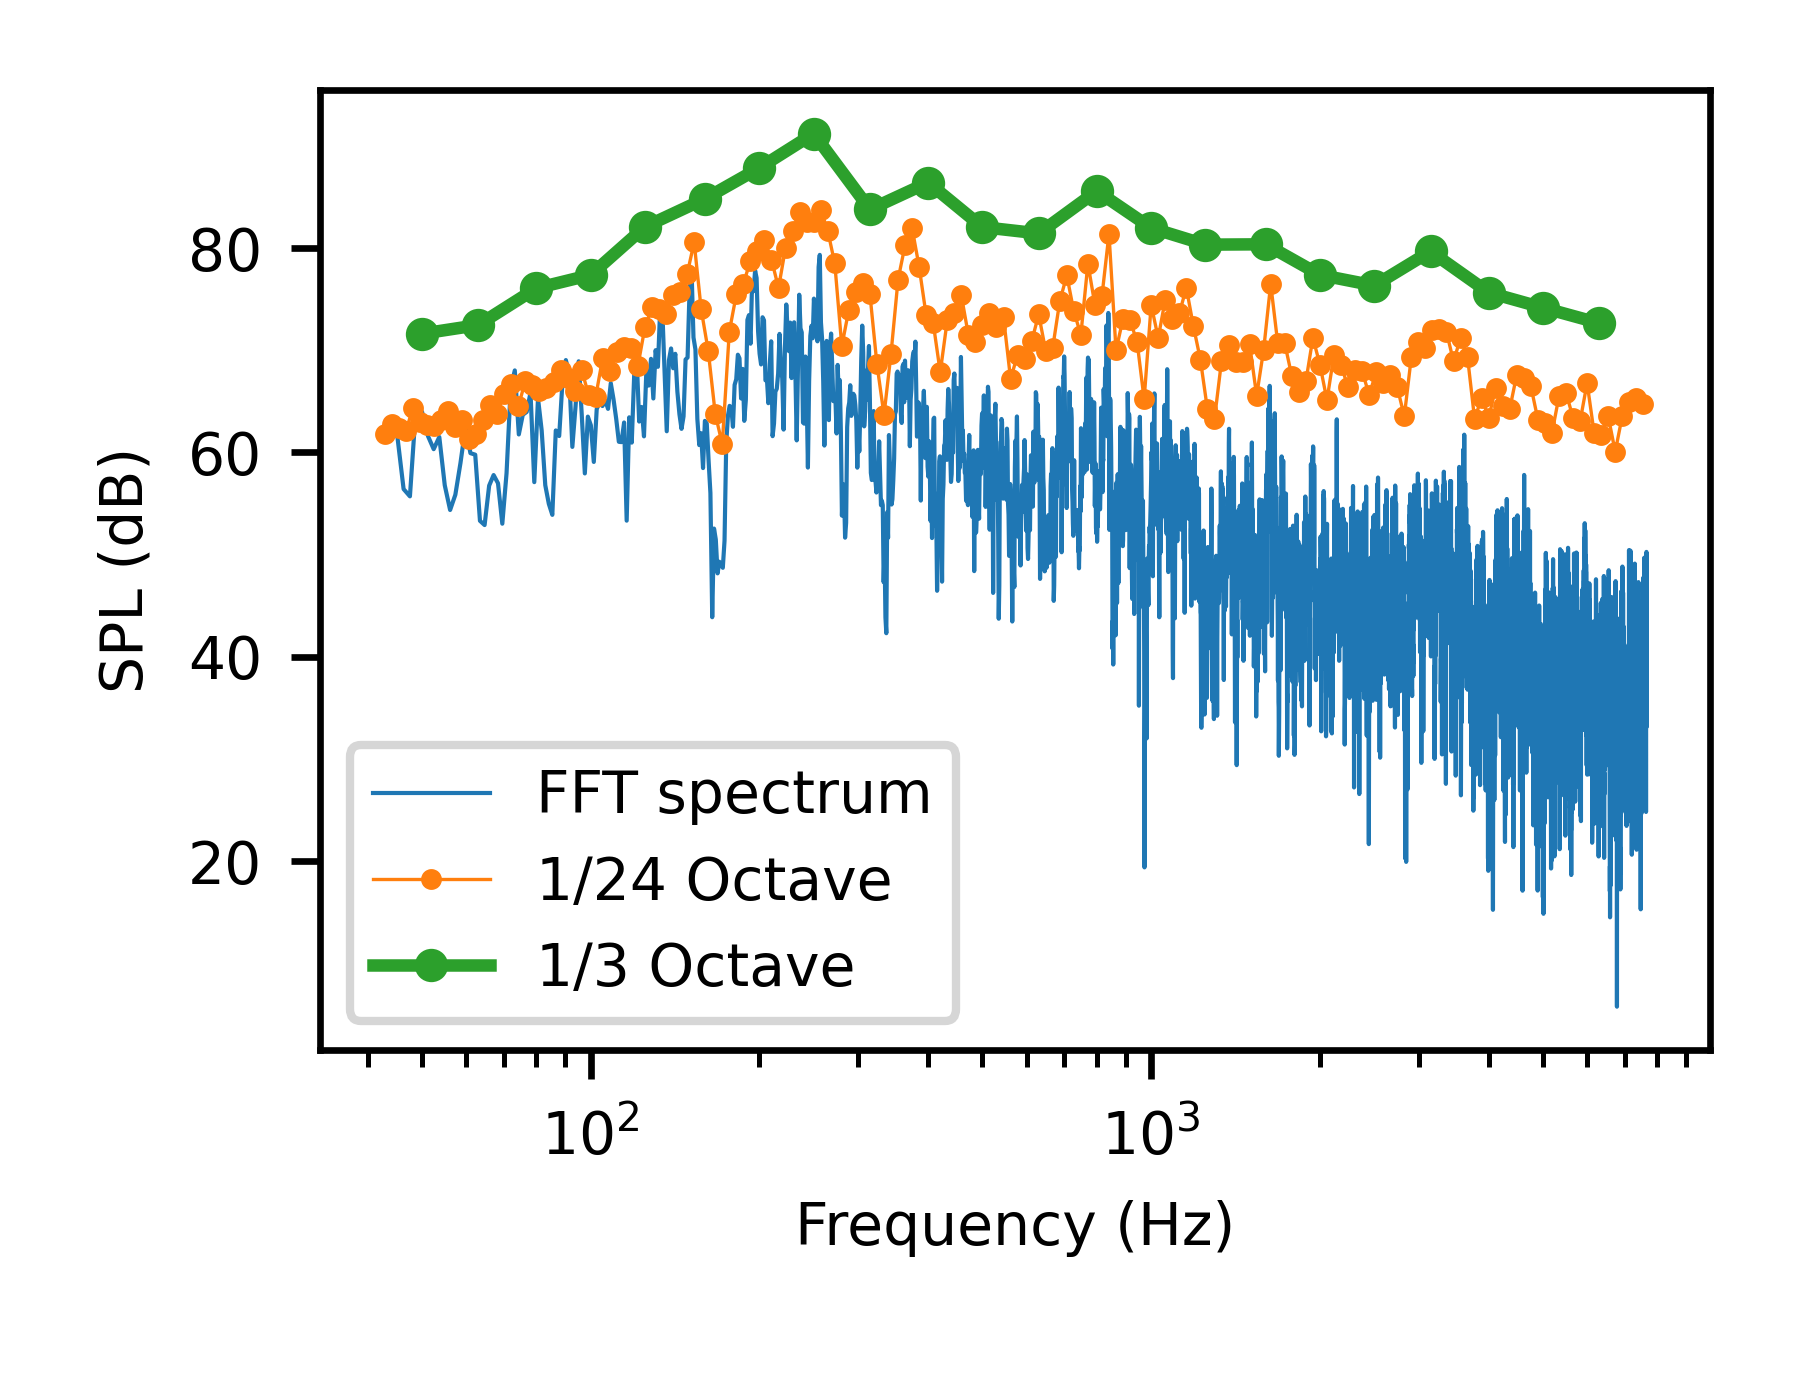
\includegraphics{fig/fft_spectra.png}
        \caption{Frequency domain}
        \label{fig:frequencydomain}
    \end{subfigure}
    
    \caption{Measurement data at measurement position a, at \SI{0.5}{\meter} height above ground, loudspeaker located at the front of the bogie.}
    \label{fig:measurementsignal}
\end{figure}

\begin{figure}[H]
    \centering
    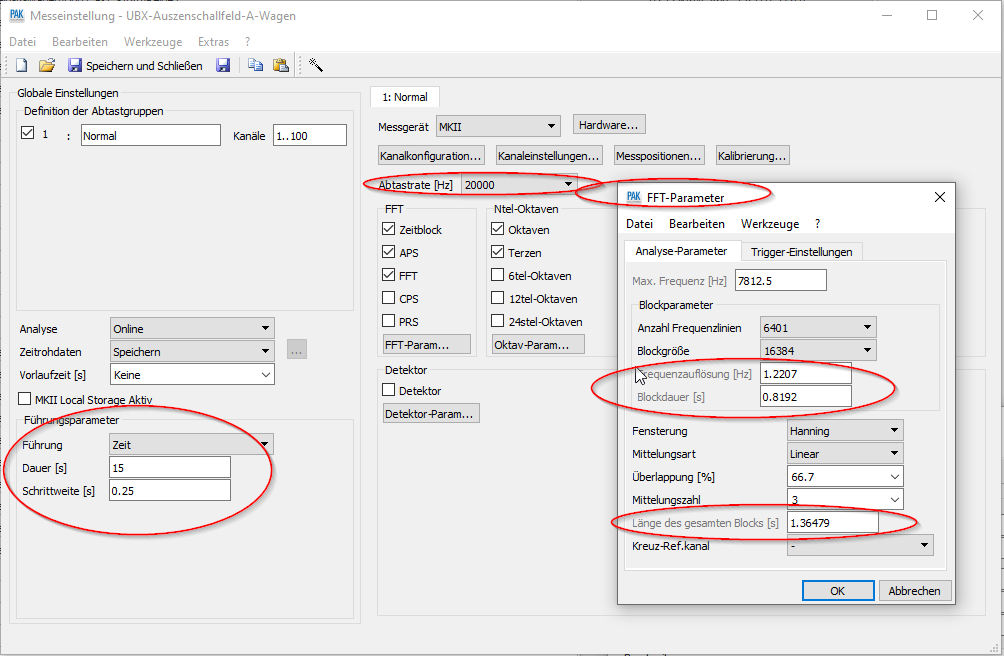
\includegraphics[width=\linewidth]{fig/fft_parameter.png}
    \caption{GUI of the Müller-BBM PAK software and FFT parameters used.}
    \label{fig:fftparameter}
\end{figure}

\begin{figure}[H]
    \centering
     \begin{subfigure}[b]{0.49\textwidth}
        \centering
        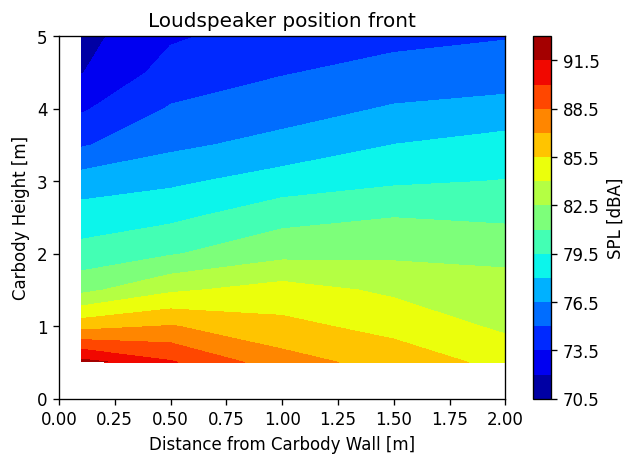
\includegraphics[width=\textwidth]{fig/pressure_field_loudspeaker_front.png}
        \caption{Loudspeaker position front}
    \end{subfigure}
    \begin{subfigure}[b]{0.49\textwidth}
        \centering
        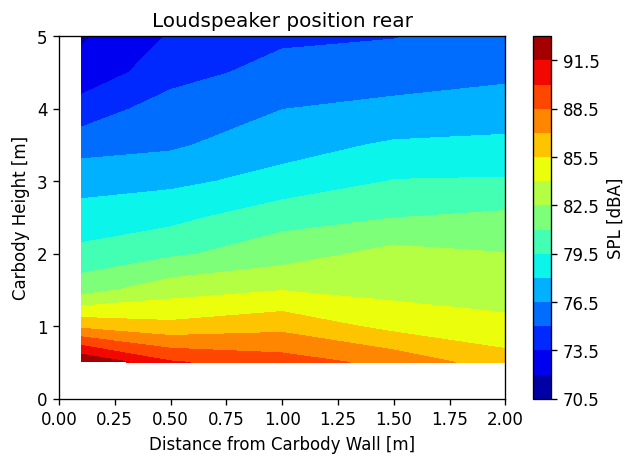
\includegraphics[width=\textwidth]{fig/pressure_field_loudspeaker_rear.png}
        \caption{Loudspeaker position rear}
    \end{subfigure}
        \caption{Pressure field around car body.}
        \label{fig:pressurefield}
\end{figure}

\noindent In \cref{fig:pressurefield}, a visualization of the total pressure field around the carbody is shown. The horizontal axis represents the distance from carbody wall, the vertical axis the height above ground and the color the overall A-weighted pressure level, respectively. The white space in the plot is due to the missing data in the measurement since the measurement positions start at 10 cm away from carbody wall and half meter above ground. Comparing the pressure field of the two different loudspeaker locations, the asymmetric effect introduced by the brake disc can be observed. The brake disc of the front wheel axle standing in the transmission path of the loudspeaker seems to block a part of the acoustic wave.

\begin{figure}[H]
    \centering
     \begin{subfigure}[b]{0.48\textwidth}
        \centering
        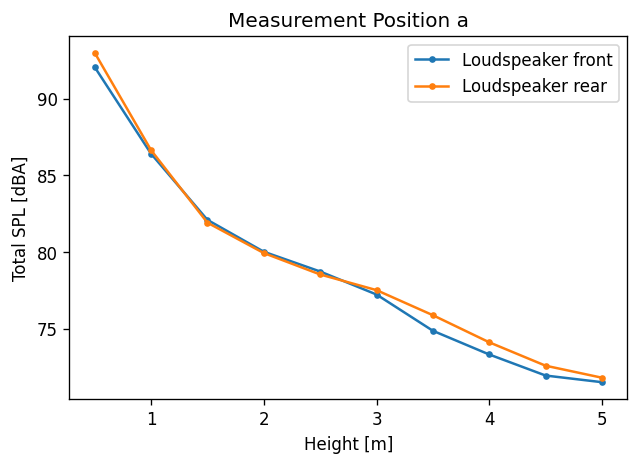
\includegraphics{fig/pressure_over_height_pos_a.png}
        \caption{Measurement position a}
        \label{fig:SPLoverheight_pos_a}
    \end{subfigure}
    \begin{subfigure}[b]{0.48\textwidth}
        \centering
        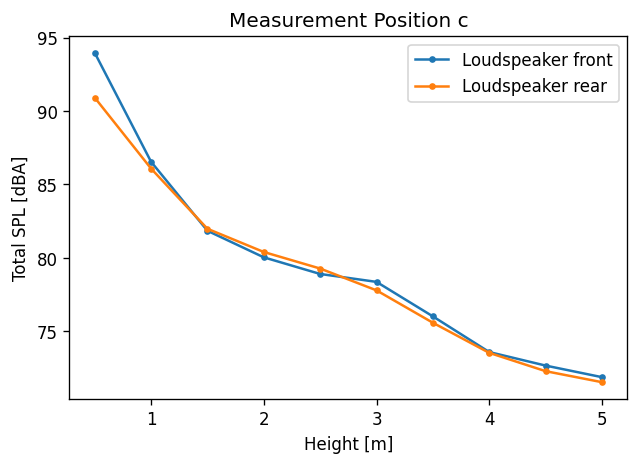
\includegraphics{fig/pressure_over_height_pos_c.png}
        \caption{Measurement position c}
        %\label{fig:frequencydomain}
    \end{subfigure}
    \caption{Overall A-weighted sound pressure level at example measurement positions.}
    \label{fig:SPLoverheight}
\end{figure}

\noindent In order to compare the pressure field quantitatively, one can plot the acoustic pressure as function of height for different measurement positions, which can be seen in the figures above. In \ref{fig:SPLoverheight_pos_a} it can be observed that at measurement position a, the pressure curve caused by loudspeaker at different locations shares similar shape, and the pressure is strictly decreasing over carbody height.

\begin{figure}[H]
    \centering
     \begin{subfigure}[b]{0.48\textwidth}
        \centering
        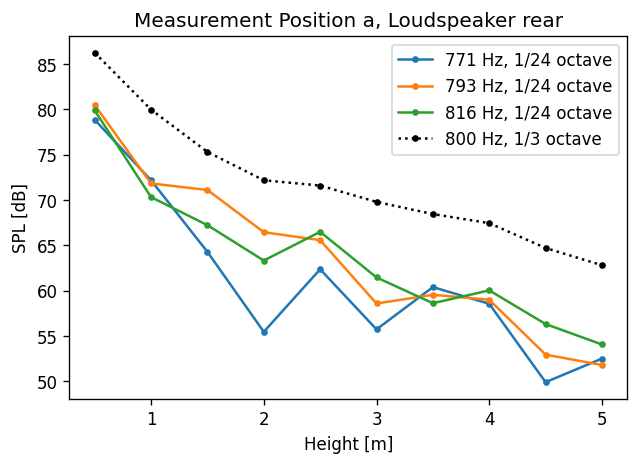
\includegraphics{fig/pressure_over_height_800Hz.png}
        \caption{800 Hz}
        \label{fig:SPLoverheight_frequency_800Hz}
    \end{subfigure}
    \begin{subfigure}[b]{0.48\textwidth}
        \centering
        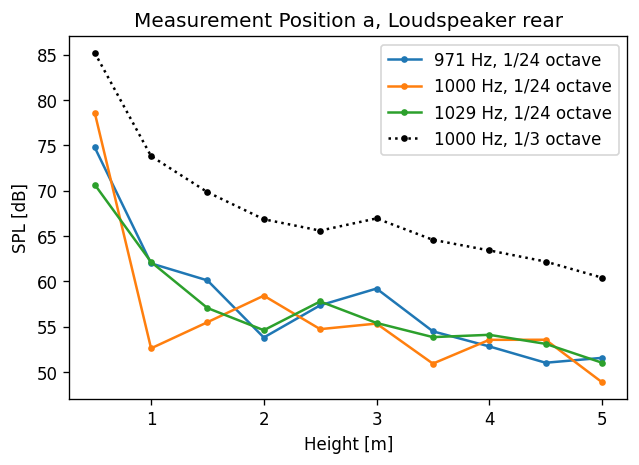
\includegraphics{fig/pressure_over_height_1000Hz.png}
        \caption{1000 Hz}
        \label{fig:SPLoverheight_frequency_1000Hz}
    \end{subfigure}
    \caption{SPL distribution of example third octave bands at measurement position a with loudspeaker at the rear. Solid line: 1/24-octave center frequency. Dashed line: 1/3-octave center frequency.}
    \label{fig:SPLoverheight_frequency}
\end{figure}

\noindent In Fig. \ref{fig:SPLoverheight_frequency}, the sound pressure level over height for different 1/n octave band center frequencies is displayed. In the 1/24 octave resolution, several local minima in the curve shape can be observed, e.g., for 771 Hz in fig. \ref{fig:SPLoverheight_frequency_800Hz} or for 1000 Hz in Fig. \ref{fig:SPLoverheight_frequency_1000Hz}, which are caused by the destructive interference of the acoustic wave. The destructive interference can also be observed in the pressure field of the single frequency band as shown in Fig. \ref{fig:pressurefield_1000Hz}, sinks in acoustic field are to be found at about 1 m and 3.5 m height, respectively, which correspond to the position of the local minima in Fig. \ref{fig:SPLoverheight_frequency_1000Hz}.

\begin{figure}[H]
    \centering
    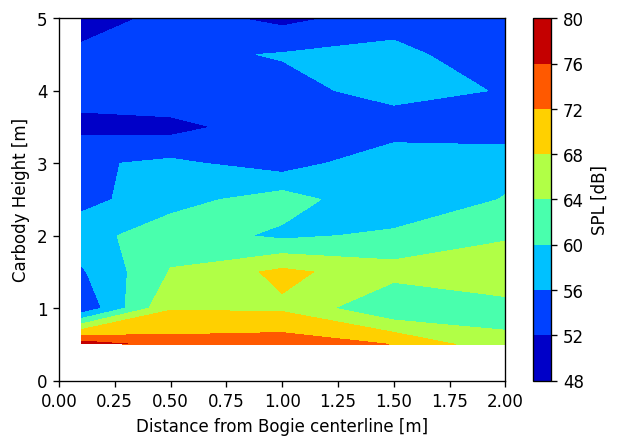
\includegraphics[width=0.6\linewidth]{fig/pressure_field_1000Hz.png}
    \caption{Pressure field of 1/24-octave frequency 1000 Hz with loudspeaker placed at the rear.}
    \label{fig:pressurefield_1000Hz}
\end{figure}


\chapter{Finite Element Modeling}
\label{chap:FEM}

In this chapter, the development of the finite element model of the UBX metro and the simulation setup are described. First, in section \ref{section:geometry}, the design of the model geometry and the mesh of the model are shown. Then, in section \ref{section:boundary_conditions}, the incorporation of boundary conditions into the finite element model is described. Finally, in section \ref{section:parametric_study}, a parametric study is carried out to investigate the influence of different simulation parameters on the solution of the initial finite element model. All these simulations are done with the acoustics module of the open-source FEM software openCFS \cite{opencfs}.


\section{Geometry and mesh}
\label{section:geometry}

As shown in sec. \ref{section:ubx_geometry}
Due to the large dimension of the car body 

a representative model has to be

\begin{figure}[H]
	\centering
	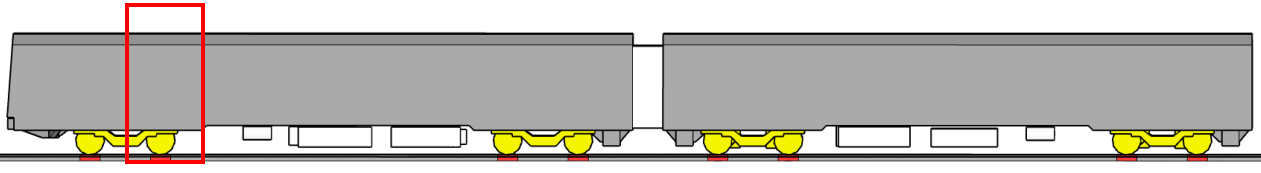
\includegraphics[width=\textwidth]{fig/chap4/geometry/model_area.png}
	\caption{Side view of UBX, red box marked the modeling area}
\end{figure}

\begin{figure}[H]
	\centering
	\begin{subfigure}[b]{0.4\textwidth}
		\centering
		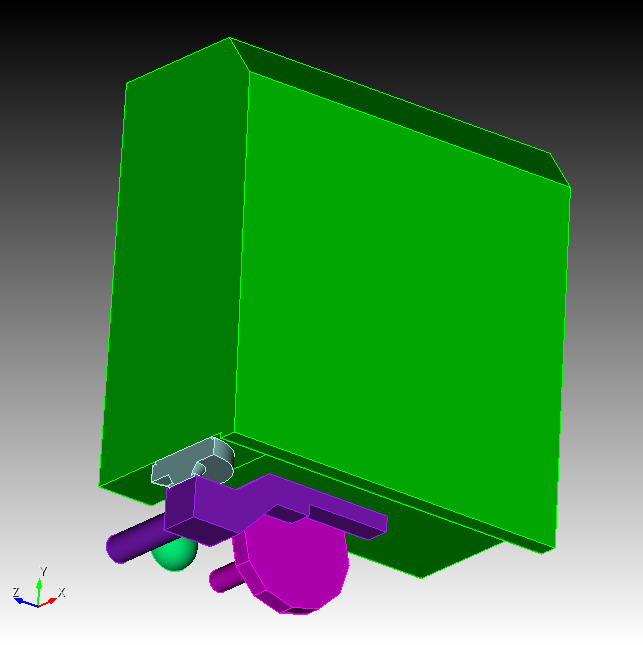
\includegraphics[width=0.9\linewidth]{fig/chap4/geometry/one_fourth_model.png}
		\caption{quarter model}
	\end{subfigure}
	\hfill
	\begin{subfigure}[b]{0.4\textwidth}
		\centering
		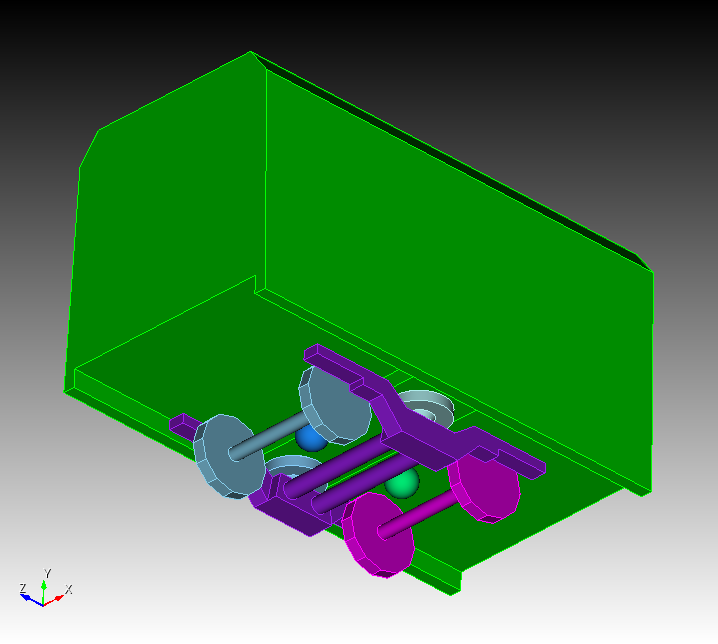
\includegraphics[width=\linewidth]{fig/chap4/geometry/initial_model_2.png}
		\caption{full model}
	\end{subfigure}
	\caption{Geometry of model}
\end{figure}



\subsection{Determination of simulation domain}
\subsection{Computational Effort}
The aim of this section is 

\section{Boundary conditions and loads}
\label{section:boundary_conditions}
\subsection{Modeling of sound source}

\section{General simulation setup}

\section{Parametric study}
\label{section:parametric_study}
\subsection{Variation of underfloor geometry}

\begin{figure}[H]
	\centering
	\begin{subfigure}[b]{0.49\textwidth}
		\centering
		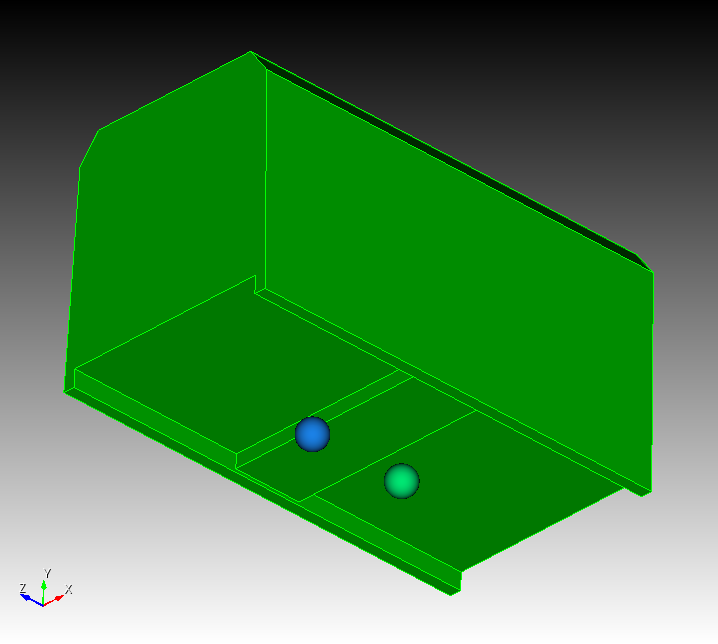
\includegraphics[width = 0.8\linewidth]{fig/chap4/geometry/no_underfloor_components_2.png}
		\caption{No underfloor components}
	\end{subfigure}
	\begin{subfigure}[b]{0.49\textwidth}
		\centering
		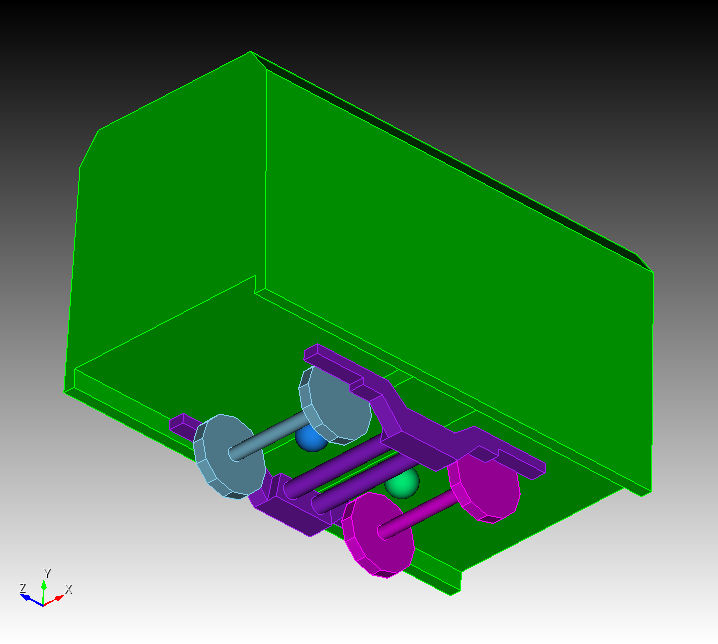
\includegraphics[width = 0.8\linewidth]{fig/chap4/geometry/no_air_suspension_2.png}
		\caption{No air suspension}
	\end{subfigure}
	\begin{subfigure}[b]{0.49\textwidth}
		\centering
		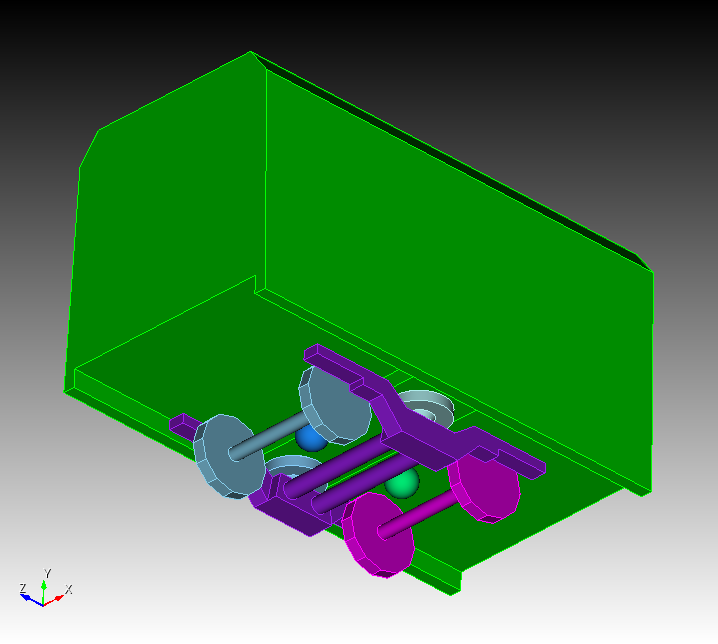
\includegraphics[width = 0.8\linewidth]{fig/chap4/geometry/initial_model_2.png}
		\caption{Initial model}
	\end{subfigure}
	\begin{subfigure}[b]{0.49\textwidth}
		\centering
		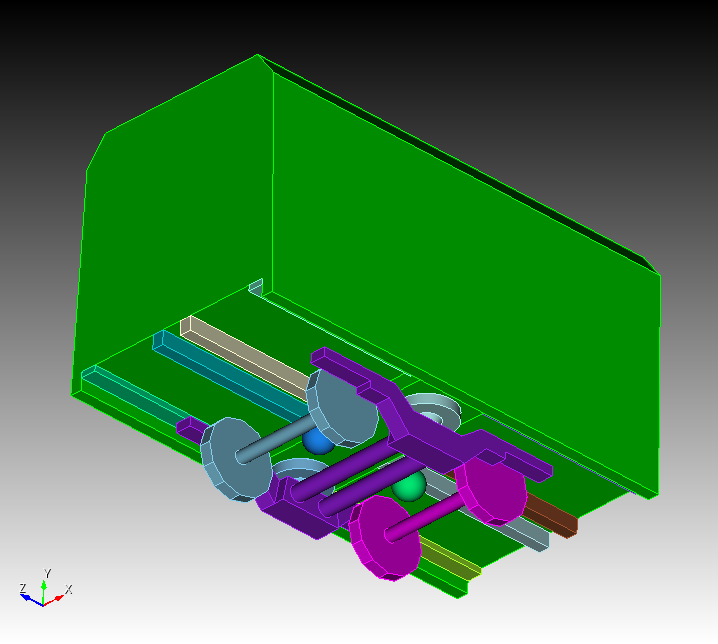
\includegraphics[width = 0.8\linewidth]{fig/chap4/geometry/additional_structures.png}
		\caption{Additional structures}
	\end{subfigure}

	\caption{Used geometry}
\end{figure}

\subsection{Inclusion of ground absorption}

\begin{figure}[H]
	\centering
	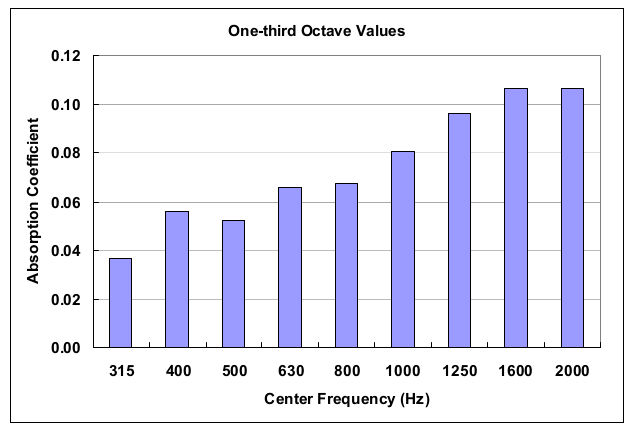
\includegraphics[width=0.7\textwidth]{fig/chap4/impedance/absorption_spectrum.png}
	\caption{Absorption coefficient in one-third octave bands \cite{Seybert2008MeasurementOP}}
	\label{fig:ground_absorption}
\end{figure}

\begin{table}[H]
	\caption{Estimated absorption coefficient from fig. \ref{fig:ground_absorption}, the values for frequency lower than 315 Hz are chosen arbitrary}
	\begin{tabular}{c|ccccccc}
		Freq (Hz)           & 100  & 125  & 160  & 200  & 250  & 315  & 400 \\ \hline
		$\alpha$ & 0.02 & 0.02 & 0.02 & 0.02 & 0.02 & 0.035 & 0.055
	\end{tabular}
	\newline
	\vspace*{10pt}
	\newline
	\begin{tabular}{c|ccccccc}
		Freq (Hz)  &  500  & 630  & 800  & 1000 & 1250 & 1600 & 2000 \\ \hline
		$\alpha$ & 0.05 & 0.065 & 0.065 & 0.08 & 0.095 & 0.105 & 0.105
	\end{tabular}
\end{table}

\begin{equation}
	\alpha = 1 - |r^2|
\end{equation}

\begin{equation}
	r = \frac{Z_s - Z_0}{Z_s + Z_0} = \frac{\frac{Z_s}{Z_0} - 1}{\frac{Z_s}{Z_0} + 1}
\end{equation}

\begin{equation}
	\tilde{Z_s} = \frac{Z_s}{Z_0} = \tilde{R} + j\tilde{X}
\end{equation}



\begin{equation}
	\begin{cases}
		\frac{4\tilde{R_s}}{\tilde{R_s}^2+\tilde{X_s}^2 + 2\tilde{R_s} + 1} = \alpha\\
		\arctan{\frac{\tilde{X_s}}{\tilde{R_s}}} = \varphi
	\end{cases}	
	\label{eq:impedance}
\end{equation}


\begin{figure}[H]
	\centering
	\begin{subfigure}[b]{0.8\textwidth}
		\centering
		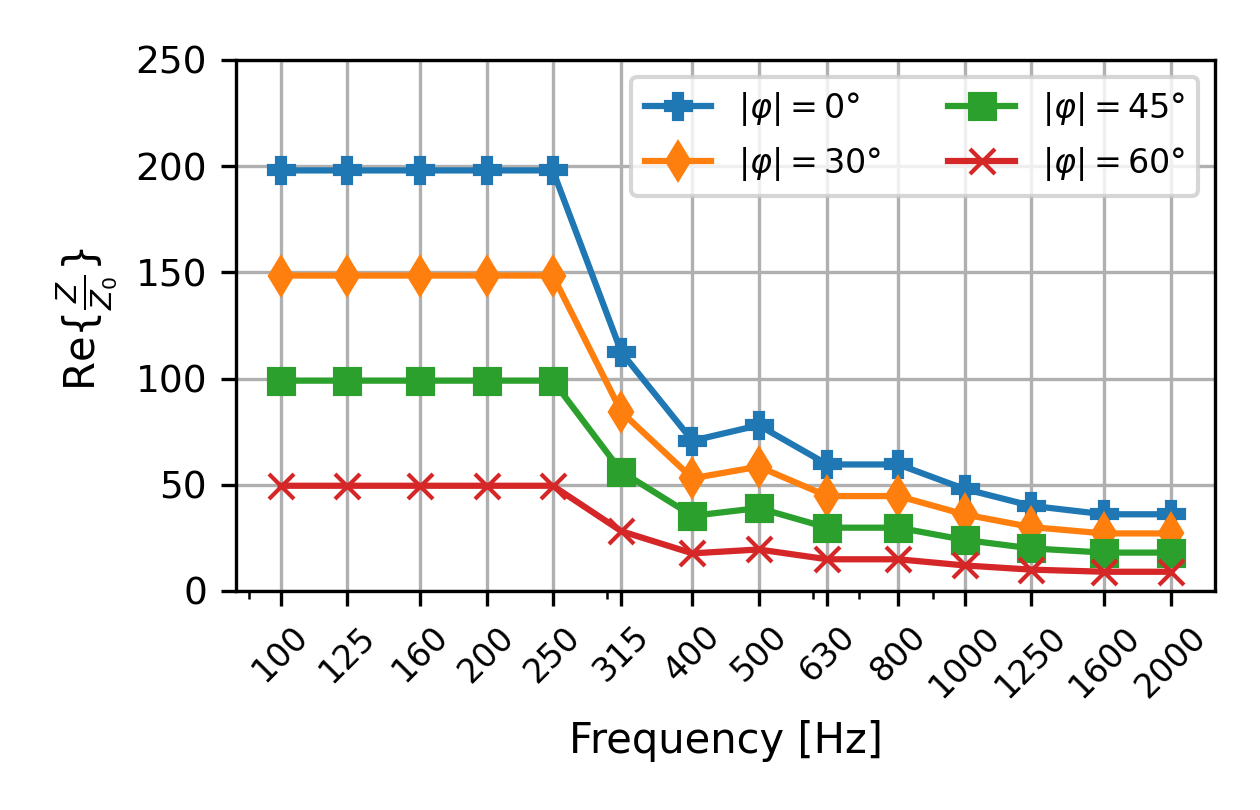
\includegraphics{fig/chap4/impedance/impedance_real.png}
	\end{subfigure}
	\begin{subfigure}[b]{0.8\textwidth}
		\centering
		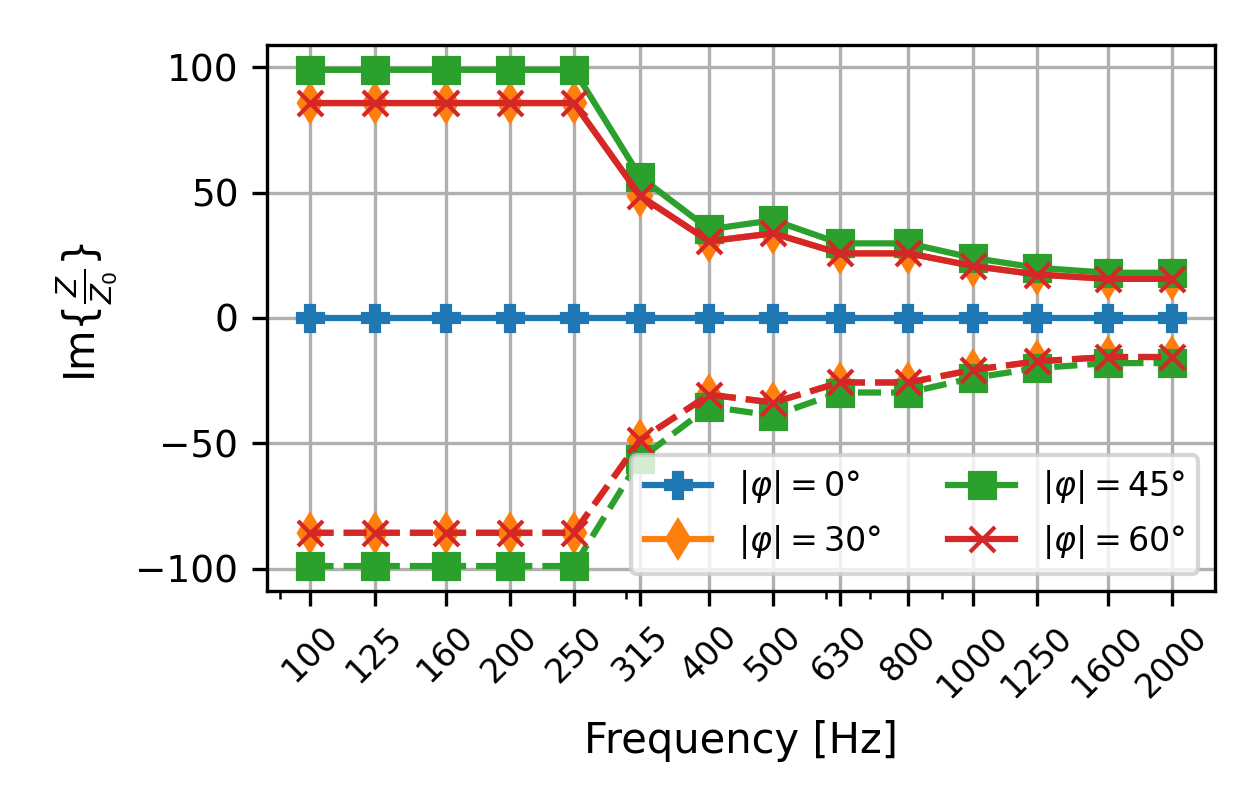
\includegraphics{fig/chap4/impedance/impedance_imag.png}
	\end{subfigure}
	\caption{Input impedance in one-third octave bands}
\end{figure}


\subsection{Variation of frequency steps per 1/3-octave band}

\chapter{Results and Discussions}
\label{chap:results}

In the following, the results obtained from the finite element simulation using different setups are discussed and compared to the outer pressure field measurement.

\section{Comparison of simulation and measurement results}



\begin{figure}[H]
	% Einheiten: "quantity" in "unit", nicht [unit] !
	\centering
	\begin{subfigure}[b]{0.49\textwidth}
		\centering
		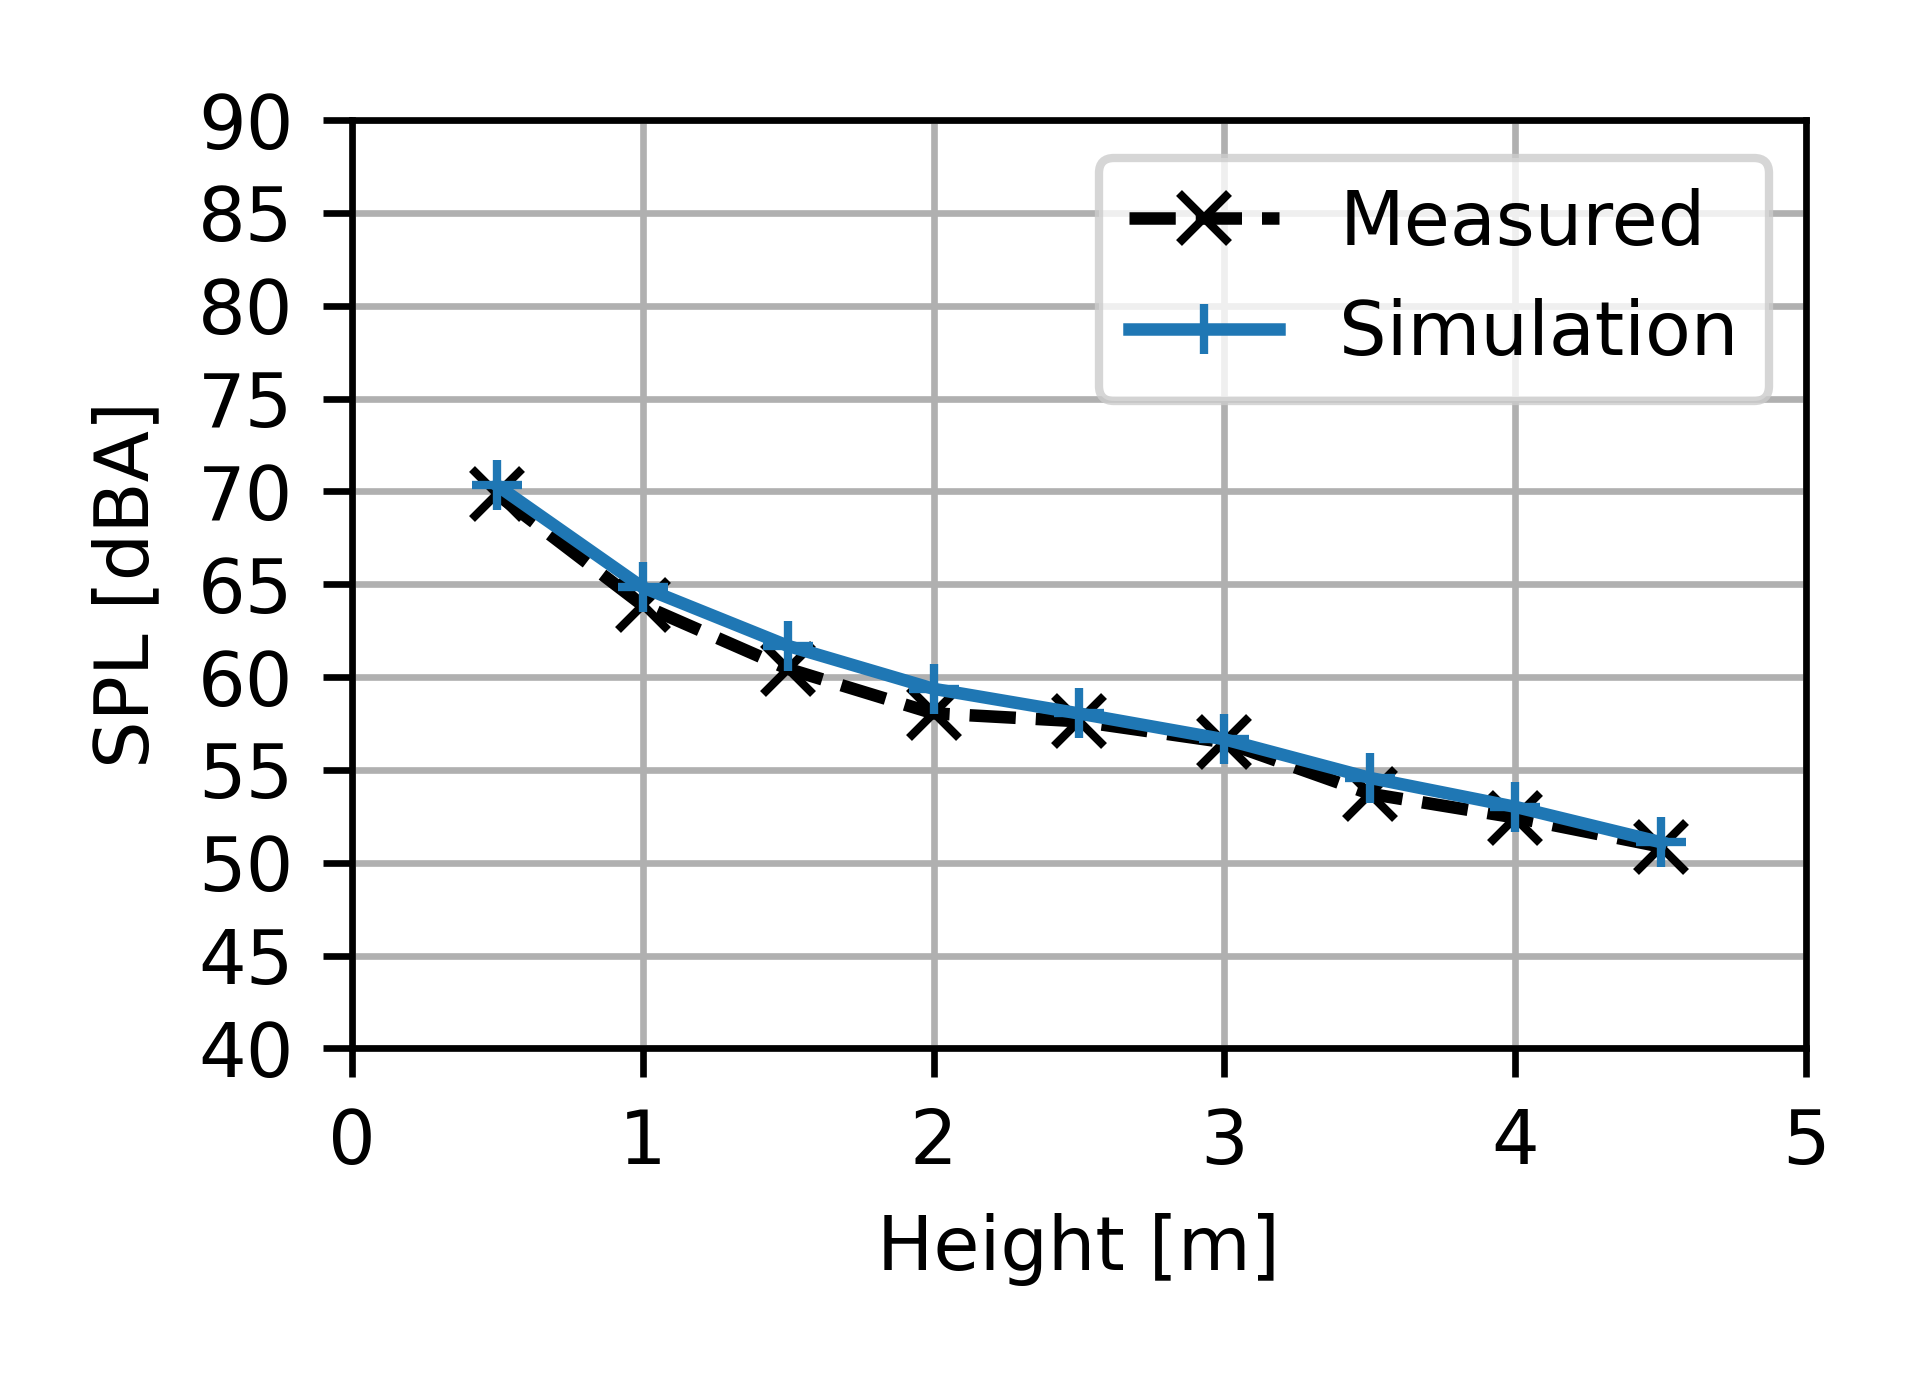
\includegraphics{fig/chap5/initial_model/third_octave_over_height/125_Hz.png}
		\caption{125 Hz}
	\end{subfigure}
	\hfill
	\begin{subfigure}[b]{0.49\textwidth}
		\centering
		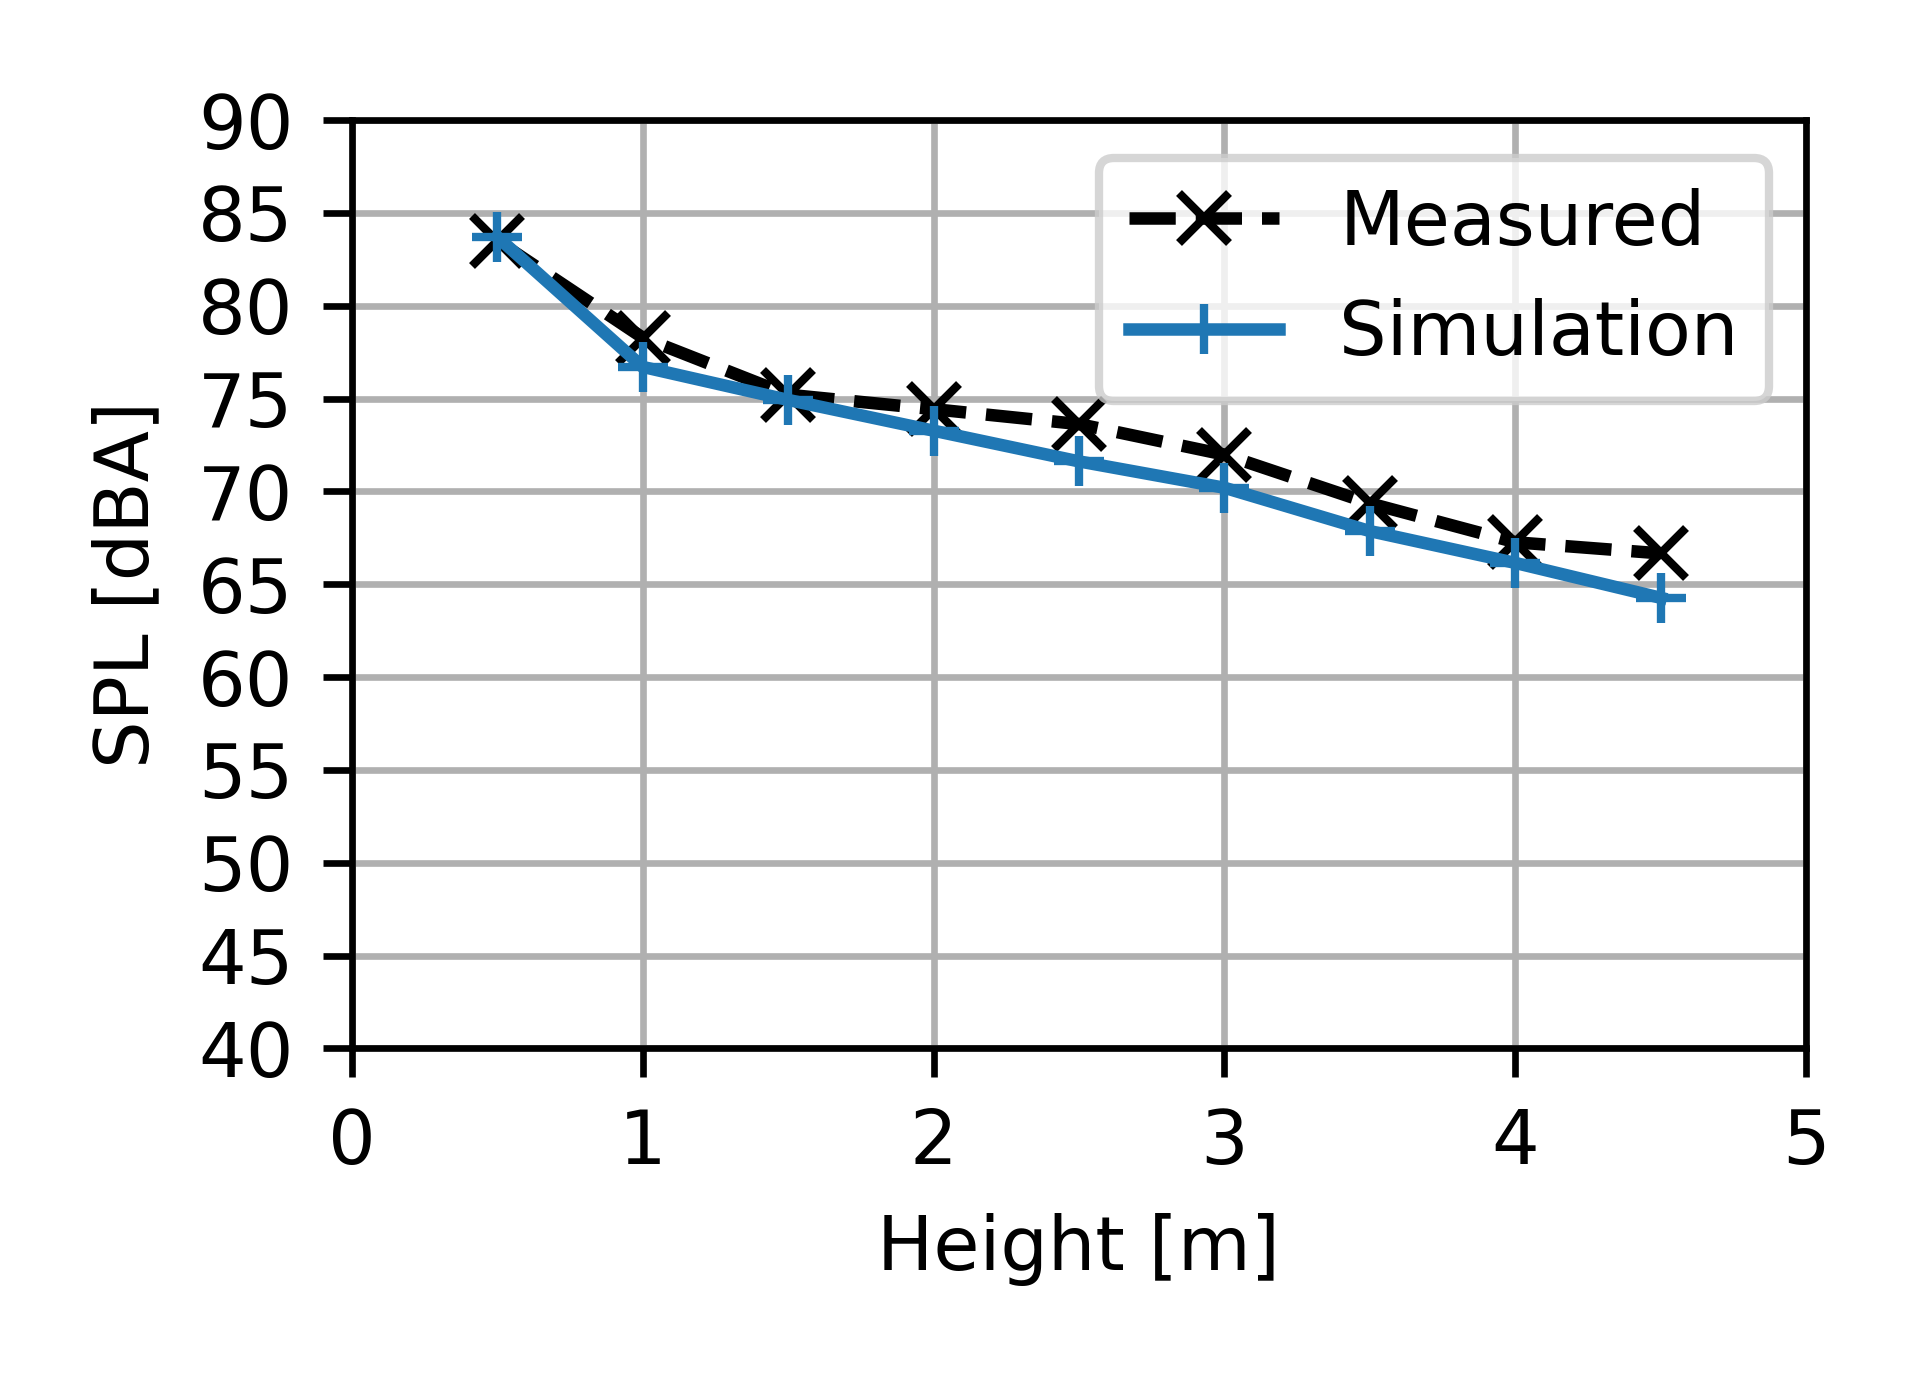
\includegraphics{fig/chap5/initial_model/third_octave_over_height/400_Hz.png}
		\caption{400 Hz}
	\end{subfigure}
	\\
	\begin{subfigure}[b]{0.49\textwidth}
		\centering
		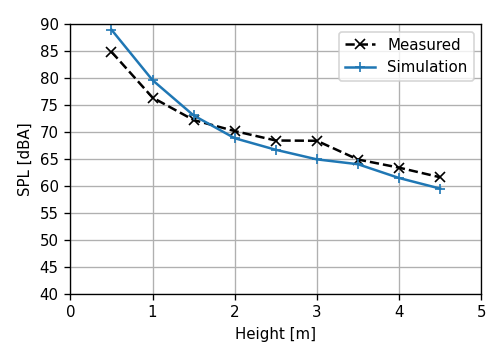
\includegraphics{fig/chap5/initial_model/third_octave_over_height/1250_Hz.png}
		\caption{1250 Hz}
	\end{subfigure}
	\hfill
	\begin{subfigure}[b]{0.49\textwidth}
		\centering
		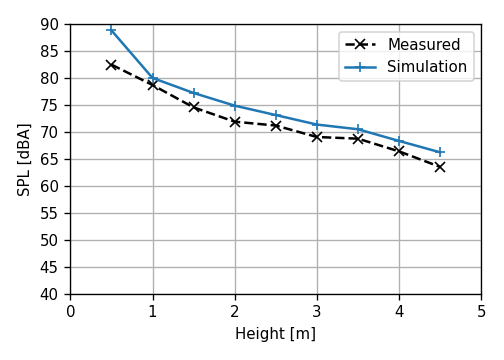
\includegraphics{fig/chap5/initial_model/third_octave_over_height/2000_Hz.png}
		\caption{2000 Hz}
	\end{subfigure}
	\caption{Sound distribution at measurement position a, comparison between predictions obtained from the initial finite element model with the measurements. A-weighted SPL in one-third octave bands, dBA ref 20 $\mu$Pa.}
	\label{fig:third_octave_over_height}
\end{figure}

\noindent In fig. \ref{fig:third_octave_over_height}, the A-weighted sound pressure levels at measurement position a (10 cm away from vehicle) along the car body height in example one-third octave bands are shown. The simulation result is compared with the measurement value at each microphone position. One can see that for 125 Hz and 400 Hz, the simulation fits the measured curves very well. A greater difference between the simulation and the measurement occurs for 1250 Hz and 2000 Hz, but the measured shape is still well approximated for both frequency bands. Other bands show similar results, and the model captures the measured sound pressure level trends well.

\begin{figure}[H]
	\centering
	\begin{subfigure}[b]{0.49\textwidth}
		\centering
		\includegraphics{fig/chap5/initial_model/overall_SPL/all_pos.png}
		%\caption{2000 Hz}
	\end{subfigure}
	\hfill
	\begin{subfigure}[b]{0.49\textwidth}
		\centering
		\includegraphics{fig/chap5/initial_model/overall_SPL/deviation.png}
		%\caption{2000 Hz}
	\end{subfigure}
	\caption{Comparison of overall SPL in dBA ref 20 $\mu$Pa. Left: overall SPL as a function of height at various measurement positions (dashed curves: measurement; solid curves: simulation) Right: deviation between simulation and measurement results.}
	\label{fig:overall_SPL}
\end{figure}

\noindent The overall sound pressure level is a simple and direct parameter to quantify the sound level. For comparison, the A-weighted sound pressure levels of each one-third octave band from 100 Hz to 2000 Hz are added up. Fig. \ref{fig:overall_SPL} shows the overall A-weighted sound pressure level at three different measurement positions and the deviation between the simulated and measured results. As can be seen from the results, the predictions of overall sound pressure levels at the three distances from the car body agree well with the measurement. For all three measurement positions, the maximum deviation between the simulation and measurement results occurs at 0.5 m, which is at the height of the bogie. At these locations, the simulation results are 1.5 dB to 3 dB higher than the measured values. In general, the approximation is getting better with increasing height. In the area above 2m, the difference between the simulation and the measurement in terms of overall sound pressure is within 1 dB.

\begin{figure}[H]
	\centering
	\begin{subfigure}[b]{0.49\textwidth}
		\centering
		\includegraphics{fig/chap5/initial_model/freq_spectrum/pos_10cm_0pt5m.png}
		\caption{0.5 m}
	\end{subfigure}
	\hfill
	\begin{subfigure}[b]{0.49\textwidth}
		\centering
		\includegraphics{fig/chap5/initial_model/freq_spectrum/pos_10cm_1pt5m.png}
		\caption{1.5 m}
	\end{subfigure}
\end{figure}
\begin{figure}[H] \ContinuedFloat
	\begin{subfigure}[b]{0.49\textwidth}
		\centering
		\includegraphics{fig/chap5/initial_model/freq_spectrum/pos_10cm_2pt5m.png}
		\caption{2.5 m}
	\end{subfigure}
	\hfill
	\begin{subfigure}[b]{0.49\textwidth}
		\centering
		\includegraphics{fig/chap5/initial_model/freq_spectrum/pos_10cm_4pt5m.png}
		\caption{4.5 m}
	\end{subfigure}
	\caption{1/3-octave spectra of the A-weighted SPL for simulation and measurement data at selected microphone positions.}
	\label{fig:freq_spectrum}
\end{figure}

\noindent\Cref{fig:freq_spectrum} shows the spectra of the A-weighted sound pressure level in one-third octave bands. The SPL spectra are evaluated at the measurement position a (10 cm away from the vehicle) at different microphone locations. As can be seen from the results, the simulation fits the measured spectra well, the measured trend is well captured. Again, a larger deviation between the simulated and measured results occurs at 0.5 m above ground and the approximation is getting better with increasing height.

In order to have an idea of the model accuracy of each 1/3-octave band, the mean relative error between the simulation result and the measurement for each 1/3-octave band over all 27 microphone positions will be computed. To compute the mean relative error, the sound pressure level is first converted back to linear scaling by
\begin{equation}
	p(\text{Pa}) = p_0 \cdot 10^{\frac{\text{SPL}}{20}} = 2\cdot10^{-5}\,\text{Pa} \cdot 10^{\frac{\text{SPL}}{20}}\text{.}
\end{equation}
The mean relative error (MRE) is then defined as
\begin{equation}
	\text{MRE}(p_{\text{measured}}, p_{\text{simulation}}) = \frac{1}{N} \sum_{i=0}^{N - 1} \frac{|p_{\text{simulation,}i} - p_{\text{measured,}i}|}{|p_{\text{measured,}i}|}\,.
\end{equation}
The mean relative error can also be converted to decibels using the relation
\begin{equation}
	\text{MRE(dB)} = 20\cdot\log_{10}(1 + \text{MRE})\,.
\end{equation}

\begin{figure}[H]
	\centering
	\includegraphics{fig/chap5/initial_model/freq_spectrum/average_gap.png}
	\caption{Mean relative error between simulation result and measurement for each 1/3-octave band over all 27 microphone positions}
	\label{fig:gap_freq_spectrum}
\end{figure}

\begin{table}[H]
	\caption{Mean relative error of 1/3-octave frequency spectrum over all microphone positions}
	\begin{tabular}{c|cccccccccccccc}
		Freq (Hz)           & 100  & 125  & 160  & 200  & 250  & 315  & 400  & 500  & 630  & 800  & 1000 & 1250 & 1600 & 2000 \\ \hline
		MRE (dB) & 2.34 & 0.55 & 3.06 & 3.51 & 1.34 & 1.82 & 1.06 & 1.67 & 1.53 & 1.97 & 3.36 & 2.15 & 2.45 & 2.65
	\end{tabular}
	\label{tab:MRE_spectra}
\end{table}

\noindent The mean relative error in terms of the sound pressure levels over all 27 microphone positions at each frequency band between the predictions and the measurements are shown in fig. \ref{fig:gap_freq_spectrum} and in tab. \ref{tab:MRE_spectra}. As can be seen from the results, the best approximation occurs for 125 Hz band which has the smallest mean relative error among all 1/3 octave bands. Three frequency bands (160, 200 and 1000 Hz) have an error over 3 dB, and the maximum error is limited by 3.5 dB. Good approximation has also been shown for the frequency band from 250 to 800 Hz, for which the mean relative errors are within 2 dB. The average gap per frequency band is obtained by averaging the mean relative error spectrum over all 14 one-third octave bands. Following the same idea, the mean relative error in terms of overall sound pressure levels will also be used as a metric for model accuracy.

The average gap per frequency band and the mean relative error of overall sound pressure levels over all microphone positions are shown in \cref{tab:average_gap}.
\begin{table}[H]
	\centering
	\caption{Average gap per frequency band and mean relative error of overall SPL of initial model}
	\begin{tabular}{c|c}
		Average gap per  frequency band (dB) & Mean relative error of overall SPL (dB) \\ \hline
		%$2.14\pm1$  & $0.73\pm0.86$
		2.14 & 0.73
	\end{tabular}
	\label{tab:average_gap}
\end{table}
\noindent The average difference per frequency band is 2.14 dB and the mean relative error of the overall sound pressure level is 0.73 dB. From these results it can be concluded that the finite element model is able to predict the sound transmission from the train underfloor adequately.


\section{Effect of geometric variation}

In this section, the results obtained by the variation analysis of underfloor geometry are shown. The geometrical models are illustrated and explained in section \ref{section:variation_geometry}.

\begin{figure}[H]
	\centering
	\begin{subfigure}[b]{0.49\textwidth}
		\centering
		\includegraphics{fig/chap5/geometry_variation/third_octave_over_height/100_Hz.png}
		\caption{100 Hz}
	\end{subfigure}
	\hfill
	\begin{subfigure}[b]{0.49\textwidth}
		\centering
		\includegraphics{fig/chap5/geometry_variation/third_octave_over_height/250_Hz.png}
		\caption{250 Hz}
	\end{subfigure}
	\\
	\begin{subfigure}[b]{0.49\textwidth}
		\centering
		\includegraphics{fig/chap5/geometry_variation/third_octave_over_height/500_Hz.png}
		\caption{500 Hz}
	\end{subfigure}
	\hfill
	\begin{subfigure}[b]{0.49\textwidth}
		\centering
		\includegraphics{fig/chap5/geometry_variation/third_octave_over_height/1000_Hz.png}
		\caption{1000 Hz}
	\end{subfigure}
	\caption{Sound distribution at measurement position a, comparison between different geometrical models with the measurements. A-weighted SPL in one-third octave bands, dBA ref 20 $\mu$Pa.}
	\label{fig:third_octave_over_height_geometry_variation}
\end{figure}

\noindent\Cref{fig:third_octave_over_height_geometry_variation} shows the A-weighted sound pressure level at measurement position a (10 cm away from vehicle) for different geometry variations in example one third octave bands. As can be seen from the results, at the lowest frequency band (100 Hz), there is almost no difference between the different models. This may due to the much larger wavelength (about 3.43 meter for 100 Hz) than the physical dimension of the geometry. At this frequency, all four models overestimates the sound pressure level by about 3 dB but are still able to capture the measured curve shape well. Large deviation between the models is found at 250 Hz, where the model without underfloor components shows an huge underestimation of the result and the model with additional structures tends to overestimate while the initial model and the model without air suspension are showing very good agreement with the measurement data. For 500 Hz and 1000 Hz, the model with additional structures and the model without air suspension are closest to the measurement data, respectively. In general, all models show similar shape as the measurement curves, the differences in terms of sound pressure level between the four models are within 10 dB. The same results are also observed for other frequency bands.

\begin{figure}[H]
	\centering
	\begin{subfigure}[b]{\textwidth}
		\centering
		\includegraphics{fig/chap5/geometry_variation/overall_SPL/pos_a.png}
		\hfill
		\includegraphics{fig/chap5/geometry_variation/overall_SPL/pos_a_deviation.png}
		\caption{10 cm away from car body}
	\end{subfigure}
	\\
	\begin{subfigure}[b]{\textwidth}
		\centering
		\includegraphics{fig/chap5/geometry_variation/overall_SPL/pos_f.png}
		\hfill
		\includegraphics{fig/chap5/geometry_variation/overall_SPL/pos_f_deviation.png}
		\caption{50 cm away from car body}
	\end{subfigure}
	\caption{Comparison of overall A-weighted SPL for different geometrical models. Left: overall SPL as a function of height at various measurement positions. Right: difference between simulation and measurement results.}
	\label{fig:overall_SPL_geometry}
\end{figure}

\noindent\Cref{fig:overall_SPL_geometry} shows the distribution of  A-weighted overall sound pressure levels at different distances from the car body for different geometrical models. The difference between the simulation and the measurement results are plotted in the right figures. As can be seen from the figures, all four models show similar results in the lower area (up to 2 m height), the deviation between the models starts to grow with increasing height. Comparing the initial model and the model without air suspension, the model without air suspension shows a greater overestimation of the overall SPL than the initial model, at the height of bogie (0.5 m). Up from 1.5 m height, both models show very good agreement with the measurement results and there is almost no difference between both models. One can also see, without including any underfloor components into the model, the overall SPL is overestimated at each measurement location due to a lack of attenuation of the acoustic wave by the underfloor components. The difference between the initial model and the model without underfloor components is about 1 to 1.5 dB depending on the measurement locations. The model with additional underfloor structures shows a similar result as the initial model at 0.5 m height, but in the higher region (up from 1.5 m), the result converges to that of the model without underfloor components.

\begin{figure}[H]
	\centering
	\includegraphics[width=0.7\linewidth]{fig/chap5/geometry_variation/freq_spectrum/average_gap.png}
	\caption{Mean relative error of 1/3-octave frequency}
	\label{fig:gap_freq_spectrum_geometry}
\end{figure}

\noindent\Cref{fig:gap_freq_spectrum_geometry} shows the mean relative error spectra for the four geometrical models over all 27 microphone locations, the spectrum of the initial model has also been shown in \cref{fig:gap_freq_spectrum}. As can be seen from the figure, all three geometry variations show greater maximum error than the initial model. For a large part of the frequency bands, the model without underfloor components has the greatest deviation among the models. At frequency band 100, 315, 400, 630 and 2000 Hz, the difference in terms of the mean relative error among the models is small and limited by 1 dB. The initial model and the model without air suspension share similar results, but at frequency band 800, 1000, 1600 and 2000 Hz, the latter model shows better approximation than the former.

\begin{table}[H]
	\centering
	\caption{Average gap per frequency band and mean relative error in overall SPL for different geometry variations}
	\label{tab:geometry_variation_MRE}
	\begin{tabular}{c|c|c}
		Geometry name              & Average gap per frequency band (dB) & MRE overall SPL (dB) \\ \hline
		No underfloor components   & $3.12$                       & $1.78$        \\
		No air suspension          & $2.21$                       & $0.85$        \\
		Initial model              & $2.34$                       & $0.73$        \\
		With additional structures & $2.57$                       & $1.30$       
	\end{tabular}
\end{table}

\noindent In order to quantify the difference between the geometry variations, the average gap per frequency band and the mean relative error in terms of overall SPL are computed and shown in \cref{tab:geometry_variation_MRE}. The table is ordered by the complexity of the modeled geometry. As can be seen from results, the simplest model, namely the model without any underfloor components, shows the greatest average gap per frequency band as well as the largest mean relative error in terms of the overall sound pressure level. Both errors are reduced by almost 1 dB by including the most essential underfloor components (bogie and wheel) into the model. Taking the air suspension into account leads to a better approximation for the overall SPL, but a slightly increased average gap per frequency band, which may due to the sound hard assumption of the air suspension surface. Surprisingly, the model with additional structures shows a greater deviation in both metrics compared to the initial model. It was expected that including more underfloor details will also lead to a better approximation of the measurement. It can be concluded from the results shown in this section that the number of modeled underfloor components do affect the prediction accuracy of the finite element model. To achieve better approximation of the measurement data, at least the bogie and the wheel should be taken into the geometrical model. Without modeling the underfloor components, the predicted overall SPL is about 1 dB higher compared to the prediction using model with underfloor components.

\section{Effect of ground absorption}

In this section, the simulation results obtained by the variation analysis of the surface impedance are shown. Noticed that all variation models have the same normal incident absorption coefficient and only differ in their impedance phase angle. Since the absorption data used for the simulation is fictive, the results are not compared to the validation measurement but to the initial model with fully reflective ground.

\begin{figure}[H]
	\centering
	\begin{subfigure}[b]{\textwidth}
		\centering
		\includegraphics{fig/chap5/impedance/third_octave/SPL_100_Hz.png}
		\hfill
		\includegraphics{fig/chap5/impedance/third_octave/deviation_100_Hz.png}
		\caption{100 Hz}
	\end{subfigure}
	\\
	\begin{subfigure}[b]{\textwidth}
		\centering
		\includegraphics{fig/chap5/impedance/third_octave/SPL_1000_Hz.png}
		\hfill
		\includegraphics{fig/chap5/impedance/third_octave/deviation_1000_Hz.png}
		\caption{1000 Hz}
	\end{subfigure}
\end{figure}
\begin{figure}[H]\ContinuedFloat
	\begin{subfigure}[b]{\textwidth}
		\centering
		\includegraphics{fig/chap5/impedance/third_octave/SPL_2000_Hz.png}
		\hfill
		\includegraphics{fig/chap5/impedance/third_octave/deviation_2000_Hz.png}
		\caption{2000 Hz}
	\end{subfigure}

	\caption{Sound distribution at measurement position a, comparison between the model with full reflective ground and the models with different impedance phase angles. Solid curves: positive phase angle. Dashed curves: negative phase angle.}
	\label{fig:third_octave_over_height_impedance}
\end{figure}

\noindent \Cref{fig:third_octave_over_height_impedance} shows the A-weighted sound pressure level at measurement position a (10 cm away from vehicle) along the car body height for models with different impedance phase angles in example one third octave bands. The simulation results are compared to the result obtained by the model without ground absorption (initial model) and the difference is also shown in the figures. The solid lines represent the results with positive phase angle and the dashed lines those of the negative phase angle, respectively. As can be seen from the results, for 100 Hz, there is almost no noticeable difference between the absorption models and the initial model due to the small absorption coefficient (2 percent) in the low frequency range. For frequencies with higher absorption coefficient, a decrease in sound pressure level due to absorption becomes more visible. One can see that the degree of absorption within a frequency band strongly depends on the phase angle of the complex surface impedance. In general, the greater the impedance angle the stronger the absorption. An exception exists for the model with zero phase angle, which contains only real part, its curve lays between those of positive and negative 45-degree angle. Also, it can be seen that the absorptance also depends on the sign of the impedance phase angle, the negative angle (dashed line) has a slightly stronger absorptance than its complex conjugate (solid line), and the difference between the complex conjugate pair grows with the absolute phase angle. For phase angles with same sign, they share the same curve shape and only differ in their absolute values.

\begin{figure}[H]
	\centering
	\begin{subfigure}[b]{\textwidth}
		\centering
		\includegraphics{fig/chap5/impedance/overall_SPL/overall_SPL_pos_a.png}
		\includegraphics{fig/chap5/impedance/overall_SPL/deviation_pos_a.png}
		\caption{10 cm away from carbody}
	\end{subfigure}
\end{figure}
\begin{figure}[H]\ContinuedFloat
	\begin{subfigure}[b]{\textwidth}
		\centering
		\includegraphics{fig/chap5/impedance/overall_SPL/overall_SPL_pos_f.png}
		\includegraphics{fig/chap5/impedance/overall_SPL/deviation_pos_f.png}
		\caption{50 cm away from carbody}
	\end{subfigure}
	\begin{subfigure}[b]{\textwidth}
		\centering
		\includegraphics{fig/chap5/impedance/overall_SPL/overall_SPL_pos_g.png}
		\includegraphics{fig/chap5/impedance/overall_SPL/deviation_pos_g.png}
		\caption{100 cm away from carbody}
	\end{subfigure}
	
	\caption{Comparison of overall A-weighted sound pressure level between difference impedance phase angles.Solid curves: positive phase angle. Dashed curves: negative phase angle.}
	\label{fig:overall_SPL_impedance}
\end{figure}

\noindent Very similar results are also observed in the overall sound pressure level distribution, which is shown in fig. \ref{fig:overall_SPL_impedance}. Again, the impedance phase angle dependency of absorption can be seen from the results. That is to say, the greater the phase angle, the greater the deviation to the full reflective model and hence, the higher the absorption. The greatest difference in terms of overall sound pressure level among the investigated phase angles is about 1 dB. Furthermore, for a complex conjugate pair with the same absolute impedance phase angle, that with negative phase angle (dashed line) shows higher absorptance than the positive one (solid line). And the deviation among the conjugate pair grows with the absolute phase angle. In case of zero phase angle, whose surface impedance contains only real part, its result lays between those of the 45-degree complex conjugate pair.

\begin{figure}[H]
	\centering
	\includegraphics[width=0.7\linewidth]{fig/chap5/impedance/freq_spectrum/average_gap.png}
	\caption{Mean relative deviation in terms of sound pressure level compared to full reflective model in 1/3-octave band. Solid curves: positive phase angle. Dashed curves: negative phase angle.}
	\label{fig:gap_freq_spectrum_impedance}
\end{figure}

\noindent\Cref{fig:gap_freq_spectrum_impedance} shows the mean relative deviation spectra in terms of sound pressure level for different impedance phase angles compared to the initial model with fully reflective ground. As can be seen from the results, in low frequency region between 100 and 315 Hz, where the absorption coefficient is small (2 to 3 percent), the difference in results between the different phase angles is also small. With growing absorption coefficient, the deviation between the phase angles gets larger. The largest difference occurs in the high frequency region, in this case between 1000 Hz and 2000 Hz, where the deviation is about 1.5 dB.

\begin{table}[H]
	\centering
	\caption{Mean deviation in overall SPL for different impedance phase angles}
	\label{tab:mean_devaition_impedance}
	\begin{tabular}{cc}
		\toprule
		$\text{arg}(\tilde{R_s} + j\tilde{X_s})$ (°) & Average deviation in overall SPL (dB) \\
		\midrule
		0                         & 0.72                                      \\
		30/-30                    & 0.46/0.55                                 \\
		45/-45                    & 0.66/0.78                                 \\
		60/-60                    & 1.15/1.34                                 \\
		\bottomrule
	\end{tabular}
\end{table}

\noindent The average deviation in terms of overall sound pressure level compared to the full reflective model can be found in tab. \ref{tab:mean_devaition_impedance}. A larger deviation to full reflective model means a larger absorption of the sound pressure. One can see that the difference between the smallest and the largest absorption degree is about 1 dB. And the absorptance of 0-degree angle is the median of the result set.

From the results shown in this section it can be concluded that for a given normal incident absorption coefficient spectrum, the actual absorption of the acoustic wave depends on the phase angle of the complex surface impedance. For the case that only absorption data is available, it can be assumed that the surface impedance contains only real part. In order to obtain a more accurate simulation result, not only the absorption spectrum of the material should be provided, but also the full impedance characteristic of the ground surface. This information can be obtained by for example an in-situ measurement of surface impedance using impedance tube method as described in \cite{hald_situ_2019, wolkesson_2013}.

\section{Effect of varing frequency steps per 1/3-octave band}

In this section, the simulation results obtained by variation analysis using different intermediate frequency steps in single 1/3-octave band are shown.

\begin{figure}[H]
	\centering
	\begin{subfigure}[b]{0.49\textwidth}
		\centering
		\includegraphics{fig/chap5/freq_steps/third_octave_over_height/100_Hz.png}
		\caption{100 Hz}
	\end{subfigure}
	\hfill
	\begin{subfigure}[b]{0.49\textwidth}
		\centering
		\includegraphics{fig/chap5/freq_steps/third_octave_over_height/315_Hz.png}
		\caption{315 Hz}
	\end{subfigure}
	\\
	\begin{subfigure}[b]{0.49\textwidth}
		\centering
		\includegraphics{fig/chap5/freq_steps/third_octave_over_height/630_Hz.png}
		\caption{630 Hz}
	\end{subfigure}
	\hfill
	\begin{subfigure}[b]{0.49\textwidth}
		\centering
		\includegraphics{fig/chap5/freq_steps/third_octave_over_height/2000_Hz.png}
		\caption{2000 Hz}
		\label{fig:curve_sink}
	\end{subfigure}
	
	\caption{A-weighted sound pressure level in example one-third octave bands at measurement position a. For different intermediate steps per one-third octave band.}
	
	\label{fig:third_octave_over_height_freq_steps}
\end{figure}

\noindent\Cref{fig:third_octave_over_height_freq_steps} shows the sound distribution at measurement position a (10 cm away from vehicle) along the height direction for different frequency resolution of one-third octave band. As can be seen from the results, for 100 Hz, there is almost no noticeable difference in results between the different frequency steps due to its narrow bandwidth of about 23 Hz. With increasing one-third octave band frequency and hence an increasing bandwidth, using one single intermediate frequency step to resolve the one-third octave band is not enough. At 315 Hz, the predicted sound pressure level using only single step is about 5 dB lower than the results obtained with more frequency steps. In 630 and 2000 Hz band, when using only the center frequency to represent the one third octave band, destructive interference effect in the sound distribution can be observed. The sink in the sound pressure curve is smoothed out once more intermediate frequency steps are used to compute the one third octave band result. Except for the single step, results obtained by using 3, 5 and 9 intermediate steps are in the same range and agree well with the measurement.

\begin{figure}[H]
	\centering
	\begin{subfigure}[b]{0.3\textwidth}
		\centering
		\includegraphics[width=\linewidth]{fig/chap5/freq_steps/field_result_1781Hz.png}
		\caption{1781 Hz}
	\end{subfigure}
	\hfill
	\begin{subfigure}[b]{0.3\textwidth}
		\centering
		\includegraphics[width=\linewidth]{fig/chap5/freq_steps/field_result_2000Hz.png}
		\caption{2000 Hz}
		\label{fig:field_2000Hz}
	\end{subfigure}
	\hfill
	\begin{subfigure}[b]{0.3\textwidth}
		\centering
		\includegraphics[width=\linewidth]{fig/chap5/freq_steps/field_result_2245Hz.png}
		\caption{2245 Hz}
	\end{subfigure}
	\caption{Pressure field of three frequencies in 2000 Hz one third octave band. The green line marks the evaluation position of the sound pressure level.}
	\label{fig:pressure_field_solution}
\end{figure}

\noindent\Cref{fig:pressure_field_solution} shows the pressure field of three frequencies within the 2000 Hz one third octave band. The frequencies are corresponding to the lower band limit, the center frequency and the upper band limit of the one third octave band, respectively. The sink in the sound pressure level curve using only single step as shown in fig. \ref{fig:curve_sink} is due to the destructive interference of the acoustic wave, which can be seen in fig. \ref{fig:field_2000Hz}. The blue area at the middle of the car body wall indicates a sink in the acoustic pressure. If more intermediate frequency steps are used, the sink in the sound pressure level curve will get averaged out since no destructive interference occurs at the same location in the pressure field of other frequencies.

\begin{figure}[H]
	\begin{subfigure}[b]{\textwidth}
		\centering
		\includegraphics[width=0.49\textwidth]{fig/chap5/freq_steps/overall_SPL/pos_a.png}
		\includegraphics[width=0.49\textwidth]{fig/chap5/freq_steps/overall_SPL/pos_a_deviation.png}
		\caption{10 cm away from car body}
	\end{subfigure}
\end{figure}
\begin{figure}[H]\ContinuedFloat
	\begin{subfigure}[b]{\textwidth}
		\centering
		\includegraphics[width=0.49\textwidth]{fig/chap5/freq_steps/overall_SPL/pos_f.png}
		\includegraphics[width=0.49\textwidth]{fig/chap5/freq_steps/overall_SPL/pos_f_deviation.png}
		\caption{50 cm away from car body}
	\end{subfigure}
	\caption{Comparison of overall A-weighted sound pressure level using different intermediate frequency steps per one third octave}
	\label{fig:overall_SPL_freq_steps}
\end{figure}

\noindent\Cref{fig:overall_SPL_freq_steps} shows the overall A-weighted sound pressure level distribution obtained by using different intermediate frequency steps compared to the measurement. The overall SPL curves are shown in the figures left and the deviations to the measurement are shown in the figures right, respectively. As can be seen from the figures, at most of the microphone locations, the simulation using 9 frequency steps per one third octave band shows the closest fit to the measurement while the results obtained by using 3 or 5 intermediate steps are also in the same range, but with a slightly greater deviation. When using only one single frequency step, a noticeable difference to the measured SPL curve at 2 to 4 m height can be observed. This is also the range of height where for several one third octave band center frequencies the sinks in sound pressure level curves are located, as previously shown in fig. \ref{fig:third_octave_over_height}.

\begin{table}[H]
	\caption{Mean relative error in overall SPL and total computation time using different intermediate frequency steps per one third octave band}
	\label{tab:freq_steps_MRE}
	\begin{tabularx}{\columnwidth}{|X|c|c|}
	\hline
	\textbf{Intermediate step per one third octave band} & \textbf{MRE in overall SPL {[}dB{]}} & \textbf{Total computation time {[}hour{]}} \\ \hline
	\hspace{65pt} 1                                                    & 1.10                                 & 4.5                                        \\ \hline
	\hspace{65pt} 3                                                    & 0.82                                 & 10                                         \\ \hline
	\hspace{65pt} 5                                                    & 0.76                                 & 15                                         \\ \hline
	\hspace{65pt} 9                                                    & 0.73                                 & 27                                         \\ \hline
	\end{tabularx}
\end{table}

\noindent\Cref{tab:freq_steps_MRE} shows the mean relative error in terms of the overall A-weight sound pressure level to the measurement obtained by using different intermediate frequency steps per one third octave band. Further, the total computation time for all 14 one third octave bands covering 100 to 2000 Hz is also shown in the same table. As expected, the more intermediate steps per one third octave band are used, the better the approximation to the measured results. On the other hand, it can be seen that the convergence rate of the mean relative error is getting slower with increasing intermediate steps, which means upon a certain degree of frequency resolution, better approximation can not be achieved by simply using more intermediate frequency steps per one third octave band. Another important aspect of choosing the proper number of intermediate frequency steps is the total computation time of the simulation, which increases linearly with the number of frequency steps. For our finite element model, choosing 5 intermediate steps per one third octave band would be a good compromise between accuracy and computational effort, since it has a similar mean relative error in terms of overall sound pressure level as the initial setup with 9 intermediate steps but saves up almost 50 per cent of the computation time.

From the results shown in this section it can be concluded that the number of intermediate frequency steps used per one third octave band do affect the prediction accuracy of the finite element model. At low frequency range, using one single frequency step to resolve the one third octave band is sufficient while with increasing frequency, more intermediate steps are needed to obtain good approximation to the measurement result. For the investigated finite element model, there is no noticeable difference in terms of overall sound pressure level between the simulation results obtain by using 3, 5 and 9 intermediate steps, respectively. All three setups show well agreement with the measurement data and differ in their total computation time. For the investigated frequency range from 100 to 2000 Hz, using 5 intermediate steps to resolve the one third octave band shows good compromise between simulation accuracy and computational effort. 

\chapter{Summary and future works}

%\chapter{Grundlegende \LaTeX-Befehle}
\label{chap:Grundlegendes}

Dieses Kapitel stellt die wichtigsten Schritte und Befehle für die Erstellung eines
Dokumentes vor. 

Das Erzeugen von Postscript-Dokumenten erfolgt in drei Schritten:
\begin{enumerate}
\item Erstellen des *.tex-Files mit einem Texteditor,
\item Kompilieren des *.tex-Files in ein dvi-File mit {\sf latex
    filename.tex}
 ("Uberpr"ufen des Layouts mit z.B. {\sf kdvi} oder {\sf xdvi}),
\item Konvertierung des dvi-Files in ein *.ps-File f"ur den Ausdruck
  mit {\sf dvips filename}
\end{enumerate}

Soll ein pdf-Dokument generiert werden, sind es nur noch zwei
Schritte. Mit  {\sf pdflatex filename.tex} wird direkt die Datei
filename.pdf erzeugt.


\section{Editoren und Previewer}
\label{sec:Editor}

Unter Linux bietet sich der Xemacs als Editor an. Andere Editoren
(Kwrite, Nedit) unterst"uzten die Syntax-Hervorhebung, erm"oglichen jedoch
nicht das Einf"ugen von z.B. {\it figure}-Umgebungen. Unter Windows
gibt es auch einen Xemacs (Freeware). Zu empfehlen ist der Editor Texmaker. Ein weiterer Editor, der WinEdt (Shareware),
integriert die oben genannten Schritte und einen Previewer (Yap) in eine Umgebung.  

Als dvi-Previewer stehen unter Linux xdvi und kdvi zur Verf"ugung.
Der kdvi-Previewer hat den großen Vorteil, daß eingebundene Postscript-Bilder nicht angezeigt werden (nur die Umrisse), wodurch die Anzeige einer neuen Seite wesentlich schneller als beim xdvi-Previewer 
durchgeführt wird! Soll jedoch auch der Inhalt eines Bildes angezeigt werden, muß der xdvi-Previewer 
mit dem Nachteil eines sehr langsamen Seitenaufbaues verwendet werden.  
Durch das Dokument kann  
mit PageUp bzw. PageDown geblättert werden. Im kdvi-Previewer kann mit
der linken Maustaste die angezeigte  Fläche einer Seite verändert
werden.

Ein Previewer f"ur Windows ist z.B. der schon oben genannte Yap.

Die einfachste Art um zu einer pdf-Datei zu gelangen ist das direkte kompilieren mit Hilfe von pdflatex (Dies kann bspw. bei Texmaker unter Optionen - Texmaker konfigurieren - Schnelles Übersetzen - PdfLaTeX + PDF anzeigen eingestellt und mit der F1-Taste ausgeführt werden).



\section{Das Zentral- und die Filialdokumente}
Das {\it Zentraldokument} beginnt mit der Angabe des Dokument- und
Seitenstiles.  Durch die Angabe des {\it include} bzw.
{\it includeonly}-Befehles werden die {\it Filialdokumente} eingebunden. Das Kompilieren muß
stets aus dem Zentraldokument erfolgen. Die Struktur des Zentraldokumentes ist
wie folgt:

{\footnotesize
\begin{verbatim}
\documentclass{article}

\usepackage{...}  % Einbinden von packages

\begin{document}

%\includeonly{zeichen,kap_1}  % zur gezielten Bearbeitung eines Kapitels

\pagenumbering{roman}
\include{title}  % Titelblatt der Diplomarbeit
\include{vorwort}  % Vorwort hier einbinden, falls erwünscht

\setcounter{page}{1}
\tableofcontents   % Inhaltsverzeichnis

\include{zeichen}  % Verwendete Symbole und Größen

\pagestyle{headings}
\pagenumbering{arabic}

\include{einleitung}  % Motivation und Umfang der Arbeit
\include{kapitel1}   % 1.tes Kapitel
\include{zusammen} % Zusammenfassung
\include{literatur}  % Literaturverzeichnis
\end{document}

\end{verbatim}
}

Mit dem Befehl {\sf latex zentraldokument} wird ein dvi-File
erzeugt. Daraus kann mit {\sf dvips} ein PostScript-File generiert
werden. Wird ein pdf-File ben"otigt, so geht dies mit {\sf pdflatex zentraldokument}.   

\section{Gleichungen und Formeln}
Hier bietet \LaTeX\,sehr umfangreiche Möglichkeiten.  Es seien hier nur einige
Beispiel angeführt.  
\\

\begin{eqnarray}
\bar{T}^h(t) &=& \sum_{i=1}^{n_{\rm eq}}
N_i(\vec{r})\bar{T}_i(t)\\[2mm]
W^h &=& \sum_{i=1}^{n_{\rm eq}} N_i(\vec{r})c_i\\[2mm]
T_{\rm e}^h(t) &=& \sum_{i=1}^{n_{\rm e}} N_i(\vec{r})T_{{\rm e}i}(t)
\label{equ:roman}
\end{eqnarray}

\begin{equation}
\vec{x}\left(\vec{\xi}\right)\,=\,
\left( \begin{array}{c}
x(\xi,\eta)\\
y(\xi,\eta) \end{array} \right)
\,=\,\sum_{i=1}^{4}
\left( \begin{array}{c}
N_i(\xi,\eta)x_i^e \\
N_i(\xi,\eta)y_i^e \end{array} \right)
\label{equ:gllokKoord}
\end{equation}

\begin{eqnarray}
 x(\xi_i,\eta_i)&=&x_i^e \nonumber\\
 y(\xi_i,\eta_i)&=&y_i^e
\end{eqnarray}

\begin{equation}
\int\limits_{\Omega} f(x,y)\,dxdy
\label{equ:IntvTrans}
\end{equation}

\begin{equation}
{\bf K}=\left(
\begin{array}{c c c c}
K_{11} & K_{12} & \cdots & K_{1n} \\
K_{21} & K_{22} & \cdots & K_{2n} \\
\vdots & \vdots & \ddots & \vdots \\
K_{n1} & K_{n2} & \cdots & K_{nn} 
\end{array}
\right)
\end{equation}


Wenn Sie eine Formel in einen Satz einbinden, so geben
Sie die erforderlichen Satzzeichen am Ende der Formel mit an.  Beachten Sie
auch die diversen Formatierungsunterscheidungen in den Beispielen wie z.B.
die {\it italic}-Schreibweise laufender Indizes im Gegensatz zur
{\it roman}-Schreibweise fester Indizes, siehe Gl. (\ref{equ:roman}).

Bei der Referenzierung von Gleichungen wird das Wort Gleichung nur am
Satzanfang ausgeschrieben, ansonsten abgekürzt.  Selbiges gilt auch für
Abbildungen und Abschnittsreferenzen.  Die große Ausnahme von dieser Regel
sind jedoch die Tabellen, diese werden immer ausgeschrieben.


\section{Die Grafiken}
\label{sec:Grafik}

Grafiken werden mit {\sf \textbackslash includegraphics} innerhalb einer {\it
  figure}-Umgebung eingebunden. Die Endung (.eps oder .png) sollte
dabei weggelassen werden. \LaTeX { }bzw. pdf\LaTeX { }suchen selbstst"andig nach den
richtigen Dateien. 
Das unterstützte Grafikformat ist Postscript (*.eps), wenn ein
DVI-File erzeugt wird und das JPG-Format (nur Linux/Unix) bzw. das
PNG-Format (Linux/Unix und Windows) f"ur PDF als Zielformat. Zwecks
Portabilit"at ist es sinnfoll nur *.eps und *.png Grafiken zu
verwenden. Diese
Grafikdateien sollten einfach im gleichen Verzeichnis mit den
*.tex-Dateien liegen. Alternativ kann auch ein anderes Verzeichniss im
Kopf des Zentraldokumentes angegeben werden (mit {\sf \textbackslash graphicspath\{\{./fig/\}\} }).

% Beispiel für eine Grafik
\begin{figure}[htb]
\begin{center}
\includegraphics[width=10cm]{fig/beispiel_1}
\caption{Diagnose und HIFU-Therapie mit einem Array.}
\label{fig:Beispiel1}
\end{center}
\end{figure}

Die Befehle für die Einbindung der Grafik in ein \TeX-File sind anhand
der {\it figure}-Umgebung der Abb. \ref{fig:Beispiel1} zu
erkennen. Abbildung \ref{fig:lbp} zeigt ein Beispiel mit zwei Bildern
nebeneinander. Sollen zwei (oder mehr) Bilder in einer {\it 
figure}-Umgebung mit einzelnen Bildunterschrifften versehen werden, so
geht dies mit dem {\sf \textbackslash subfigure-Befehl}. Abbildung
\ref{fig:subfigure} zeigt daf"ur ein Beispiel.

\begin{figure}[hbt]
\begin{center}
   \begin{minipage}[t]{7.45cm}
     \includegraphics[width=7cm]{fig/lb}
   \end{minipage}
   \hfill
   \begin{minipage}[t]{7.45cm}
     \includegraphics [width=7cm]{fig/lp}
   \end{minipage}
   \caption[Dieser Teil steht in der Liste der Abbildungen (siehe Quelltext).]
           {Dieser Teil steht unter dem Bild als Erkl"arung (siehe Quelltext).}
   \label{fig:lbp}
\end{center}
\end{figure}


\begin{figure}[htbp]

  \begin{center}
      \subfigure[Dispersionskurven der drei Lamb-Wellen niedrigster Ordnung (nach {\changefont \cite{messtechnik})}.]{
      \includegraphics[width=6.5cm]{fig/lp}
      \label{fig:auldLambDisper}
      }
    \hspace{0.5cm}
    \subfigure[3D-Darstellung der simulierten Dispersionskurven einer
    Platte.]{    
      \includegraphics[width=6.5cm]{fig/lb}
      \label{fig:feLambDisper}  
      }  
    \caption[Vergleich analytische L"osung und Simulation.]{Qualitativer Vergleich zwischen
analytischer Lösung und Simulation mit Hilfe periodischer
Randbedingungen (Beispiel mit {\sf subfigure} und zus"atzlichen getrennten Bildunterschriften).}
    \label{fig:subfigure}
  \end{center}
\end{figure}


Anhand der hier eingebundenen Grafiken ist auch gleichzeitig die Bedeutung
der {\it float}-Umgebung zu erkennen.  Aufgrund einer allgemeinen Konvention
versucht \TeX\, selbstständig eine möglichst günstige Aufteilung der Grafiken
zu finden.  Wundern Sie sich daher nicht, wenn Ihre Grafik einmal nicht dort
zu finden ist, wo Sie sie eingebunden haben. Die Abbildung schwimmt
(floats) im Text an eine g"unstige Stelle.


Alle Abbildungen (sowie Tabellen und Gleichungen) sollten mit einem
Label versehen werden. Innerhalb der {\it figure}-Umgebung wird ein
{\sf \textbackslash label\{fig:PrettyPicture\}} gesetzt.  Im Text wird mit dann mit
{\sf \textbackslash ref\{fig:PrettyPicture\}} darauf verwiesen. 



\section{Tabellen und Aufzählungen}
\label{sec:Tabellen}

Um Gliederungen, Tabellen und Aufzählungen zu realisieren gibt es
verschiedene Möglichkeiten:
\begin{itemize}
\item {\it itemize}-Umgebung (diese hier)
\item {\it tabular}-Umgebung
\item {\it tabbing}-Umgebung
\item {\it enumerate}-Umgebung (siehe Beginn Kapitel \ref{chap:Grundlegendes}) 
\end{itemize}

Gr"o"sere Tabellen kommen sinnvollerweise in eine {\it table}-
Umgebung. Diese schwimmen wie die {\it figure}-Umgebungen im Text
(Beispiel: Tabelle \ref{tab:Beispiel} und
\ref{tab:Parameter}). Tabelle \ref{tab:Parameter} zeigt auch
M"oglichkeiten einzelne Tabellenzellen zu verbinden.


\begin{table}[hbt]
\begin{center}
\caption[Unterschiedliche Materialdaten.]{Unterschiedliche Materialdaten einer
         POCO-Schicht bei unterschiedlichem Vorgehen beim Tränken.} \vskip1ex
 \label{tab:Beispiel}
  \begin{tabular}{lll} \hline\\[-4mm]
  Verfahren                                 & Dichte     & Wellengeschwindigkeit\\
                                            & kg/m$^3$   & m/s \\[1mm]\hline\\[-3mm]
  Tränken einer $10\,{\rm mm}$ POCO-Schicht & 1758       & 3030\\
  Tränken einer $150\,{\rm \mu m}$ POCO-Schicht & 1920   & 3250\\
  Längeres Tränken einer $150\,{\rm \mu m}$ POCO-Schicht & 1940 & 3410\\[1mm]\hline
  \end{tabular}
\end{center}
\end{table}

\begin{table}[hbt]
\begin{center}
\caption{Parameter für kennlinienkorrigierten PID-Regler in der
  Simulation.} \vskip1ex
\label{tab:Parameter}
\setlength{\doublerulesep}{0.2pt} % zwei Linien erscheinen als eine dicke
\begin{tabular}{|c|c|c|c|c|c|c|} \hline
& \multicolumn{6}{c|}{\emph{Parameter}} \\ \cline{2-7}
\raisebox{1.5ex}[-1.5ex]{\emph{Sollverlauf}} & $k_p$ & $T_d$ in s & $T_i$ in s & $w_d$ & $N_d$ & $g$ \\ \hline\hline
sinusförmig   & -150 & 0.02  & 0.2 & 0.2 & 500 & 0.2  \\  \hline
trapezförmig  & -200 & 0.03  & 0.4 & 0.2 & 500 & 0.2  \\  \hline
treppenförmig & -150 & 0.025 & 0.2 & 0.2 & 500 & 0.2  \\  \hline
\end{tabular}
\end{center}
\end{table}


Die Tabelle der verwendeten Formelzeichen (siehe dort) wurde mittels einer
{\it tabbing}-Umgebung erstellt.

%\section{Beispielausschnitt}

Zum Abschluß noch ein kurzer Ausschnitt aus einer Diplomarbeit.

\subsection{Bilineares Rechteckselement \label{Bilinear}}

\begin{figure}[tb]
\begin{center}
\includegraphics[width=9cm]{fig/pic_4_1}
\caption{Zusammenhang: globales, lokales Koordinatensystem.}
\label{fig:KoordSysteme}
\end{center}
\end{figure}

Für den Zusammenhang zwischen globalem und lokalem Koordinatensystem (\ref{fig:KoordSysteme}) gilt

\begin{equation}
\vec{x}\left(\vec{\xi}\right)\,=\,
\left( \begin{array}{c}
x(\xi,\eta)\\
y(\xi,\eta) \end{array} \right)
\,=\,\sum_{i=1}^{4}
\left( \begin{array}{c}
N_i(\xi,\eta)x_i^e \\
N_i(\xi,\eta)y_i^e \end{array} \right)\,.
%\label{gllokKoord}
\end{equation}

Man verwendet den bilinearen Ansatz

\begin{eqnarray}
x(\xi,\eta)&=&\alpha_0\,+\,\alpha_1\xi\,+\,\alpha_2\eta\,+\,\alpha_3\xi\eta
\nonumber\\
y(\xi,\eta)&=&\beta_0\,+\,\beta_1\xi\,+\,\beta_2\eta\,+\,\beta_3\xi\eta\,.
\end{eqnarray}

Für jeden Eckpunkt $(x_i^e,y_i^e)$ eingesetzt, erhält man die
Bestimmungsgleichungen für \linebreak $\alpha_0,\alpha_1,\alpha_2,\alpha_3$
und $ \beta_0,\beta_1,\beta_2,\beta_3  $ aus

\begin{eqnarray}
 x(\xi_i,\eta_i)&=&x_i^e \nonumber\\
 y(\xi_i,\eta_i)&=&y_i^e\,.
\end{eqnarray}

Nach Einsetzen der Lösung und Koeffizientenvergleich mit obiger Gleichung
erhält man

\begin{equation}
N_i(\xi,\eta)\,=\,\frac{1}{4}\left(1+\xi_i\xi\right)\left(1+\eta_i\eta\right)\,.
\end{equation}

\begin{figure}[htb]
\begin{center}
\includegraphics[width=4cm]{fig/pic_4_2}
\caption{Ansatzfunktion für den i-ten Knoten.}
\label{fig:Ansatzfunktion}
\end{center}
\end{figure}

Das Element heißt isoparametrisch, wenn die selbe Ansatzfunktion $N_i$ für die
Koordinatentransformation und die Lösungsfunktion verwendet wird
(siehe auch \ref{fig:Ansatzfunktion}).

\subsection{Ableitung der Formfunktion}

Betrachtet wird die {\em semidiskretisierte Galerkin-Formulierung}.
Für die Ermittlung der Leitfähigkeitsmatrix $\bf K$ mit

\begin{eqnarray}
K_{ij} &=& \int\limits_\Omega \left(\frac{\partial N_i}{\partial x}k\frac{\partial
N_j}{\partial x}\,+\,\frac{\partial     N_i}{\partial y}k\frac{\partial
N_j}{\partial y}\right)\,dxdy\,+\,\int\limits_{\Gamma_{\rm c}}N_i\alpha N_j\,d\Gamma
\nonumber \\[2mm]
&&1 \le \,i,j\, \le n_{\rm eq}
\end{eqnarray}

ist es erforderlich, die Ansatzfunktion $N_i$ nach den globalen Koordinaten
$(x,y)$ abzuleiten.  Bei der Verwendung eines lokalen Koordinatensystems mit
den Koordinaten $(\xi,\eta)$ wird die Ableitung
wie folgt berechnet

\begin{equation}
\frac{\partial N_i}{\partial x}\,=\,\frac{\partial N_i}{\partial \xi}
\frac{\partial \xi}{\partial x}\,+\,\frac{\partial N_i}{\partial \eta}
\frac{\partial \eta}{\partial x}\,.
\end{equation}

Die Bestimmung der Funktion     $ \vec{\xi}(\vec{x}) $ ist mit
erheblichem Aufwand verbunden. Da die Funktion $ \vec{x}(\vec{\xi}) $
jedoch bekannt ist, hilft man sich auf folgende Weise

\begin{eqnarray}
\frac{\partial N_i}{\partial \xi}\,=\,\frac{\partial N_i}{\partial x}
\frac{\partial x}{\partial \xi}\,+\,\frac{\partial N_i}{\partial y}
\frac{\partial y}{\partial \xi} \nonumber \\[2mm]
\frac{\partial N_i}{\partial \eta}\,=\,\frac{\partial N_i}{\partial x}
\frac{\partial x}{\partial \eta}\,+\,\frac{\partial N_i}{\partial y}
\frac{\partial y}{\partial \eta}\,.
\end{eqnarray}

Somit lassen sich die Ableitungen der Ansatzfunktion nach den globalen
Koordinaten mit Hilfe der Jakobi Matrix $\bf J$

\begin{equation}
{\bf J}\,=\,
\left(
\begin{array}{cc}
\displaystyle\frac{\partial x}{\partial \xi} &
\displaystyle\frac{\partial y}{\partial \xi} \\[4mm]
\displaystyle\frac{\partial x}{\partial \eta} &
\displaystyle\frac{\partial y}{\partial \eta}
\end{array} \right)
\end{equation}

wie folgt darstellen

\begin{equation}
\left( \begin{array}{c} \displaystyle\frac{\partial N_i}
{\partial x} \\[4mm]
\displaystyle\frac{\partial N_i}{\partial y}
\end{array} \right)\,=\,{\bf J}^{-1}
\left( \begin{array}{c} \displaystyle\frac{\partial N_i}
{\partial \xi} \\[4mm]
\displaystyle\frac{\partial N_i}{\partial \eta}
\end{array} \right)\,.
\end{equation}




\clearpage
\addcontentsline{toc}{chapter}{\listfigurename} %zum Hinzufügen zum Inhaltsverzeichnis
\listoffigures

\clearpage
\addcontentsline{toc}{chapter}{\listtablename} %zum Hinzufügen zum Inhaltsverzeichnis
\listoftables

{\changefont
\addcontentsline{toc}{chapter}{Bibliography}
%\bibliographystyle{unsrt}
\bibliographystyle{unsrt}
\bibliography{literature}  % Literaturverzeichnis
}

%\begin{appendix}
%\section*{Anhang}   %Anhang einfuegen, falls erwuenscht 
%\end{appendix}

\end{document}
